\section{Induced Topologies} 

  \begin{definition}[Continuous Function]
		\label{def:continuous_func}
    A function $f: (X, \T_{X}) \to (Y, \T_{Y})$ is \textbf{continuous at $x \in X$} if it satisfies the equivalent conditions below. 
		\begin{enumerate}
		  \item The preimage of every open (closed) neighborhood of $f(x) \in Y$ is an open (closed) neighborhood of $x \in X$.
				\begin{equation}
					U_{f(x)} \in \T_{Y} \implies x \in f^{-1}(U_{f(x)}) \in \T_{X}
				\end{equation} 

			\item The preimage of every open basis neighborhood $B \in \T_Y$ of $f(x) \in Y$ is open in $X$. 

			\item For every subset $A \ni X$, $f(\bar{A}) \subset \bar{f(A)}$. 
		\end{enumerate}

    $f$ is said to be \textbf{continuous} (at all points) if it is continuous at every point, i.e. if the preimage of every open set in $Y$ is an open set in $X$.\footnote{Note that continuity of a function $f$ is not only determined by the function itself, but also by the topologies of $X$ and $Y$.}
  \end{definition}
  \begin{proof}
    Listed. 
    \begin{enumerate}
      \item An arbitrary open set $V$ of $Y$ can be written as $V = \cup_{\alpha \in J} b_\alpha$. Then, 
      \begin{equation}
        f^{-1} (V) = f^{-1} \Big( \bigcup_{\alpha \in J} b_\alpha \Big) = \bigcup_{\alpha \in J} f^{-1} (b_\alpha)
      \end{equation}
    \end{enumerate}
  \end{proof}

  \begin{definition}[Homeomorphism][def:homeomorphism]
		A function $f: X \to Y$ is said to be a \textbf{homeomorphism} if it satisfies the equivalent definitions. If a homeomorphism exists between $X$ and $Y$, then $X$ is said to be \textbf{homeomorphic} to $Y$, denoted $X \cong Y$. 
		\begin{enumerate}
		  \item $f$ is bijective and bicontinuous. 
      \item $U \subset Y$ is open iff $f^{-1} (U)$ is open. 
      \item $U \subset X$ is open iff $f(U)$ is open. 
		\end{enumerate}

    \begin{figure}[H]
      \centering 
      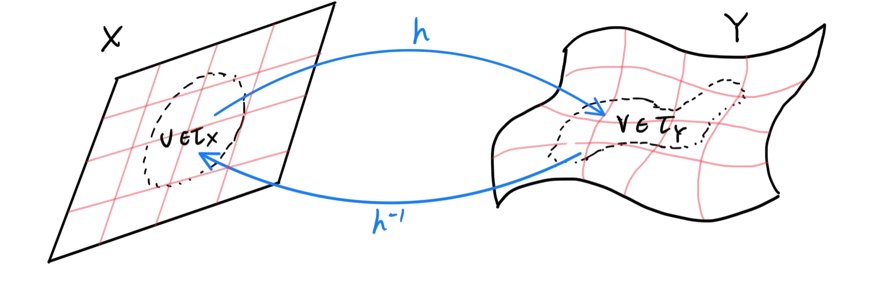
\includegraphics[scale=0.4]{img/Homeomorphism_of_Plane.png}
      \caption{The visual below shows a homeomorphism between the plane $X$ and the surface $Y$.}
      \label{fig:homeomorphism_plane}
    \end{figure}
  \end{definition}

  Note that it is easier for $f$ to be continuous when the $\T_X$ is finer (since there are more open sets in $X$ for the preimage of $V \subset Y$ to map to) or $\T_Y$ is coarser (since there are fewer open sets that we have to check to map to open sets of $X$). 

\subsection{Basis} 

  We want to continue analyzing the properties of a topology, but sometimes working with the entire topology is a bit thorny. There is a tamer representation of a topology, which can also give us the starting point to \textit{construct} topologies. 

  \begin{definition}[Basis] 
    \label{def:basis}
    If $X$ is a set, a \textbf{basis} on $X$ is a collection $\B$ of subsets of $X$ (called \textbf{basis elements}) such that
    \begin{enumerate}
      \item For each $x \in X$, there is at least one basis element $B \in \B$ containing $x$. That is, the elements of $\B$ covers $X$. 
      \item If $x$ belongs to the intersection of two basis elements $B_1$ and $B_2$, then there is a basis element $B_3$ containing $x$ such that $B_3 \subset (B_1 \cap B_2)$. 
    \end{enumerate}
  \end{definition} 

  The name gives away the clue that a topology may be created from this basis.  

  \begin{definition}[Basis to Topology]
    \label{def:basis-to-topology}
    Given a basis $\B$ on a set $X$, we can define a topology $\T$, called the \textbf{topology generated by $\B$}, in the following equivalent ways. 
    \begin{enumerate}
      \item $\T$ consists of subsets $U$ of $X$ satisfying the property that for each $x \in U$, there exists a basis element $B \in \B$ such that $x \in B \subset U$.\footnote{Note that since we can always set $U = \emptyset$, the basis doesn't need to contain $\emptyset$. }
      \begin{center}
        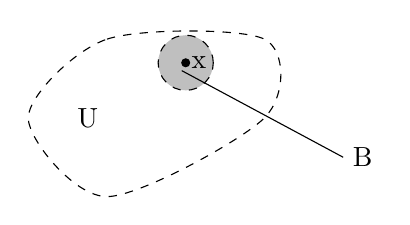
\begin{tikzpicture}
        \draw[dashed] plot [smooth cycle] coordinates {(0,0) (1,1) (3,1) (3,0) (1,-1)};
        \node [right] at (0.5,0) {U};
        \draw[fill=lightgray,dashed] (2,0.7) circle [radius=0.35];
        \draw[fill] (2, 0.7) circle [radius=0.05];
        \node [right] at (1.95,0.7) {x};
        \node [right] at (4,-0.5) {B};
        \draw (1.95,0.6)--(4,-0.5);
        \end{tikzpicture}
      \end{center}

      \item $\T$ consists of all possible unions of elements in $\B$. 
      \begin{equation}
        \T \coloneqq \Big\{ \bigcup_i B_i \mid B_i \in \B\Big\}
      \end{equation}
    \end{enumerate}
  \end{definition} 
  \begin{proof}
    We prove that the 2 methods generate a topology, and then finally prove that it they are the same topology. 
    \begin{enumerate}
      \item Clearly, $\emptyset$ and $X$ itself are in $\T$. To prove property 2, given a certain indexed family of subsets $\{U_\alpha\}_{\alpha \in I}$ of $\T$, we must show that 
      \begin{equation}
        U = \bigcup_{\alpha \in I} U_\alpha \in \T
      \end{equation}
      Given $x \in U$, there exists at least one index $\alpha$ such that $x \in U_\alpha$. Since $U_\alpha \in \T$ already, there exists a basis element $b \in \B$ such that $x \in b \subset U_\alpha$. But 
      \begin{equation}
        U_\alpha \subseteq U \implies b \subset U
      \end{equation}
      So, by definition, any arbitrary union of $U$ of these subsets is also in $\T$. 

      To prove property 3, we must show that 
      \begin{equation}
        W = \bigcap_{\alpha \in I} U_\alpha \in \T
      \end{equation}
      Given $x \in W$, by definition of a basis element, there exists a $b \in \B$ such that 
      \begin{equation}
        x \in b \subset (U_\beta \cap U_\gamma) \forall \beta, \gamma \in I \implies \text{ there exists } \Tilde{b} \in \B \text{ s.t. } x \in \Tilde{b} \subset \bigcap_{\alpha \in I} U_\alpha
      \end{equation}
      By definition, $W$ is also open. Since this arbitrary set of subsets $\T$ suffices the 3 properties, it is a topology of $X$ by definition. 

      \item $(\rightarrow)$ Given a collection of elements in $\B$, they are also elements of $\T$. Since $\T$ is a topology, their union in also in $\T$. 

      $(\leftarrow)$ Given an open set $U \in \T$, for every point $x \in U$, by definition we can choose a basis element $b \in \B$ such that $x \in b \subset U$. Then, the union of all these basis elements is by definition $b$. 
        
    \end{enumerate}
  \end{proof}

  We have learned how to go from a basis to a topology. The following lemma tells us how to identify a basis within a topology. 

  \begin{theorem}[Topology to Basis]
    Let $(X, \T)$ be a topological space, and let $\B$ be a collection of open subsets of $X$ such that for every open set $U$ and each $x \in U$, there exists an element $B \in \B$ such that
    \begin{equation}
      x \in B \subset U
    \end{equation}
    Then, $\B$ is a basis for the topology of $X$. 
  \end{theorem}
  \begin{proof}
    Note that there are two claims here: $\B$ is a basis and the topology that $\B$ generates is equal to $\T$. 
    \begin{enumerate}
      \item To prove that $\B$ is a basis, note that $X$ is an open set, and by assumption, for every $x \in X$, there exists a $B \in \B$ s.t. $x \in B \subset X$. Therefore $\B$ covers $X$. Now take two basis elements $B_1, B_2 \in \B$ with $x \in B_1 \cap B_2$. Since we know that $B_1, B_2$ are open, $B_1 \cap B_2$ is open and so for each $x \in B_1 \cap B_2$, there exists a basis element $B_3$ s.t. $x \in B_3 \in (B_1 \cap B_2)$. Thus $\B$ is a basis. 

      \item Let us call $\T^\prime$ the topology generated by $\B$. Then, given $U \in \T$, by assumption for any $x \in U$, there exists a basis element $B \in \B$ s.t. $x \in B \subset U$, so $x \in \T^\prime$. Conversely, if $U \in \T^\prime$, then $U$ is an arbitrary union of elements $B \in \B$ where each $B$ is open in $\T$, so $U \in \T$. So $\T = \T^\prime$. 
    \end{enumerate}
  \end{proof} 

  Characterizing topologies in terms of basis is quite effective since we can work with more manageable sets. 

  \begin{lemma}[Fineness w.r.t. Basis]
    Given two topologies $\T$ and $\T^\prime$ with their bases $\B$ and $\B^\prime$, respectively, the following are equivalent. 
    \begin{enumerate}
      \item $\T^\prime$ is finer than $\T$. 
      \item For each $x \in X$ and basis element $B \in \B$ containing $x$, there exists a basis element $B^\prime \in \B^\prime$ such that $x \in B^\prime \subset B$. 
    \end{enumerate}
  \end{lemma}

  So we have seen how we can take a collection of sets satisfying the basis properties and construct a topology as the union of the sets in this collection. What happens if we can relax some of these conditions? Note that the first condition was that the basis elements must cover $X$. This is non-negotiable. However, if we remove the second requirement that a basis element must be contained in an intersection of basis elements, we can get a \textit{subbasis}. 

  \begin{definition}[Subbasis]
    A \textbf{subbasis} $\mathscr{S}$ for a topology on $X$ is a collection of subsets of $X$ whose union is equal to $X$. 
  \end{definition}

  \begin{theorem}[Subbasis to Topology]
    Given a subbasis $\mathscr{S}$ on a set $X$, the \textbf{topology generated by $\mathscr{S}$} is defined to be the collection $\T$ of all unions of finite intersections of elements of $\mathscr{S}$. 
  \end{theorem}
  \begin{proof}
    It suffices to show that the collection of finite intersections of elements form a basis. 
  \end{proof}

  Now we show three extremely common topologies that can be constructed with bases. 

\subsection{Order Topology}

  \begin{definition}[Order Topology]
    \label{def:order-topology}
    Let $X$ be a set with a simple order relation. Let $\B$ be the collection of all sets of the following types.\footnote{If $X$ has no minimum or maximum, then there are no sets of type of 2 or 3, respectively.}
    \begin{enumerate}
      \item All open intervals $(a, b) \coloneqq \{x \in X \mid a < x < b\} \subset X$
      \item All half-open intervals $[a_0, b)$, where $a_0$ is the minimum element of $X$
      \item All half-open intervals $(a, b_0]$, where $b_0$ is the maximum element of $X$. 
    \end{enumerate}
    This set $\B$ is a basis for the \textbf{order topology} of $X$. 
  \end{definition}
  \begin{proof}
    We prove that this set $\mathscr{B}$ is a basis. 
    \begin{enumerate}
      \item It covers $X$. If $x \in X$ is the maximum or minimum we can cover it with $(a, b_0]$ and $[a_0, b)$, respectively. If not, then $x$ is bounded above and below, and so there exists $a, b \in X$ s.t. $a < x < b \implies x \in (a, b)$. 

      \item Let $x \in (a_1, b_1)$ and $x \in (a_2, b_2)$. Then, 
      \begin{equation}
        x \in (\max\{a_1, a_2\}, \min\{b_1, b_2\}) \in \mathscr{B} 
      \end{equation}
    \end{enumerate}
    Therefore, the generated collection is indeed a topology. 
  \end{proof}

  \begin{example}[Standard Order Topology on $\mathbb{R}$]
    The standard topology on $\mathbb{R}$ is precisely the order topology derived from the usual order on $\mathbb{R}$. Since $\mathbb{R}$ has no minimum or maximum, the basis consists of open intervals $(a, b) \subset \mathbb{R}$ with $a, b \in \mathbb{R}$. 
  \end{example}

  \begin{example}[Basis of Open Intervals with Rational Endpoints]
    We can however get away with smaller basis that generate the same topology on $\mathbb{R}$. If we take the set of all open intervals $(a, b) \subset \mathbb{R}$ with $a, b \in \mathbb{Q}$, this is also a basis for the same standard order topology. Too see why, let us denote this basis as $\B^\prime$ and the basis of all open intervals with real endpoints be $\B$. Then, clearly $B^\prime \subset \B \implies \T^\prime \subset \T$. As for the other, way, let us take an open interval $(a, b) \in \B$. Then we can see that 
    \begin{equation}
      (a, b) = \bigcup_{\substack{p, q \in \mathbb{Q} \\ a < p, q < b}} (p, q)
    \end{equation}
    where equality follows from density of rationals in $\mathbb{R}$. 
  \end{example}

  \begin{example}[$\mathbb{R}^2$ with Dictionary Order]
    Given $\mathbb{R} \times \mathbb{R}$ with the dictionary order, then $\mathbb{R} \times \mathbb{R}$ has neither a largest nor smallest element. Therefore, the order topology on $\mathbb{R} \times \mathbb{R}$ consists of all "intervals" of form
    \begin{equation}
      \big((a, b), (c, d) \big) \coloneqq  \{(x, y) \in \mathbb{R}^2 \mid (a, b) < (x, y) < (c, d)\}
    \end{equation}

    \begin{figure}[H]
      \centering 
      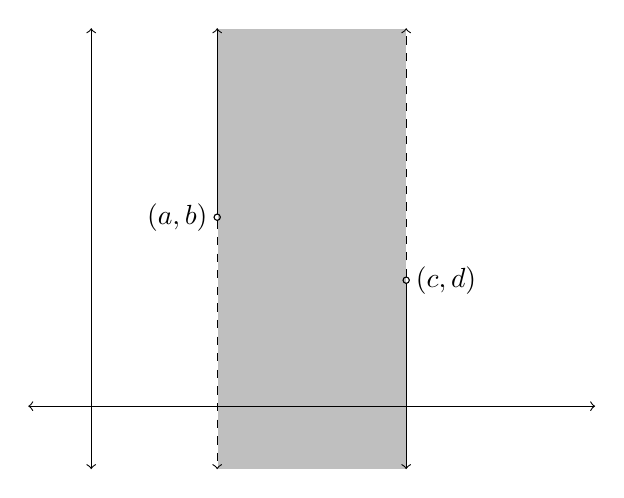
\begin{tikzpicture}[scale=0.8]
        \draw[white, fill=lightgray] (2,-1) rectangle (5,6);
        \draw[<->] (-1,0)--(8,0);
        \draw[<->] (0,-1)--(0,6);
        \draw[->] (2,3.05)--(2,6);
        \draw[->] (5,1.95)--(5,-1);
        \draw (2,3) circle [radius=0.05];
        \draw (5,2) circle [radius=0.05];
        \draw[dashed, ->] (2,2.95)--(2,-1);
        \draw[dashed,->] (5,2.05)--(5,6);
        \node[left] at (2,3) {$(a, b)$};
        \node[right] at (5,2) {$(c,d)$};
      \end{tikzpicture}
      \caption{This means that open rays and lines are also a part of the topology of $\mathbb{R} \times \mathbb{R}$. } 
      \label{fig:r2_dict_order}
    \end{figure}
  \end{example}

  \begin{example}[Positive Integers]
    The set of positive integers $\mathbb{Z}_+$ form an ordered set with a smallest element. The order topology for $\mathbb{Z}_+$ is precisely the discrete topology since every one-point set is an open set. 
    \begin{equation}
      \{n\} = (n-1, n+1)
    \end{equation}
  \end{example}

  \begin{example}[Two Copies of Positive Integers]
    The dictionary order topology on $\{1, 2\} \times \mathbb{Z}_+$ results in every one point set being open, except for the point $(2, 1)$. Since every neighborhood of $(2,1)$ must contain some point of form $(1, n)$ for arbitrarily large $n$, $\{(2,1)\}$ is not open. 
  \end{example}

  \begin{definition}
    If $X$ is an ordered set a $a \in X$, then there are 4 subsets of $X$ called rays determined by $a$. 
    \begin{enumerate}
      \item $(a, +\infty)$ 
      \item $(-\infty, a)$
      \item $[a, +\infty)$
      \item $(-\infty, a]$
    \end{enumerate}
    The first two sets are called \textbf{open rays}, and the latter two sets are called \textbf{closed rays}. 
  \end{definition}

  We can extend the basis of open intervals to some other basis based on the order, which generates other topologies. 

  \begin{example}[Lower/Upper Limit Topology]
    Given a totally ordered set $(X, \leq)$, 
    \begin{enumerate}
      \item the \textbf{lower limit topology} is the topology generated by the basis of all half-closed half-open intervals of form 
      \begin{equation}
        [a, b) \coloneqq \{ x \in X \mid a \leq x < b \}
      \end{equation}
      \item the \textbf{upper limit topology} is the topology generated by the basis of all half-open half-closed intervals of form 
      \begin{equation}
        (a, b] \coloneqq \{ x \in X \mid a < x \leq b \}
      \end{equation}
    \end{enumerate}
  \end{example}

  \begin{example}[Nested Interval Topology]
    In the space $X = (0,1)$, the \textbf{nested interval topology} is the topology generated by the basis of nested intervals of the form 
    \begin{equation}
      \B_{ni} \coloneqq \{ (0, 1-\frac{1}{n}) \mid n \in \mathbb{N} \}
    \end{equation}
  \end{example}

  A topology generated by closed intervals can also be a topology! 

  \begin{example}[Closed Interval Topology]
    In the set $X = [-1, 1]$, the following set 
    \begin{equation}
      \B_{ci} \coloneqq \{ [-1, a) \mid a > 0 \big\} \bigcup \big\{ (b, 1] \mid b<0 \}
    \end{equation}
    is a basis. The topology it generates is called the \textbf{closed interval topology}, denoted $\T_{ci}$. 
  \end{example}

  Finally, we talk about a seemingly arbitrary topology called the K-topology, but it is useful for counterexamples.   

  \begin{example}[K-Topology]
    In $\mathbb{R}$, let us denote $K = \{1/n\}_{n \in \mathbb{N}}$. Then the \textbf{K-topology} on $\mathbb{R}$ is the topology generated by the basis consisting of 
    \begin{enumerate}
      \item all open intervals $(a, b)$ with $a, b \in \mathbb{R}$. 
      \item all sets of the form $(a, b) \setminus K$ with $a, b \in \mathbb{R}$. 
    \end{enumerate}
  \end{example} 

  Now that we have some collection of topologies, let's try to compare them. We claim the following. 

  \begin{theorem}[Comparison of Topologies of the Real Line]
    
  \end{theorem}

\subsection{Metric Topology}

  For common sets like $\mathbb{R}^n$, which has an inner product, or $\mathbb{Q}$, which has an order, it is easy to build these topologies with set-builder notation. Consider the following. 

  \begin{definition}[Metric Topology]
    \label{def:metric-topology}
    Given a metric space $(X, d)$, let us denote the \textbf{metric topology}, or \textbf{open-ball topology}, as the set of subsets $U$ satisfying the property that for all $x \in U$, there exists a positive $r \in \mathbb{R}$ such that $B(x, r) \subset U$, where $B(x, r) \coloneqq \{y \in X \mid d(x, y) < r\}$ is the open ball of radius $r$ around $x$. We claim that this is a topology. 
  \end{definition} 
  \begin{proof}
    We show that the properties of a topology hold. 
    \begin{enumerate} 
      \item For the empty set, the inclusion of an open ball for a point in $\emptyset$ is vacuously satisfied. For the whole set, we choose any point $x$ and any $r$, and the open ball is trivially a subset of $X$. 

      \item Let $\{U_\alpha\}_{\alpha \in I}$ be a collection of open subsets of $X$. Let their union be denoted $U$. We claim $U$ is open. Pick any point $x \in U$. Then by definition of union, there exists some $\alpha \in I$ s.t. $x \in U_\alpha$. Since $U_\alpha$ is open, there exists a $r > 0$ s.t. $B(x, r) \subset U_\alpha \subset U$. Therefore $U$ is open. 

      \item Let $U_1, \ldots, U_k$ be open, and let us denote their intersection as $U$. We claim $U$ is open. Pick a point $x \in U$. Then for each $i = 1, \ldots, k$, $x \in U_i$ and there exists a corresponding $r_i > 0$  such that the open ball $B(x, r_i) \subset U_i$. Take the set $R = \{r_i\}$, which is a finite set living in $\mathbb{R}$. We will take for granted that every finite subset of an ordered set has a minimum.\footnote{If we wish to prove it, we can start with a singleton set, claim that its minimum is the only element. Then we use induction by assuming for a set $R$ of size $k$ that a minimum exists, and by adding $1$ more element $r$ we update the minimum to be $\min\{r, \min{R}\}$ and show that this is indeed the minimum.} Let us denote $r^\ast = \min{R}$, and we claim that $r^\ast$ gives us a ball that can fit inside $U$. Assume $y \in B(x, r^\ast)$. Then 
      \begin{align}
        y \in B(x, r^\ast) & \implies d(x, y) < r^\ast \\ 
                           & \implies d(x, y) < \min{R} \\
                           & \implies d(x, y) < r_i \text{ for } i = 1, \ldots, k \\
                           & \implies y \in B(x, r_i) \text{ for } i = 1, \ldots, k
      \end{align} 
      Since $B(x, r_i)$ by construction is contained within $U_i$, $y \in U_i$ for all $i$. This means by definition of intersection that $y \in U$, and we have proven that $B(x, r^\ast)$ completely fits inside $U$. 
    \end{enumerate}
  \end{proof} 

  Note that while open balls are used to define whether a set is open or not, the definition doesn't state whether open balls themselves are open sets. It turns out that it is easy to prove that they are. 
  
  \begin{lemma}[Open Balls are Open Sets]
    The open ball wrt any metric $d$ is an open set wrt the metric topology. 
  \end{lemma}
  \begin{proof}
    Let $y \in B(x, r)$. Then $d(x, y) < r \implies 0 < r - d(x, y)$. To show that $B(x, r)$ is open, we would like to show that there exists some $r^\prime > 0$ s.t. $y \in B(y, r^\prime) \subset B(x, r)$. Set $r^\prime = r - d(x, y)$. Then 
    \begin{align}
      z \in B(y, r^\prime) & \implies d(y, z) < r - d(x, y) \\
                           & \implies d(x, y) + d(x, y) < r \\
                           & \implies d(x, z) < r \\
                           & \implies z \in B(x, r)
    \end{align} 
    and so $B(y, r^\prime) \subset B(x, r)$. We are done. 
  \end{proof}

  \begin{example}[Discrete Metric Induces Discrete Topology]
    Given a set $X$, induce the metric $d$ defined
    \begin{equation}
      d(x, y) \coloneqq \begin{cases} 1 & \text{if } x \neq y \\ 0 & \text{if } x = y \end{cases}
    \end{equation}
    This metric induces the discrete topology on $X$, since the basis elements of the open balls
    \begin{equation}
      B_r (x) \coloneqq \{ y \in X \mid d(x, y) <r\}
    \end{equation}
    consists of two types of open sets. When $r \leq 1$, then $B_r (x) = x$ (since the radius is $0$). If $r > 1$, then the open set is the entire space $X$. 
  \end{example} 

  While the behavior for finite sets are predictable under the metric topology, as soon we we get into infinite sets, the properties of the metric topology may differ. 

  \begin{example}[Metric Topologies on $\mathbb{Z}$ and $\mathbb{Q}$]
    $\mathbb{Z}$ and $\mathbb{Q}$ are countable sets, so there is a bijection between them. If we give each of them the metric topology, $\mathbb{Z}$ ends up having the discrete topology (take the $0.5$-ball around each integer), whereas for $\mathbb{Q}$, we will see later that by the density of the rationals there are an infinite number of rationals in $(q - r, q + r)$ for $q \in \mathbb{Q}$. Therefore, the metric topology may or may not induce the discrete topology. 
  \end{example}

  \begin{example}[Supremum Norm in $\mathbb{R}^3$]
    \begin{figure}[H]
      \centering 
      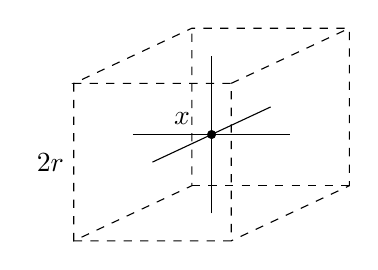
\begin{tikzpicture}
        \draw[dashed] (0,0)--(2,0)--(2,2)--(0,2)--(1.5,2.7)--(3.5,2.7)--(3.5,0.7)--(2,0);
        \draw[dashed] (2,2)--(3.5,2.7);
        \draw[dashed] (0,2)--(0,0)--(1.5,0.7)--(1.5,2.7);
        \draw[dashed] (1.5,0.7)--(3.5,0.7);
        \draw (1,1)--(2.5,1.7);
        \draw (0.75,1.35)--(2.75,1.35);
        \draw (1.75,0.35)--(1.75,2.35);
        \draw[fill] (1.75,1.35) circle (0.05);
        \node[above left] at (1.6,1.35) {$x$};
        \node[left] at (0,1) {$2r$};
      \end{tikzpicture}
      \caption{In $\mathbb{R}^3$, each basis element is a cube centered at $x$ with side lengths $2r$.} 
      \label{fig:sup_norm_R3}
    \end{figure}
  \end{example}

  \begin{theorem}[Metric Topologies on Finite Sets]
    If $(X, d)$ is a finite metric space, then the metric topology on it is the discrete topology. 
  \end{theorem}
  \begin{proof}
    Take all pairwise points and compute $\epsilon = \min_{x \neq y} \{d(x, y)\}$. Since $X$ is finite, all pairs are finite and therefore the minimum exists. Now let us take the $\epsilon$-ball around $x$. Then every $y \neq x$ has distance $d(x, y) \geq \epsilon$, and therefore $y \not\in B(x, \epsilon)$. So all single points are open sets, which induces the discrete topology. 
  \end{proof}

  A finite set $S$ of points does not have any limit points, since if we draw small enough circles around a $p \in S$, then at some point the circle will not contain any more points (remember that we're talking about deleted neighborhoods). Following this, we can deduce that a limit point must always have an infinite number of points close to it, as in no matter how small the circle gets, there are always an infinite number of points contained within that circle. This also means that if $p$ is a limit point, then we can construct a sequence of points in $S$ that converges to $p$, since every open ball with smaller and smaller radii will still have points in $S$.

  \begin{theorem}[Neighborhood of Limit Point Contains Infinite Points in Metric Space]
    Let $X$ be a metric space. If $p$ is a limit point of $S$, then every neighborhood of $p$ contains infinitely many points of $S$. The converse is also true trivially. 
  \end{theorem}
  \begin{proof}
    Assume $p$ is a limit point and that there exists a finite number of points within a deleted neighborhood $B_r^\circ (p)$. Then, we can enumerate them $p_1, p_2, \ldots, p_n$ by their distances to $p$, with 
    \begin{equation}
      d(p_1, p) \leq d(p_2, p) \leq \ldots \leq d(p_n, p)
    \end{equation}
    Since $p_1 \neq p$, we have $d(p_1, p) > 0$ and so, we can choose an $0 < \epsilon < d(p_1, p)$ s.t. $B_\epsilon^\circ (p)$ does not contain any of the $p_i$'s. This neighborhood does not contain any elements of $S$ and so $p$ is not a limit point. 
  \end{proof}

  \begin{corollary}[Finite Set in Metric Space has No Limit Points]
    Let $X$ be a metric space and $S = \{s_i\}_{i=1}^n$ be a finite set. Then, $S^\prime = \emptyset$.  
  \end{corollary}
  \begin{proof}
    If $S$ is a finite set, then every neighborhood of every point $p$ in $\mathbb{R}^n$ will have at most finite points, which, by the previous theorem, is not a limit point. 
  \end{proof}

  \begin{lemma}[Fineness of Metric Topologies]
    Let $d$ and $d^\prime$ be two metrics on the set $X$ with their respective induced topologies $\T, \T^\prime$. We claim that $\T \subset \T^\prime$ iff there exists a $M > 0$ s.t. 
    \begin{equation}
      d^\prime (x, y) < M \cdot d(x, y)
    \end{equation} 
    for all $x, y \in X$. That is, we can bound $d^\prime$ with a constant multiple of $d$. 
  \end{lemma}
  \begin{proof}
    
  \end{proof}

  More specifically, the metric topology generated by the $L_2$-metric on $\mathbb{R}^n$ is called the \textbf{Euclidean topology}. Note that the topological property of stability under countable intersection was required to show that the minimum of $R$ existed. This is not true for infinite sets in general. This gives us some motivation as to why we need the \textit{finite} intersection rather than an infinite one. 
  
  \begin{lemma}[Singletons are Not Open in $\mathbb{R}^n$]
    A singleton set is not open in $\mathbb{R}^n$ with the Euclidean topology.   
  \end{lemma}
  \begin{proof}
    We claim that the singleton set $S = \{0\}$ is not open under the Euclidean metric. We pick a point in $S$, which can only be $0$. Assume that there exists an $r > 0$ s.t. $B(x, r) \subset S$. $\mathbb{R}$ is Archimedean, so there exists a natural number $N$ s.t. $0 < 1/N < r$. We construct the vector $v = (v_1, \ldots, v_n)$ s.t. $v_1 = 1/N$ and $v_i = 0$ everywhere else. The distance between $0$ and $v$ is 
    \begin{equation}
      \| v - 0 \| = \|v\| = \sqrt{(1/N)^2} = 1/N < r
    \end{equation} 
    so $v \in B(x, r)$. But $v \neq 0$, and by contradiction such an $r$ cannot exist. In $\mathbb{R}^n$ we consider the countable intersection of open balls (which we have proved in class are open sets) around $0$ of radius $1/N$ for $n \in \mathbb{N}$. We claim that 
    \begin{equation}
      \bigcap_{n \in \mathbb{N}} B(0, 1/n) = \{0\}
    \end{equation} 
    We see that $1/n$ must always be positive and so $\|0 - 0\| = 0 < 1/n$. Therefore the LHS $\supset $ RHS. To see that the intersection contains no other element, consider any vector $v \neq 0$. Then by definition of the metric, $d(v, 0) > 0$. By the Archimedean property, there exists a natural $N \in \mathbb{N}$ s.t. $0 < 1/N < d(v, 0)$, which means that $v \not\in B(0, 1/N)$, and so $v$ cannot be in the intersection. Therefore, the intersection must be $\{0\}$, and we have shown that $B_0$ is not open, so we are done. 
  \end{proof}

  \begin{theorem}[Metric Topology is Always Finer than Cofinite]
    For a metric space $(X, d)$, the metric topology is finer than the cofinite topology. 
  \end{theorem} 
  \begin{proof}
    Note that if $X$ is finite, then both are reduced to the discrete topologies. 
  \end{proof}

  While it is not surprising that a basis uniquely generates a topology, it is not immediately obvious \textit{what} the generated topology looks like. It turns out that many different bases may generate the same topology, and the concept of fineness allows us to compare these topologies more effectively. For example, if two topologies are both finer than the other, then they must be equal. 

  \begin{theorem}[Euclidean Topology on $\mathbb{R}^n$]
    \label{thm:lp-norms-euclidean-topology}
    $L^p$ norms all generate the same topology on $\mathbb{R}^n$. 
  \end{theorem}
  \begin{proof}
    We can show that 
    \begin{equation}
      n^q d_\infty \leq n^q d_2 \leq n^q d_1 \leq d_p \leq n^{-p} d_\infty
    \end{equation}
    where $q$ is the holder conjugate of $p$. Visually, we can see that every open ball in $(\mathbb{R}^n, d)$ (with the Euclidean metric) is the form to the left, while an open ball in $(\mathbb{R}^n, \rho)$ (with the square metric) is of form on the right. 
    \begin{center}
      \begin{tikzpicture}[scale=0.5]
        \draw [dashed] (1,0) circle [radius=2];
        \draw [dashed] (6,-2) rectangle (10,2);
        \draw [fill] (1,0) circle [radius=0.05];
        \node [above left] at (1,0) {x};
        \draw (1,0)--(3,0);
        \node [above] at (1.5,0) {r};
        \draw [fill] (8,0) circle [radius=0.05];
        \node [below right] at (8,0) {x};
        \draw (8,0)--(10,0);
        \draw (8,0)--(8,2);
        \node [right] at (8,1) {r};
        \node [above] at (9,0) {r};
      \end{tikzpicture}
    \end{center}
    Clearly, we can form any open set of any "shape" using any arbitrary combination of these "circles" or "squares," indicating that they generate the same topology. 
  \end{proof}

  \begin{theorem}[Convergence of Sequence in Metric Space]
    Let $(X, d)$ be a metric space. $x$ is the limit of $(x_n)$ if it satisfies one of the two equivalent conditions: 
    \begin{enumerate}
      \item if $x_n \to x$ under the metric topology generated by $d$
      \item $\forall \epsilon > 0$, $\exists N \in \mathbb{N}$ such that
      \begin{equation}
        n \geq N \implies d(x_n, x) < \epsilon 
      \end{equation}
    \end{enumerate}
  \end{theorem}

  \begin{theorem}[Limit of a Function between Metric Spaces][def:limfunc-met]
    Let $f: E \subset X \to Y$ be a map between metric spaces and $p \in X$ be a limit point of $E$. We say $f(x) \to q$ as $x \to p$, i.e. 
    \begin{equation}
      \lim_{x \to p} f(x) = q
    \end{equation} 
    if it meets the following equivalent conditions. 
    \begin{enumerate}
      \item \textit{$\epsilon$-$\delta$ Definition}. If $\forall \epsilon > 0$, $\exists \delta > 0$ s.t. $0 < d_X (x, p) < \delta \implies d_Y (f(x), q)) < \epsilon$.

      \begin{figure}[H]
        \centering 
        \begin{tikzpicture}
          \node at (0, 3) {$X$};
          \node at (6.5, 3) {$Y$};
          
          % Function arrow
          \draw[->, thick, bend left=20] (2.5,1.5) to node[above] {$f$} (6.5,1.5);
          
          % Blue blob 1 - made bigger but still in top left
          \draw[blue, thick, dashed] plot [smooth cycle, tension=0.8] coordinates {(0.2,1.7) (0.6,1.2) (1.0,0.9) (1.5,1.0) (1.8,1.4) (1.6,1.9) (1.3,2.3) (0.9,2.5) (0.5,2.4) (0.2,2.2)};
          \fill[blue, pattern=north west lines, pattern color=blue, opacity=0.2] plot [smooth cycle, tension=0.8] coordinates {(0.2,1.7) (0.6,1.2) (1.0,0.9) (1.5,1.0) (1.8,1.4) (1.6,1.9) (1.3,2.3) (0.9,2.5) (0.5,2.4) (0.2,2.2)};
          \node at (1.0,0.4) [blue] {$f^{-1}(B_\epsilon(q))$};
          
          % Blue blob 2 - in bottom right
          \draw[blue, thick, dashed] plot [smooth cycle, tension=0.7] coordinates {(1.8,0.8) (2.2,0.6) (2.6,0.7) (2.8,1.0) (2.7,1.3) (2.3,1.2) (2.0,1.1)};
          \fill[blue, pattern=north west lines, pattern color=blue, opacity=0.2] plot [smooth cycle, tension=0.7] coordinates {(1.8,0.8) (2.2,0.6) (2.6,0.7) (2.8,1.0) (2.7,1.3) (2.3,1.2) (2.0,1.1)};
          
          % Left neighborhood (red, hatched circle) - moved inside V1
          \draw[red, thick, dashed] (1.2,1.6) circle (0.4);
          \fill[red, pattern=north east lines, pattern color=red, opacity=0.3] (1.2,1.6) circle (0.4);
          \node at (2.2,2) [red] {$\mathring{B}_\delta(p)$};
          
          % Point p - hollow and red - also moved
          \draw (1.2,1.6) circle (0.05);
          \node at (1.2,1.6) [below right] {$p$};
          
          % Right neighborhood (blue circle)
          \draw[blue, thick, dashed] (8,1.5) circle (1);
          \fill[blue, pattern=north west lines, pattern color=blue, opacity=0.2] (8,1.5) circle (1);
          \node at (8.5,2.6) [blue] {$B_\epsilon(q)$};
          
          % Point q - where f(p) would be, now just a point reference
          \draw (8,1.5) circle (0.05);
          \node at (8,1.5) [below right] {$q$};
          
          % Epsilon visualization - dotted line segment not touching the blue boundary
          \draw[blue, thick, dotted] (8,1.5) -- (9,1.5) node[midway, above] {$\varepsilon$};
        \end{tikzpicture}
        \caption{Said in one line, the preimage of any open ball around $y = f(x)$ must contain some open deleted open ball around $x$.} 
        \label{fig:limit_function}
      \end{figure}

      \item \textit{Sequential Definition}. If for all sequences $(x_n) \to p$, $f(x_n) \to q$.

      \begin{figure}[H]
        \centering 
        \begin{tikzpicture}[scale=1]
          % Space labels without axes
          \node at (1, 3) {$X$};
          \node at (7.5, 3) {$Y$};
          
          % Function arrow
          \draw[->, thick, bend left=20] (3.5,1.5) to node[above] {$f$} (7.5,1.5);
          
          % Point a in domain - shifted by 1
          \fill (2.5,1.5) circle (0.07);
          \node at (2.5,1.5) [above right] {$p$};
          
          % Blue sequence (x_n) in domain - curved path - shifted by 1
          \filldraw[blue] (1.3,0.6) circle (0.03);
          \filldraw[blue] (1.7,0.8) circle (0.03);
          \filldraw[blue] (1.9,1.0) circle (0.03);
          \filldraw[blue] (2.1,1.3) circle (0.03);
          \filldraw[blue] (2.3,1.4) circle (0.03);
          \node at (1.6,0.4) [blue] {$(x_n)$};
          
          % Red sequence (y_n) in domain - curved path - shifted by 1
          \filldraw[red] (2.7,1.6) circle (0.03);
          \filldraw[red] (2.9,1.7) circle (0.03);
          \filldraw[red] (3.0,1.8) circle (0.03);
          \filldraw[red] (3.2,1.85) circle (0.03);
          \filldraw[red] (3.5,1.9) circle (0.03);
          \node at (3.4,2.0) [red] {$(y_n)$};
          
          % Point A in codomain
          \fill (8,1.5) circle (0.07);
          \node at (8,1.5) [above right] {$q$};
          
          % Blue sequence (f(x_n)) in codomain - curved path
          \filldraw[blue] (7.1,0.7) circle (0.03);
          \filldraw[blue] (7.3,0.9) circle (0.03);
          \filldraw[blue] (7.5,1.1) circle (0.03);
          \filldraw[blue] (7.7,1.2) circle (0.03);
          \filldraw[blue] (7.8,1.4) circle (0.03);
          \node at (7.2,0.4) [blue] {$(f(x_n))$};
          
          % Red sequence (f(y_n)) in codomain - curved path
          \filldraw[red] (8.2,1.7) circle (0.03);
          \filldraw[red] (8.5,1.8) circle (0.03);
          \filldraw[red] (8.7,2.0) circle (0.03);
          \filldraw[red] (8.9,2.3) circle (0.03);
          \filldraw[red] (9.1,2.5) circle (0.03);
          \node at (9.2,1.9) [red] {$(f(y_n))$};
        \end{tikzpicture}
        \caption{For every sequence that converges to the left, the new sequence mapped through $f$ converges to $q$. Note that we choose the points $x_n$ to be in the "deleted" neighborhood $E\setminus a$ (neighborhood $E$ with point $a$ removed) to force us to choose a sequence that is not $a, a, \ldots$. That is, it forces us to choose different points for the sequence. } 
        \label{fig:sequential_limit_def}
      \end{figure}
    \end{enumerate}
  \end{theorem}
  \begin{proof}
    We prove equivalence. 
    \begin{enumerate}
      \item $(\to)$. Assume $\lim_{x \to p} f(x) = q$. Let $(x_n) \in E$ s.t. $x_n \to p$ with $x_n \neq p$. We wish to show that $f(x_n) \to q$. Let $\epsilon > 0$. Then $\exists \delta > 0$ s.t. $0 < d_X (x, p) < \delta \implies d_Y (f(x), q) < \epsilon$. Since $\delta > 0$, by definition $\exists N \in \mathbb{N}$ s.t. if $n \geq N$, $d_X (x_n , p) < \delta \implies d_Y (f(x_n), q)$. 
    \end{enumerate}
  \end{proof}

  Sometimes, the $\epsilon$-$\delta$ definition is good, but a lot of the times the sequential definition is good enough and more insightful. Note also that the topological definition of a limit does not include the sequential definition because it is not true.\footnote{\href{https://math.stackexchange.com/a/3151525/616717}{https://math.stackexchange.com/a/3151525/616717}}

  \begin{example}[Counterexample]
    
  \end{example}

  \begin{theorem}[Analytic Continuity = Topological Continuity] 
    Given metric spaces with their induced metric topologies $(X, \T_X, d_X)$ and $(Y, \T_Y, d_Y)$. The following are equivalent. 
    \begin{enumerate}
      \item $f: X \rightarrow Y$ is continuous at $x$. 
      \item For every $\delta > 0$, there exists an $\epsilon = \epsilon(\delta) > 0$ such that for all $z \in X$, $d_X (x, z) < \epsilon \implies d_Y (f(x), f(x)) < \delta$.\footnote{This is the definition of continuity at a point in analysis.} 
    \end{enumerate}
  \end{theorem}
  \begin{proof}
    ($\rightarrow$) Assume $f$ is continuous according to the $\epsilon - \delta$ definition. Let $U$ be any open set in $Y$ containing the point $y$, and let $x$ be an element in $f^{-1}(U)$ such that $y = f(x)$. We must prove that $f^{-1}(U)$ is also open. Since open sets contain neighborhoods (e.g. open balls) of all of its points, we can claim that, since $U$ is open by assumption, there exists an open ball $B_y$ around $y$ with radius $\epsilon > 0$. This guarantees the existence of a point $z \in U$ such that $\rho(y, z) < \epsilon$ for any $\epsilon > 0$ that we choose. Since $f$ is continuous, for every $\epsilon >0$ that we chose previously, there exists a $\delta >0$ such that $d(x, w) \implies \rho(f(x), f(w)) < \epsilon$. Since $\rho(f(x), f(w)) < \epsilon$, we can conclude that $f(w) \in B_y \subset U$ when $d(x, w) < \delta$. Therefore, $d(x, w) < \delta \implies w \in f^{-1}(U)$. But this is equivalent to saying that if $w \in B_(x, \delta)$, then $w \in f^{-1}(U)$, which means that every single point $x \in f^{-1}(U)$ contains an open ball neighborhood fully contained in $f^{-1}(U)$. So, by definition, $f^{-1}(U)$ is open. 


    ($\leftarrow$) Assume $f^{-1}(U)$ is open when $U$ is an open set in $Y$, i.e. $f$ is continuous under the topological definition. Let us define the open ball 
    \begin{equation}
      B(f(x), \epsilon) \coloneqq \{ y \in Y \mid \rho(f(x), y) < \epsilon\} \in \mathscr{T}_Y
    \end{equation}
    By our assumption, $f^{-1} \big( B(f(x), \epsilon) \big)$ is an open set in $\mathscr{T}_X$, and clearly, $x \in f^{-1} \big( B(f(x), \epsilon) \big)$ since $f^{-1}$ maps the point $f(x) \in B(f(x), \epsilon)$ to $x \in f^{-1} \big( B(f(x), \epsilon) \big)$. But since $f^{-1} \big( B(f(x), \epsilon) \big)$ is open, we can construct an open ball around $x$ with radius $\delta$ fully contained within the open set. Moreover, by selecting a point $p \in B(f(x), \delta) \subset f^{-1}\big( B(f(x), \epsilon) \big)$, we can guarantee that $f(p) \in B(f(x), \epsilon)$. This is precisely the $\epsilon - \delta$ definition of continuity. That is, given an $\epsilon > 0$ to be the radius of an open ball $B(f(x), \epsilon)$ in $Y$, we can always choose a $\delta > 0$ to be the radius of the open ball $B(x, \delta)$ in $X$ that is fully contained within the preimage of $B(f(x), \epsilon)$. In mathematical notation, 
    \begin{equation}
      p \in B(x, \delta) \subset f^{-1} \big( B(f(x), \epsilon) \big) \implies f(p) \in f\big( B(x, \delta) \big) \subset B(f(x), \epsilon)
    \end{equation}
    or equivalently in terms of metrics,
    \begin{equation}
      d(x, p) < \delta \implies \rho (f(x), f(p)) < \epsilon
    \end{equation}
  \end{proof} 

\subsection{Initial and Final Topologies} 

  We have seen some examples of how to create topologies. They can be created without any assumptions on the set, such as the discrete, indiscrete, and the cofinite topologies. More often, we want to consider how a certain structure like the order or a metric induces a topology. Now, we will consider how \textit{functions} can induce a topology. The uniqueness of such induced topologies is called the \textit{universal property}. 

  \begin{definition}[Initial Topology]
    Given a space $X$ and a family of topological spaces $\{Y_\alpha\}_{\alpha \in A}$ 
    \begin{equation}
      f_i : X \rightarrow (Y_\alpha, \T_\alpha)
    \end{equation} 
    the \textbf{initial topology} on $X$ is the coarsest topology $\T$ on $X$ s.t. that each 
    \begin{equation}
      f_i (X, \T) \rightarrow (Y_\alpha, \T_\alpha)
    \end{equation}
    is continuous. 
  \end{definition}

  \begin{definition}[Final Topology]
    Given a space $Y$ and a family of topological spaces $\{X_\alpha\}_{\alpha \in A}$ 
    \begin{equation}
      f: (X, \T_\alpha) \rightarrow Y
    \end{equation}
    the \textbf{final topology} on $Y$ is the finest topology $\T$ on $Y$ s.t. each 
    \begin{equation}
      f: (X, \T_\alpha) \rightarrow (Y, \T)
    \end{equation}
    is continuous. 
  \end{definition}

  Note that it makes sense to talk about the coarsest topology on the domain and the finest topology on the codomain. If it were the other way around, i.e. the finest topology on the domain, then the initial topology on $X$ would be the discrete topology, making every function defined on $X$ continuous. In the same logic, the coarsest topology on $Y$ would trivially be the trivial topology, making all $Y$-valued functions continuous. With these current definitions, if $\T_Y$ is too fine (e.g. if $\T_Y = 2^Y$), then the open sets of $\T_Y$ would be too fine and therefore would have a preimage that may not be open in $X$. 

\subsection{Subspace Topology} 

  The reason we want to do this is because we want to think of $Y$ as its own entity, independent of $X$. 

  \begin{definition}[Subspace Topology]
    Given topological space $X$ and subspace $Y \subset X$, the \textbf{subspace topology} on $Y$ is defined in the equivalent ways. 
    \begin{enumerate}
      \item It is the initial topology on the subspace $Y$ with respect to the inclusion map $\iota: Y \rightarrow X$. 
      \item It is the topology consisting of $X$-open sets intersection $Y$.
      \begin{equation}
        \T_Y = \{(U \cap Y) \subset Y \mid U \in \T_X\}
      \end{equation}
      We can also say that $A \subset Y$ is closed in $Y$ iff it is the inersection of $Y$ with a closed set of $X$. 
    \end{enumerate}

    \begin{figure}[H]
      \centering
      \begin{subfigure}[b]{0.48\textwidth}
        \centering
        \begin{tikzpicture}
          % Draw the x and y axes in gray
          \draw[gray] (-3,0) -- (3,0);
          \draw[gray] (-1,-2) -- (-1,2);
          
          % Draw a blob (open set) with dotted borders
          \draw[dotted, thick] plot [smooth cycle, tension=0.8] coordinates {(-1,1) (0,1.5) (1.5,1) (2,-0.5) (1,-1.5) (-0.5,-0.8) (-1.5,-0.2)};
          
          % Label the open set
          \node at (0.0,0.8) {$U \in \mathscr{T}_{\mathbb{R}^2}$};
          
          % Draw a straight line passing through the blob with arrows on both ends
          \draw[-{Stealth[length=3mm]}, blue] (-2.5,-1.8) -- (2.5,1.8);
          
          % Label the line
          \node[anchor=north, blue] at (1.5,2) {$\ell \subset \mathbb{R}^2$};
          
          % Bold the portion where the line intersects the blob
          % Calculate or estimate intersection points
          \draw[thick, red] (-0.9,-0.65) -- (1.4, 1.0);
          
          % Label the intersection
          \node[red, anchor=south west] at (0,-0.7) {$V \in \mathscr{T}_\ell$};
          
          % Draw circles at the intersection points
          \draw[red] (-0.9,-0.65) circle (0.05);
          \draw[red] (1.4,1.0) circle (0.05);
        \end{tikzpicture}
        \caption{The subspace topology of a line $l$ in $\mathbb{R}^2$.}
        \label{fig:subspacer2}
      \end{subfigure}
      \hfill 
      \begin{subfigure}[b]{0.48\textwidth}
        \centering
        \tikzset{
          pattern size/.store in=\mcSize, 
          pattern size = 5pt,
          pattern thickness/.store in=\mcThickness, 
          pattern thickness = 0.3pt,
          pattern radius/.store in=\mcRadius, 
          pattern radius = 1pt}
          \makeatletter
          \pgfutil@ifundefined{pgf@pattern@name@_kou00hae2}{
          \pgfdeclarepatternformonly[\mcThickness,\mcSize]{_kou00hae2}
          {\pgfqpoint{0pt}{0pt}}
          {\pgfpoint{\mcSize+\mcThickness}{\mcSize+\mcThickness}}
          {\pgfpoint{\mcSize}{\mcSize}}
          {
          \pgfsetcolor{\tikz@pattern@color}
          \pgfsetlinewidth{\mcThickness}
          \pgfpathmoveto{\pgfqpoint{0pt}{0pt}}
          \pgfpathlineto{\pgfpoint{\mcSize+\mcThickness}{\mcSize+\mcThickness}}
          \pgfusepath{stroke}
        }}
        \makeatother
        \tikzset{every picture/.style={line width=0.75pt}}        
        \begin{tikzpicture}[x=0.75pt,y=0.75pt,yscale=-0.7,xscale=0.7]
          \draw  [color=blue,draw opacity=1][dash pattern={on 4.5pt off 4.5pt}] (291.17,116.36) .. controls (291.17,108.7) and (311.31,102.5) .. (336.17,102.5) .. controls (361.02,102.5) and (381.17,108.7) .. (381.17,116.36) .. controls (381.17,124.01) and (361.02,130.21) .. (336.17,130.21) .. controls (311.31,130.21) and (291.17,124.01) .. (291.17,116.36) -- cycle ;
          \draw    (272.32,35.59) .. controls (324.17,100.5) and (372.92,78.58) .. (470.17,20.5) ;
          \draw    (182.17,197.5) .. controls (273.66,272.15) and (386.17,172.5) .. (446.17,203.5) ;
          \draw    (272.32,35.59) .. controls (245.26,184.08) and (242.74,206.43) .. (182.17,197.5) ;
          \draw    (470.17,20.5) .. controls (501.17,119.5) and (470.17,190.5) .. (446.17,203.5) ;
          \draw  [color=blue,draw opacity=1][dash pattern={on 4.5pt off 4.5pt}] (285.17,138.12) .. controls (285.22,109.89) and (308.14,87.05) .. (336.37,87.1) .. controls (364.6,87.15) and (387.45,110.07) .. (387.4,138.3) .. controls (387.35,166.53) and (364.42,189.37) .. (336.19,189.33) .. controls (307.96,189.28) and (285.12,166.35) .. (285.17,138.12) -- cycle ;
          \draw  [color=red,draw opacity=1][pattern=_kou00hae2,pattern size=6pt,pattern thickness=0.75pt,pattern radius=0pt, pattern color=red][dash pattern={on 4.5pt off 4.5pt}] (337.41,141.34) .. controls (358.41,126.34) and (400.91,124.76) .. (380.91,144.76) .. controls (360.91,164.76) and (310.91,174.76) .. (290.91,144.76) .. controls (270.91,114.76) and (316.41,156.34) .. (337.41,141.34) -- cycle ;
          \draw  [color=blue,draw opacity=1][dash pattern={on 4.5pt off 4.5pt}] (302.17,173.86) .. controls (302.17,168.69) and (317.39,164.5) .. (336.17,164.5) .. controls (354.94,164.5) and (370.17,168.69) .. (370.17,173.86) .. controls (370.17,179.02) and (354.94,183.21) .. (336.17,183.21) .. controls (317.39,183.21) and (302.17,179.02) .. (302.17,173.86) -- cycle ;

          \node at (225,100) {$S \subset \mathbb{R}^3$};
          \node[blue] at (430,138) {$U \in \mathscr{T}_{\mathbb{R}^3}$};
          \node[red] at (240,150) {$V \in \mathscr{T}_{S}$};
        \end{tikzpicture}
        \caption{The subspace topology of a surface $\mathcal{L}$ in $\mathbb{R}^3$.}
        \label{fig:subspacer3}
      \end{subfigure}
      \caption{Visual of subspace topology.}
      \label{fig:subspace_topology}
    \end{figure}
  \end{definition} 
  \begin{proof}
    We prove the properties. 
    \begin{enumerate}
      \item \textit{Trivial}. We see that $\emptyset = \emptyset \cap Y$ and $Y = X \cap Y$. 
      \item \textit{Stability under Union}. Suppose $\{V_\alpha\}_{\alpha \in A}$ are setes that are open in $Y$. Then for each $\alpha$ there exists an open set $U_\alpha \subset X$ that is open in $X$. Therefore, 
      \begin{align}
        \bigcup_{\alpha \in A} V_\alpha & = \bigcup_{\alpha \in A} (U_\alpha \cap Y) \\ 
                                        & = Y \cap \bigg( \bigcup_{\alpha \in A} U_\alpha \bigg)
      \end{align}
      where $\cup_\alpha U_\alpha$ is open in $X$, and therefore we shown that there exists such an open set. 

      \item \textit{Stability under Finite Intersection}. Suppose $\{V_i\}_{i = 1}^n$ are open in $Y$. Then we can do the same thing. 
    \end{enumerate}
  \end{proof} 

  Furthermore, we can immediately retrieve the basis of the subspace topology. 

  \begin{theorem}[Induced Basis of Subspace Topologies]
    If $\B$ is a basis for the topology of $X$, then 
    \begin{equation}
      \B_Y \coloneqq \{B \cap Y \mid B \in \B \} 
    \end{equation}
    is a basis for the subspace topology of $Y$. 
  \end{theorem}
  \begin{proof}
    
  \end{proof} 

  Now if the subspace $Y$ were to be an open or closed subset of $X$, the properties of openness and closedness carry over nicely. 

  \begin{lemma}[Open/Closed Subspaces]
    Let $X$ be a topological space, $Y \subset X$ have the subspace topology, and $S \subset Y$. 
    \begin{enumerate}
      \item If $Y$ is open in $X$, then $S$ open in $Y$ iff $S$ open in $X$. 
      \item If $Y$ is closed in $X$, then $S$ closed in $Y$ iff $S$ closed in $X$. 
    \end{enumerate}
  \end{lemma}

  Since the subspace is so natural to consider, we will by default imply that if $X$ is a topological space and $Z \subset X$, $Z$ is endowed the subspace topology. 

  \begin{lemma}[Restrictions and Injections are Continuous]
    The results immediately follow: 
    \begin{enumerate}
      \item Given $f: X \rightarrow Y$ and $Z \subset X$, $f|_{Z} : Z \rightarrow Y$ is continuous. 
      \item Given $X$ and $Z \subset X$, the canonical injection $\iota: Z \rightarrow X$ is continuous. 
    \end{enumerate}
  \end{lemma}

  Consider any set $U \subset Y$. Note that if $U$ is an open set in $X$ that happens to be contained in $Y$, then we can set $U = U \cap Y$, so $U$ is open in $Y$. However, we have seen that being open in $Y$ does not necessarily imply that it is open in $X$. 

  \begin{example}[Non-Open Sets may be Open in Subspace]
    Let $X = \mathbb{R}$ with the Euclidean topology and let $Y = [0, 1]$. 
    \begin{enumerate}
      \item $[0, 1]$ is open in $Y$ but not open in $X$. 
      \item Intervals of the form $(a, 1]$ and $[0, b)$ are open in $Y$ but not open (nor closed) in $X$. 
    \end{enumerate}
  \end{example} 

  \begin{example}[Singleton Sets in Subspace Topologies]
    Consider $X = \mathbb{R}$ with the lower limit topology with $Y = [0, 1]$. The following 
    \begin{enumerate}
      \item $[1/2, 1] = Y \cap [1/2, 2)$, and 
      \item $\{1\} = Y \cap [1, 2)$
    \end{enumerate}
    are open in the subspace topology. It turns out that $\{1\}$ is the only singleton set open in $Y$. 
  \end{example}

  Let's go through a few examples. 

  \begin{example}[Closed Unit Interval in $\mathbb{R}$]
    The basis for the subspace topology of $[0, 1] \subset \mathbb{R}$ with the Euclidean topology consists of the intervals 
    \begin{enumerate}
      \item $(a, b)$ where $0 \leq a < b \leq 1$. 
      \item $[0, b)$ where $0 < b \leq 1$. 
      \item $(a, 1]$ where $0 \leq a < 1$. 
    \end{enumerate}
  \end{example} 

  \begin{example}[Unit Sphere in $\mathbb{R}^n$] 
    Let $S^n \subset \mathbb{R}^{n+1}$ be the unit \textbf{n-sphere} defined $S^n \coloneqq \{x \in \mathbb{R}^{n+1} \mid ||x||^2 = 1 \}$. When thinking about $S^n$ as a space itself, we use the subspace topology coming from the standard topology of $\mathbb{R}^n$. 
  \end{example}

  \begin{example}[$S^1 \subset \mathbb{R}^2$]
    Let's focus on $n = 1$. For $a < b$, let 
    \begin{equation}
      A_{a, b} = \{ (\cos{t}, \sin{t}) \mid a < t < b \}
    \end{equation} 
    Then, we can see that
    \begin{enumerate}
      \item if $b - a > 2 \pi$, then $A_{a, b} = S^1$. 
      \item If $b - a \leq 2 \pi$, then $A_{a, b}$ is an ``open arc'' from $(\cos{a}, \sin{a})$ to $(\cos{b}, \sin{b})$.  
    \end{enumerate} 

    Given that we have an equivalence class defined 
    \begin{equation}
      A_{a, b} \sim A_{a + 2 \pi k, b + 2 \pi k} \text{ for all } k \in \mathbb{Z}
    \end{equation} 
    We claim that $\{A_{a, b}\}$ is a basis for the subspace topology of $S^1$. We can see that the open arc covering the top right quadrant in $\mathbb{R}^2$ is 
    \begin{equation}
      S^1 \cap (0, 1)^2 = S^1 \cap B_\infty \big( (\frac{1}{2}, \frac{1}{2}), \frac{1}{2} \big)
    \end{equation}
  \end{example}

  Now let's focus more on metric spaces. Note that if we want to construct topologies of subspaces of metric spaces, there are two ways to do it. It would be quite bad if these resulted in different topologies, but fortunately we have the following theorem. 

  \begin{theorem}[Topologies on Subspaces of Metric Spaces Coincide]
    Let $(X, d_X)$ be a metric space, with $Y \subset X$. There are 2 ways we can define a topology on $Y$. 
    \begin{enumerate}
      \item Take the metric topology $\T_X$ on $X$, and then take the subspace topology on $Y$. 
      \item Induce a metric $d_Y = d_{X | Y}$ on $Y$ which is a restriction of $d_X$ to $Y$, and then take the metric topology of it. 
    \end{enumerate}
    We claim that these two constructions give the same topology, as shown in the commutative diagram. 

    \begin{figure}[H]
      \centering 
      \begin{tikzcd}
        d_X \arrow[r] \arrow[d] & d_Y \arrow[d] \\
        \T_X \arrow[r] & \T_Y 
      \end{tikzcd}
      \caption{} 
      \label{fig:same_construction}
    \end{figure}
  \end{theorem}
  \begin{proof}
    The basis for the subspace topology on $Y$ is 
    \begin{equation}
      \B_1 = \{B_{d_X} (x, r) \cap Y \mid x \in X, r > 0 \}
    \end{equation} 
    and the basis for the (induced) metric topology on $Y$ is 
    \begin{equation}
      \B_2 = \{B_{d_Y} (y, r) \cap Y \mid y \in Y, r > 0 \} = \{B_{d_X} (y, r) \cap Y \mid y \in Y, r > 0 \}
    \end{equation} 
    It is immediate that $\B_2 \subset \B_1$ since it goes over all $x \in X$ rather than $y \in Y$. To see why $\B_1 \subset \B_2$, TBD. 
  \end{proof}

  \begin{theorem}[Closures in Subspace Topologies]
    Let $A \subset Y \subset X$. Let $\bar{A}$ denote the closure of $A$ in $X$. Then, the closure of $A$ in $Y$ equals $\bar{A} \cap Y$. 
  \end{theorem}

\subsection{Box and Product Topologies} 

  There are multiple ways to define the box and product topologies, but their construction with basis elements is most simple. 

  \begin{definition}[Box Topology]
    Given a family of topological spaces $\{(X_\alpha, \T_\alpha)\}_{\alpha \in A}$, the \textbf{box topology} on the space $\prod_{\alpha \in A} X_\alpha$ is the topology generated by the basis 
    \begin{equation}
      \mathscr{B} = \bigg\{ \prod_{\alpha \in A} U_\alpha \mid U_\alpha \in \T_\alpha \bigg\}
    \end{equation}

    \begin{figure}[H]
      \centering 
      \begin{tikzpicture}
        \draw[<->] (-1,0)--(6,0);
        \draw[<->] (0,-1)--(0,4);
        \draw[dashed] (1,1)--(1,3)--(4,3)--(4,1)--(1,1);
        \node[below] at (6,0) {$\mathbb{R}$};
        \node[left] at (0,4) {$\mathbb{R}$};
        \node[below] at (1,-0.3) {$a$};
        \node[below] at (4,-0.3) {$b$};
        \node[left] at (-0.3,1) {$c$};
        \node[left] at (-0.3,3) {$d$};
        \node[rotate=90] at (0,1) {$($};
        \node[rotate=-90] at (0,3) {$($};
        \node at (1,0) {$($};
        \node at (4,0) {$)$};
      \end{tikzpicture}
      \caption{We can visualize the elements of the box topology with the product space $\mathbb{R}^2 = \mathbb{R} \times \mathbb{R}$, where each $\mathbb{R}$ has an open ball topology. From the visual below, we can see why this is called the "box" topology. }
      \label{fig:box_topology}
    \end{figure}
  \end{definition}
  \begin{proof}
    It is easy to prove that the box topology indeed satisfies the 3 properties of topologies in general. 
  \end{proof}
	
  While the box topology may seem quite "intuitive" for the first learner, the box topology however, has serious limitations when extending to infinite Cartesian products of spaces. To motivate the product topology, let's try to ``reverse engineer'' a topology on $X \times Y$ such that the projection mappings $\pi_1: X \times Y \rightarrow X$ is always continuous. We want 
  \begin{enumerate}
    \item $U \times Y$ to be open for $U \subset X$ open. 
    \item $X \times V$ to be open for $V \subset Y$ open. 
  \end{enumerate}
  This implies that $(U \times Y) \cap (X \times V) = U \times V$ should be open. This is how we will define the product topology. The main difference between the construction of open sets in the box topology vs the product topology is that the box topology merely describes open sets as direct products of open sets from each coordinate space while the construction of the product topology is completely dependent on the projection mappings $\pi_\beta: \prod_{\alpha \in I} X_\alpha \rightarrow X_\beta$ to be continuous (and nothing more) so that (by definition) the preimages of open sets in $X_\beta$ under $\pi_\beta$ are open sets in $\prod X_\alpha$. Therefore, the construction of the continuous $\pi_\beta$'s canonically constructs a basis of open sets in $\prod X_\alpha$. 

  \begin{definition}[Product Topology] 
    \label{def:product-topology}
    Given a family of topological spaces $\{(X_\alpha, \T_\alpha)\}_{\alpha \in A}$, the \textbf{product topology} on the space $\prod_{\alpha \in A} X_\alpha$ is defined in the following equivalent ways. 
    \begin{enumerate}
      \item It is the initial topology on the product space wrt the family of projections $p_\alpha: \prod_{\alpha \in A} X_\alpha \rightarrow X_\alpha$. 

      \item It is the topology generated by the basis of elements 
      \begin{equation}
        \prod_\alpha U_\alpha 
      \end{equation}
      where $U_\alpha$ is a proper open subset for at most finitely many $\alpha$'s, and $U_\alpha = X_\alpha$ for all other $\alpha$. 
    \end{enumerate}

    \begin{figure}[H]
      \centering 
      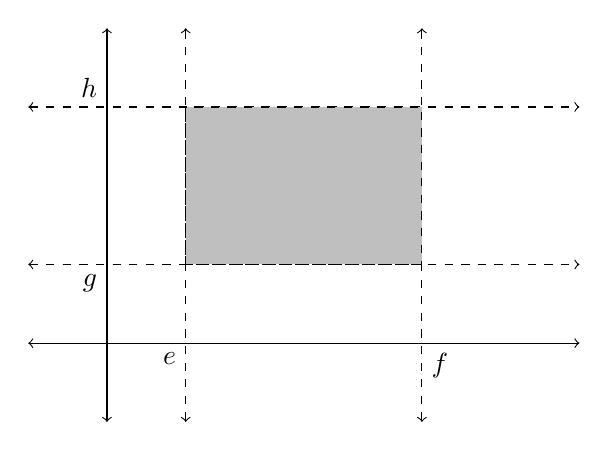
\begin{tikzpicture}
        \draw[<->] (-1,0)--(6,0);
        \draw[<->] (0,-1)--(0,4);
        \draw[<->, dashed] (-1,1)--(6,1);
        \draw[<->, dashed] (-1,3)--(6,3);
        \draw[<->, dashed] (1,-1)--(1,4);
        \draw[<->, dashed] (4,-1)--(4,4);
        \node [below left] at (1,0) {$e$};
        \node [below right] at (4,0) {$f$};
        \node [above left] at (0,3) {$h$};
        \node [below left] at (0,1) {$g$};
        \draw[dashed, fill=lightgray] (1,1) rectangle (4,3);
      \end{tikzpicture}
      \caption{Visually, we can interpret each $\mathscr{S} (U_\beta)$ as a "strip" in the total product space. For example in $\mathbb{R}^2$, there are two "strips" $(e, f) \times \mathbb{R}$ and $\mathbb{R} \times (g, h)$ that intersect. Note that each strip is the preimage of the projection mapping. }
      \label{fig:product_topology}
    \end{figure}
  \end{definition}

  We can deduce some conclusions comparing these topologies. First, the product and box topologies are precisely the same if we work in finite Cartesian products of spaces, since any element of the box topology (left hand side) can be expressed as a finite intersection of some open sets (in the right hand side). That is, if $\text{card}\,I < \infty$, then 
  \begin{equation}
    \prod_{\alpha \in I} U_i = \bigcap_{\alpha \in I} \big\{ \prod_{\gamma \in I} W_\gamma \mid W_\gamma = U_\gamma \text{ if } \gamma = \alpha, \, W_\gamma = X_\gamma \text{ if } \gamma \neq \alpha\big\}
  \end{equation}
  Secondly, we can see that the box topology is finer than the product topology (strictly finer if working in infinite product spaces). 

  \begin{example}
    The set $(0,1)^\mathbb{N} \subset \mathbb{R}^\mathbb{N}$ is clearly open in the box topology, but it is considered "too tight" to be in the product topology. However, 
    \begin{equation}
      (0,1) \times \mathbb{R} \times \mathbb{R} \times \ldots
    \end{equation}
    is open in the product topology since only one (a finite amount) of the factors is not the whole space. 
  \end{example}

  The following theorem reveals why the product topology is superior than the box topology in product spaces. 

  \begin{theorem}[Continuity of Functions Mapped to Product Topology]
    Given the function 
    \begin{equation}
      f: A \rightarrow \prod_{\alpha \in I} X_\alpha, \; f(a) \coloneqq \big( f_\alpha (a) \big)_{\alpha \in I}
    \end{equation}
    with its component functions $f_\alpha: A \rightarrow X_\alpha$. Let $\prod X_\alpha$ have the product topology. Then the function $f$ is continuous if and only if each function $f_\alpha$ is continuous. 
  \end{theorem}
  \begin{proof}
    We prove both directions. Let $\pi_\beta$ be the projection of this product onto the $\beta$th component space. By construction $\pi_\beta$ is continuous $\implies \pi_\beta^{-1} (U_\beta)$ is a basis element of the product topology of $\prod X_\alpha$. 
    \begin{enumerate}
      \item $(\rightarrow)$ $f$ is continuous, so $f_\beta \coloneqq \pi_\beta \circ f$, as the composition of continuous functions, is also continuous. 
      \item $(\leftarrow)$ Assume that each $f_\beta$ is continuous. Let there be an open set $U_\beta \subset X_\beta$. Then, the canonical open set $\pi_\beta^{-1}$ in the product space $\prod X_\alpha$ is also open. Now, the preimage of $\pi_\beta^{-1} (U_\beta)$ under $f$ is 
      \begin{align*}
        f^{-1} \big( \pi_\beta^{-1} (U_\beta)\big) & = (f^{-1} \circ \pi_\beta^{-1})(U_\beta) \\
        & = (\pi_\beta \circ f)^{-1} (U_\beta) \\
        & = f_\beta^{-1} (U_\beta)
      \end{align*}
      Since $f_\beta$ is already assumed to be continuous, $f_\beta^{-1} (U_\beta)$ is open in $A$. 
    \end{enumerate}
  \end{proof} 

  This theorem also works for the box topology only if we are working with finite product spaces. But in general, this theorem fails for the box topology. Consider the following example. 

  \begin{example}
    Let $\mathbb{R}^\omega$ be the countably infinite product of $\mathbb{R}$'s. Let us define the function 
    \begin{equation}
      f: \mathbb{R} \rightarrow \mathbb{R}^\omega
    \end{equation}
    with coordinate function defined $f_n (t) \coloneqq t$ for all $n \in \mathbb{N}$. Clearly, each $f_n$ is continuous. Given the box topology, we consider one basis element of $\mathbb{R}^\omega$
    \begin{equation}
      B = \prod_{i=1}^\infty (-\frac{1}{i}, \frac{1}{i})
    \end{equation}
    Assume that $f$ is continuous, that is $f^{-1}(B)$ is open in $\mathbb{R}$. Then, it would contain some finite interval $(-\delta, \delta)$ about $0$, meaning that $f\big( (-\delta, \delta)\big) \subset B$. This implies that for each $n \in \mathbb{N}$, 
    \begin{equation}
      f_n \big( (-\delta, \delta) \big) = (-\delta, \delta) \subset \Big( -\frac{1}{n}, \frac{1}{n} \Big)
    \end{equation}
    which contradicts the fact that $B$ is open, since the interval $(-1/n, 1/n)$ converges onto a point $0$. 
  \end{example}

  However, there is no useful criterion for the continuity of a mapping $f: X \times Y \longrightarrow A$ even if we have the product topology on $X \times Y$. One might conjecture that this $f$ is continuous if it is continuous in each variable separately, but this is in fact not true. 

  \begin{theorem}[Topologies on Products of Metric Spaces Coincide]
    Given a metric space
  \end{theorem}

  \begin{corollary}
    The Euclidean topology on $\mathbb{R}^n$ is equivalent to the product topology of the Euclidean topologies on $\mathbb{R}$. 
  \end{corollary} 

  \begin{theorem}[Subspace of Products and Products of Subspaces are Equivalent]
    If $A \subset X$ and $B \subset Y$, then the following topologies are equivalent. 
    \begin{enumerate}
      \item The subspace topology on the product topology of $X \times Y$. 
      \item The product topology on the subspace topologies of $A, B$. 
    \end{enumerate}
  \end{theorem}

  \begin{example}[Sorgenfrey Plane]
    The Cartesian product of two real lines with the lower limit topology is called the \textbf{Sorgenfrey plane}. 
    \begin{equation}
      \mathbb{R}_\ell \times \mathbb{R}_\ell
    \end{equation}
  \end{example}

  \begin{lemma}
    The addition, subtraction, and multiplication operations are continuous functions from $\mathbb{R} \times \mathbb{R} \longrightarrow \mathbb{R}$, and the quotient operation is a continuous function from $\mathbb{R} \times (\mathbb{R} \setminus \{0\}) \longrightarrow \mathbb{R}$. 
  \end{lemma}
  \begin{proof}
    Standard $\epsilon-\delta$ proof. 
  \end{proof}

  Now that we have defined what it means for binary operations to be continuous, we can talk about \textit{topological algebra}, which is the study of algebraic structures such that their algebraic operations and inverses are continuous. One important such concept is a \textit{topological group}, which will be mentioned later. 

\subsection{Quotient Topologies} 

  We have established natural topologies on sets that are constructed from other sets, namely by subsets and Cartesian products. Another way to construct a set is by taking an equivalence relation, which partitions the set into its equivalence classes. Then, we would like to construct a natural topology on this new set of equivalence classes. Such a topology is called a quotient topology. Note that we can completely describe an equivalence class $\sim$ on $X$ with a surjective function $p: X \to X/\sim$ such that 
	\begin{equation}
	  x \sim x^\prime \iff p(x) = p(x^\prime)
	\end{equation}

	Given an element $[x] \in X/\sim$, the elements that are in the equivalence class $[x]$ is $p^{-1}([x])$. This set is known as \textit{saturated}. 

  \begin{definition}[Saturated Sets]
    A subset $A \subset X$ is \textbf{saturated} with respect to the surjective map $p: X \rightarrow Y$ if it satisfies the equivalent definitions. 
		\begin{enumerate}
			\item $p^{-1} \big( p(A) \big) = A$. 
			\item There exists a set $B \subset Y$ s.t. $A = p^{-1}(B)$. 
			\item If $a \in A$ and $x \in X$ satisfy $p(x) = p(a)$, then $x \in A$. 
		\end{enumerate}

    \begin{figure}[H]
      \centering 
      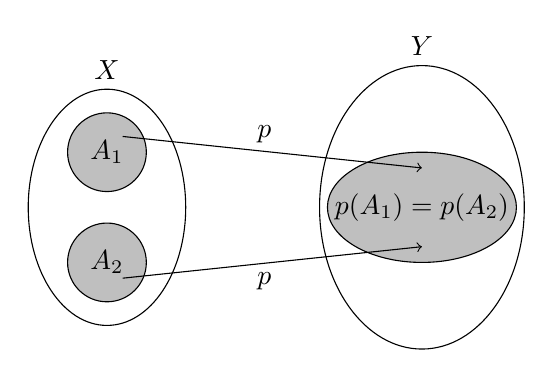
\begin{tikzpicture}
        \draw (0,0) ellipse (1 and 1.5);
        \draw[fill=lightgray] (0, 0.7) circle (0.5);
        \draw[fill=lightgray] (0, -0.7) circle (0.5);
        \node[above] at (0,1.5) {$X$};
        \draw (4,0) ellipse (1.3 and 1.8);
        \node[above] at (4,1.8) {$Y$};
        \draw[fill=lightgray] (4,0) ellipse (1.2 and 0.7);
        \node at (0, 0.7) {$A_1$};
        \node at (0,-0.7) {$A_2$};
        \node at (4,0) {$p(A_1) = p(A_2)$};
        \draw[->] (0.2,0.9)--(4,0.5);
        \draw[->] (0.2,-0.9)--(4,-0.5);
        \node[above] at (2, 0.7) {$p$};
        \node[below] at (2, -0.7) {$p$};
      \end{tikzpicture}
      \caption{We can see that $A_1$ and $A_2$ alone are not saturated, but $A_1 \cup A_2$ is saturated. Visually, for a given set $A \subset X$ to be saturated, there cannot be any points $q \not\in A$ such that $q \in p(A)$. }
      \label{fig:saturation}
    \end{figure}
  \end{definition}
	\begin{proof}
	  We prove equivalence. 
		\begin{enumerate}
		  \item $(1) \rightarrow (2)$. Set $B = p(A)$. 
			\item $(2) \rightarrow (3)$. Let $a \in A, x \in X$ with $p(x) = p(a)$. By hypothesis, there exists a set $B \subset Y$ s.t. $A = p^{-1}(B) \implies B = p(A)$. So, $p(a) \in B \implies p(x) \in B$. Therefore, $x \in p^{-1}(p(x)) \subset A$. 
			\item $(3) \rightarrow (1)$. Let $B = p(A)$. Then, $p^{-1} (p(A)) \supset A$.  Let $x \in p^{-1} (p(A)) \subset X$. Then, there exists an $a \in A$ s.t. $x = p^{-1}(p(a)) \implies p(x) = p(a)$. By hypothesis, this implies that $x \in A$. Therefore, $p^{-1}(p(A)) \subset A \implies p^{-1}(p(A)) = A$. 
		\end{enumerate}
	\end{proof}

	We have characterized sets that look like potential equivalence classes. Now, we generalize the surjective function $p$ that defines such equivalence classes. 

  \begin{definition}[Quotient Map]
    A function $p: X \rightarrow Y$ is said to be a \textbf{quotient map} if it satisfies the equivalent definitions. 
		\begin{enumerate}
		  \item $p$ is surjective and for every $U \subset Y$, 
				\begin{equation}
					U \text{ is open/closed in } Y \iff p^{-1}(U) \text{ is open/closed in } X
				\end{equation} 

			\item $p$ is continuous, surjective, and if $A \subset X$ is open (closed) and saturated, then $p(A) \subset Y$ is open (closed). 
		\end{enumerate}
  \end{definition}
	\begin{proof}
	  We prove bidirectionally. 
		\begin{enumerate}
			\item $(\rightarrow)$. $p$ is surjective and continuous by the right implication. Now if $A \subset X$ is open and saturated, then there exists a $B \subset Y$ s.t. $p^{-1}(B) = A$. Therefore $p^{-1}(B)$ is open in $X$, and from (1), $B = p(A)$ must be open in $Y$. 
			\item $(\leftarrow)$. $p$ is surjective and continous, which proves the right implication. Now let $B \subset Y$ be some subset such that $A = p^{-1} (B)$ is open in $X$. Then, $A$ is saturated because $p^{-1}(p(A)) = p^{-1}(p(p^{-1}(B))) = p^{-1}(B) = A$, and so by (2), $p(A) = B$ is open. 
		\end{enumerate}
	\end{proof}

	\begin{example}[Quotient Map that Sticks Two Intervals Together]
    Let $X \coloneqq [0,1] \cap [2,3] \subset \mathbb{R}$ and $Y \coloneqq [0,2] \subset \mathbb{R}$. Then, we define $p: X \rightarrow Y$ as 
    \begin{equation}
      p(x) \coloneqq \begin{cases} x & x \in [0,1] \\ x-1 & x \in [2,3] \end{cases}
    \end{equation}
    $p$ is continuous (under subspace topology of $X \subset \mathbb{R}$), surjective, and closed, meaning that it is a quotient map. However, it is not open, since the image of the open set $[0,1]$ of $X$ is $[0,1]$, which is not open in $Y$. 
  \end{example}

  The first property is that quotient maps behave nicely under compositions. 

  \begin{lemma}[Composition of Quotient Maps]
    The composition of two quotient maps is a quotient map. 
  \end{lemma}
  \begin{proof}
    We immediately know that the composition of surjective maps are surjective and that of continuous maps are continuous. 
  \end{proof}

  However, they do not behave nicely under subspace or products. If $p: X \rightarrow Y$ is a quotient map and $A$ is a subspace of $X$, then the map $p^\prime: A \rightarrow p(A)$ obtained by restricting both the domain and codomain of $P$ need not be a quotient map. The product of two quotient maps is not necessarily a quotient map. That is, given $p: A \rightarrow B$ and $q: C \rightarrow D$ are quotient maps, the map 
  \begin{equation}
    p \times q: A \times C \rightarrow B \times D, \; (p \times q) (a \times c) \coloneqq p(a) \times q(c)
  \end{equation}
  is not necessarily a quotient map. 

  \begin{example}[Restriction of Quotient Maps are Not Quotient Maps]
    
  \end{example}

  \begin{example}[Products of Quotient Maps are Not Quotient Maps]
    
  \end{example}

  Additionally, quotient maps are clearly not homeomorphisms, so topological properties are not preserved. However, there is just one extra condition on a quotient map that will make it a homeomorphism.  

  \begin{lemma}[Bijective Quotient Maps]
    A quotient map that is injective (and hence bijective) is a homeomorphism. 
  \end{lemma} 

	\begin{lemma}
    Let $p: X \to Y$ be a continuous map. If there is a continuous map $f: Y \to X$ s.t. $p \circ f$ is the identity map, then $p$ is a quotient map. 
  \end{lemma}
  \begin{proof}
    Let $U \subset Y$ and let $p^{-1} (U)$ be open. Then, 
    \begin{align}
      p^{-1} (U) \text{ open } & \implies f^{-1} (p^{-1} (U)) \subset Y \text{ open} \\ 
                               & \implies (p \circ f)^{-1}(U) = U \subset Y \text{ open}
    \end{align}
    and since $p$ is continuous, $p$ is a quotient map. Since $p \circ f$ is the identity, it must follow that $p$ is surjective. 
  \end{proof}

  Now that we have defined the quotient map, we are ready to define the quotient topology. The intuition is the following. The topology on $X$ is fixed, and we must somehow find some topology on $Y$ that makes $p$ a quotient map. If we make $\T_Y$ too coarse, satisfiying continuity of $p$ is easy but it may not necessarily mean that $p^{-1}(U)$ open in $X$ implies $U$ open in $Y$. However, if we make $\T_Y$ too fine, then continuity may not be satisifed. The theorem states that there is a middle point---in fact exactly one topology---in which cases both directions are satisfied. 

  \begin{definition}[Quotient Topology]
    Let $p: (X, \T_X) \rightarrow Y$ be a surjective map.\footnote{A natural surjective map that we can construct is by taking an equivalence relation $\sim$ on $X$, setting $Y = X/{\sim}$, and taking $p: x \mapsto [x]$. Every surjective map can be thought of as a map induced by an equivalence relation, since we can set $x \sim x^\prime$ iff $f(x) = f(x^\prime)$, so these are equivalent.} Then, the \textbf{quotient topology} induced by $p$ is defined in the following equivalent ways. 
    \begin{enumerate}
      \item It is the final topology on the quotient set $X/{\sim}$ wrt the projection map $p$. 
      \item It is the topology of all subsets $U$ of $Y$ s.t. $p^{-1}$ is open in $X$. 
      \begin{equation}
        U \text{ open in } X/{\sim} \iff p^{-1} (U) \text{ saturated and open in } X
      \end{equation}
      \item It is the unique topology $\T_Y$ relative to which $p$ is a quotient map.\footnote{We claim that this topology exists and is unique.}
    \end{enumerate}
    The quotient set $X/{\sim}$ with its quotient topology is called the \textbf{quotient space}. 
  \end{definition}
  \begin{proof}
    The topology $\T_Y$ on $Y$ is defined by letting it consist of all subsets $U$ of $Y$ such that $p^{-1}(U)$ is open in $X$. This is indeed a topology since
    \begin{enumerate}
      \item $p^{-1} (\emptyset) = \emptyset$ and $p^{-1}(Y) = X$
      \item $p^{-1} \Big( \bigcup_{\alpha \in J} U_\alpha \Big) = \bigcup_{\alpha \in J} p^{-1} (U_\alpha)$
      \item $p^{-1} \Big( \bigcap_{i=1}^n U_i \Big) = \bigcap_{i=1}^n p^{-1} (U_i)$
    \end{enumerate}
  \end{proof}

  \begin{example}[Quotient Topology of a Finite Space]
    Let $p: \mathbb{R} \rightarrow \{a, b, c\}$ be defined as 
    \begin{equation}
      p(x) \coloneqq \begin{cases} a & x > 0 \\ b & x < 0 \\ c & x = 0 \end{cases}
    \end{equation}
    Then, the quotient topology of $\{a, b, c\}$ consists of 
    \begin{equation}
      \emptyset, \{a\}, \{b\}, \{a, b\}, \{a, b, c\}
    \end{equation}
  \end{example}

  \begin{example}[Quotient Topology Reduced to Trivial Topology]
    \label{quotient_trivial}
    Let $X = \mathbb{R}$ with $x \sim y \iff x - y \in \mathbb{Q}$. We claim that $X/{\sim}$ is uncountable. If we wish to find open sets in $X/{\sim}$, we can do this by finding saturated open sets in $X$. Let $U \subset \mathbb{R}$ be open and saturated. Since it is open, by the density of $\mathbb{Q}$ in $\mathbb{R}$, $U$ must contain a rational number $\implies \mathbb{Q} \subset U$, and so $U = \mathbb{R}$. Therefore the only saturated open sets are $\emptyset, \mathbb{R}$, meaning that $X/{\sim}$ has the trivial topology. 
  \end{example}

  Okay, so we've learned yet another way to construct topologies. However, things become interesting when we start to compare quotient spaces to other topological spaces that we already know of. The following series of theorems will help in our analysis. 

	\begin{theorem}[Universal Property of the Quotient Spaces]
		\label{thm:universal_quotient}
		\label{thm:quotient_homeomorphism}
    Let $p: X \rightarrow X/\sim$ be a quotient map. Let $f: X \rightarrow Y$ be a function such that if $p(x) = p(x^\prime)$, then $f(x) = f(x^\prime)$, i.e. $x \sim x^\prime \implies f(x) = f(x^\prime)$. Then, 
    \begin{enumerate}
			\item There exists a unique map $\Tilde{f}$ satisfying $f = \Tilde{f} \circ p$. 

      \begin{figure}[H]
        \centering 
        \begin{tikzcd}
          X \arrow{d}{p} \arrow{r}{f} & Y\\
					X/{\sim} \arrow[dashed]{ru}{\Tilde{f}} & 
        \end{tikzcd}
        \caption{The theorem states that the diagram commutes. } 
        \label{fig:quotient_continuity}
      \end{figure}

      \item $f$ continuous iff $\Tilde{f}$ continuous. 
      \item $f$ quotient map iff $\Tilde{f}$ quotient map. 
    \end{enumerate}

		Furthermore, we have $x \sim x^\prime \iff f(x) = f^\prime(x)$, then the induced map 
		\begin{equation}
			\Tilde{f}: X/\sim \to Y, \quad \Tilde{f}([x]) = [f(x)] 
		\end{equation}
		is a homeomorphism. 
  \end{theorem}
  \begin{proof}
    Listed. 
    \begin{enumerate}
      \item 
      \item Suppose $f$ is continuous. Let $U \subset Z$ be open. Then we need to show that $\bar{f}^{-1} (U)$ is open. But we can see that $p^{-1} (\bar{f}^{-1}(U)) = f^{-1} (U)$ is open since $f$ is continuious. Therefore $\bar{f}^{-1} (U)$ is open since $p$ is a QM.If $\bar{f}$ is continuous, then $f = \bar{f} \circ p$ is continuous as the composition of continuous maps. 
      \item Suppose $f$ is a quotient map with $U \subset Z$ s.t. $\bar{f}^{-1} (U)$ is open. We need to show that $U$ is open. Then $p^{-1} (\bar{f}^{-1} (U))$ is open since $p$ is continuous $\implies f^{-1} (U)$ is open. But $f$ is a quotient map, so $U$ is open. 
    \end{enumerate}
    For the final claim, how that $\Tilde{f}$ is injective, and so its bijective. Since it's a quotient map, it's a homeomorphism. 
  \end{proof}

  Therefore we can just make up any equivalence relation (surjective map) on $X$ which gives us a quotient space $X/{\sim}$. To figure out whether this quotient space is homeomorphic to a topological space that we already know, we first (cleverly) choose a candidate space $Z$ and try to write a quotient map $f: X \rightarrow Z$ that ``agrees'' with the equivalence relation, i.e. $x \sim x^\prime \iff f(x) = f(x^\prime)$. We don't need to worry too much about surjectivity, since if we have continuity and the ``reverse continuity'' conditions satisfied then we can just restrict $Z$ to the image of $f$ to make it surjective anyways. Once we have found such a quotient map $f$, using the theorem above we can conclude that $X/{\sim}$ is homeomorphic to $Z$, and we are done! We show various examples in the next section. 

	\begin{definition}[Wedge Sum]
		Given spaces $X, Y$ with chosen points $x_0 \in X, y_0 \in Y$, we define the \textbf{wedge sum} as
		\begin{equation}
			X \vee Y \coloneqq \frac{X \sqcup Y}{\sim}, \quad x_0 \sim y_0
		\end{equation}
	\end{definition}

	\begin{definition}[Cell]
		Let $X$ be a topological space. An \textbf{$n$-cell} is a subspace $e^n \subset X$ homeomorphic to the closed unit ball
		\begin{equation}
			\mathring{D}^n = \{x \in \mathbb{R}^n : \|x\| \leq 1\}.
		\end{equation}
	\end{definition}

	Therefore, colloquially, $0$-cells are points, $1$-cells are curves, $2$-cells are disks and rectangles, $3$-cells are spheres and boxes, and so on. 

	\begin{definition}[Cell Complex]
		A \textbf{CW complex} is a topological space $X$ constructed inductively as follows.
		\begin{enumerate}
			\item \textit{0-Skeleton}. Start with a discrete set $X^0$, whose points are called \textbf{0-cells}.

			\item \textit{$n$-Skeleton}. Given the $(n-1)$-skeleton $X^{n-1}$, construct the \textbf{$n$-skeleton} $X^n$ by attaching a collection of closed $n$-dimensional disks $\{D_\alpha^n\}_{\alpha \in I_n}$ along continuous \textbf{attaching maps}
				\begin{equation}
					\varphi_\alpha: S^{n-1} = \partial D_\alpha^n \to X^{n-1}.
				\end{equation}
				More precisely, $X^n$ is the quotient space
				\begin{equation}
					X^n = \left( X^{n-1} \sqcup \coprod_{\alpha \in I_n} D_\alpha^n \right) \big/ \sim,
				\end{equation}
				where $x \sim \varphi_\alpha(x)$ for all $x \in \partial D_\alpha^n$. The image of $\operatorname{int}(D_\alpha^n)$ in $X^n$ is called an \textbf{$n$-cell} $e_\alpha^n$.

			\item \textit{Closure-Finiteness (C)}. The closure of every cell $e_\alpha^n$ intersects only finitely many cells of $X$.

			\item \textit{Weak Topology (W)}. Define
				\begin{equation}
					X = \bigcup_{n=0}^\infty X^n
				\end{equation}
				with the weak topology determined by the skeleta: a subset $A \subset X$ is closed if and only if $A \cap X^n$ is closed in $X^n$ for every $n \geq 0$.
		\end{enumerate}
		A space constructed in this way is called a \textbf{CW complex}, where C stands for closure-finiteness and W stands for weak topology.
	\end{definition}

	\begin{example}[House with Two Rooms]
		An example of a CW complex of dimension 2 is the house with two rooms. 

		\begin{figure}[H]
			\centering
			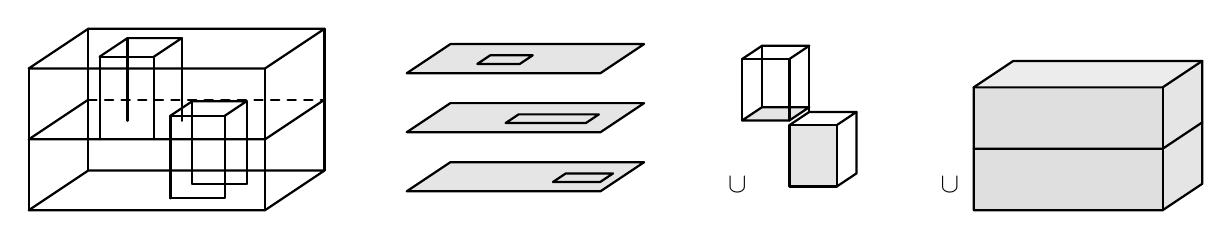
\begin{tikzpicture}[
				scale=0.6,
				line join=round,
				line cap=round,
				thick,
				x={(1cm,0cm)},
				y={(0.42cm,0.28cm)},
				z={(0cm,1cm)}
			]
				% Left: original cubical space
				\begin{scope}
					% Outer box
					\draw (0,0,0) -- (5,0,0) -- (5,3,0) -- (0,3,0) -- cycle;
					\draw (0,0,0) -- (0,0,3);
					\draw (5,0,0) -- (5,0,3);
					\draw (0,3,0) -- (0,3,3);
					\draw (5,3,0) -- (5,3,3);
					\draw (0,0,3) -- (5,0,3) -- (5,3,3) -- (0,3,3) -- cycle;

					% Middle horizontal plane
					\draw (0,0,1.5) -- (5,0,1.5) -- (5,3,1.5);
					\draw[dashed] (0,3,1.5) -- (5,3,1.5);
					\draw (0,0,1.5) -- (0,3,1.5);

					% Upper internal cubical feature
					\draw (1.5,0,1.5) -- (1.5,0,3.25);
					\draw (2.65,0,1.5) -- (2.65,0,3.25);
					\draw (1.5,0,3.25) -- (2.65,0,3.25);
					\draw (1.5,0,3.25) -- (1.5,1.4,3.25)
						-- (2.65,1.4,3.25) -- (2.65,0,3.25);
					\draw (1.5,1.4,3.25) -- (1.5,1.4,1.5);
					\draw (2.65,1.4,3.25) -- (2.65,1.4,1.5);

					% Lower internal cubical feature
					\draw (3.0,0,0.25) -- (4.15,0,0.25) -- (4.15,0,2);
					\draw (3.0,0,0.25) -- (3.0,0,2);
					\draw (3.0,0,2) -- (4.15,0,2);
					\draw (3.0,0,2) -- (3.0,1.1,2)
						-- (4.15,1.1,2) -- (4.15,0,2);
					\draw (3.0,1.1,2) -- (3.0,1.1,0.25);
					\draw (4.15,1.1,2) -- (4.15,1.1,0.25);
					\draw (3.0,1.1,0.25) -- (4.15,1.1,0.25);
				\end{scope}

				% Right: decomposition into three parts
				\begin{scope}[shift={(8,0,0)}]
					% Three parallel sheets with holes
					\foreach \h/\a/\b in {0.4/2.8/3.8,1.65/1.8/3.5,2.9/1.2/2.1} {
						\fill[gray!20] (0,0,\h) -- (4.1,0,\h)
							-- (4.1,2.2,\h) -- (0,2.2,\h) -- cycle;
						\draw (0,0,\h) -- (4.1,0,\h)
							-- (4.1,2.2,\h) -- (0,2.2,\h) -- cycle;
						\draw (\a,0.7,\h) -- (\b,0.7,\h)
							-- (\b,1.35,\h) -- (\a,1.35,\h) -- cycle;
					}
				\end{scope}

				\node at (14.2,1.9) {$\cup$};

				% Central stepped component
				\begin{scope}[shift={(15.1,0,0)}]
					\fill[gray!20] (0,0,1.9) -- (1,0,1.9)
						-- (1,1,1.9) -- (0,1,1.9) -- cycle;
					\draw (0,0,1.9) -- (1,0,1.9) -- (1,1,1.9)
						-- (0,1,1.9) -- cycle;
					\draw (0,0,1.9) -- (0,0,3.2) -- (1,0,3.2)
						-- (1,0,1.9);
					\draw (0,0,3.2) -- (0,1,3.2) -- (1,1,3.2)
						-- (1,0,3.2);
					\draw (0,1,3.2) -- (0,1,1.9);

					\fill[gray!20] (1,0,0.5) rectangle (2,0,1.8);
					\draw (1,0,0.5) -- (2,0,0.5) -- (2,0,1.8)
						-- (1,0,1.8) -- cycle;
					\draw (1,0,1.8) -- (1,1,1.8)
						-- (2,1,1.8) -- (2,0,1.8);
					\draw (2,0,0.5) -- (2,1,0.5) -- (2,1,1.8);
					\draw (1,1,1.8) -- (1,1,3.2);
				\end{scope}

				\node at (18.7,1.9) {$\cup$};

				% Rightmost solid block
				\begin{scope}[shift={(20,0,0)}]
					\fill[gray!25] (0,0,0) -- (4,0,0) -- (4,0,2.6)
						-- (0,0,2.6) -- cycle;
					\fill[gray!15] (0,0,2.6) -- (4,0,2.6)
						-- (4,2,2.6) -- (0,2,2.6) -- cycle;
					\fill[gray!20] (4,0,0) -- (4,2,0)
						-- (4,2,2.6) -- (4,0,2.6) -- cycle;

					\draw (0,0,0) -- (4,0,0) -- (4,2,0)
						-- (4,2,2.6) -- (0,2,2.6)
						-- (0,0,2.6) -- cycle;
					\draw (0,0,2.6) -- (4,0,2.6) -- (4,2,2.6);
					\draw (4,0,0) -- (4,0,2.6);
					\draw (0,0,1.3) -- (4,0,1.3) -- (4,2,1.3);
				\end{scope}
			\end{tikzpicture}
			\caption{Decomposition of the cubical space into horizontal sections,
			connecting components, and a solid block.}
			\label{fig:cubical_decomposition}
		\end{figure}
	\end{example}

	\begin{definition}[Suspension]
		For a topolgical space $X$, the \textbf{suspension} is defined as 
		\begin{equation}
			S(X) \coloneqq \frac{X \times I}{\sim}
		\end{equation}
		where $\sim$ collapses $X \times \{0\}$ to 1 point and $X \times \{1\}$ to another point. 

		\begin{figure}[H]
			\centering
			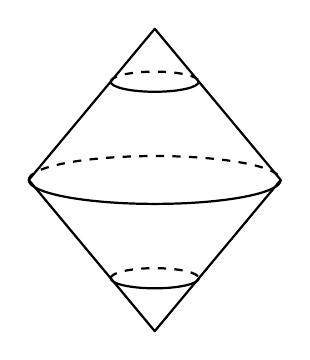
\begin{tikzpicture}[scale=0.8, thick, line join=round]
				% Outer double cone
				\draw (-2,0) -- (0,2.4) -- (2,0) -- (0,-2.4) -- cycle;

				% Middle ellipse
				\draw (-2,0) arc[start angle=180,end angle=360,
					x radius=2,y radius=0.38];
				\draw[dashed] (-2,0) arc[start angle=180,end angle=0,
					x radius=2,y radius=0.38];

				% Upper ellipse
				\draw (-0.7,1.56) arc[start angle=180,end angle=360,
					x radius=0.7,y radius=0.16];
				\draw[dashed] (-0.7,1.56) arc[start angle=180,end angle=0,
					x radius=0.7,y radius=0.16];

				% Lower ellipse
				\draw (-0.7,-1.56) arc[start angle=180,end angle=360,
					x radius=0.7,y radius=0.16];
				\draw[dashed] (-0.7,-1.56) arc[start angle=180,end angle=0,
					x radius=0.7,y radius=0.16];
			\end{tikzpicture}
			\caption{A double cone with horizontal cross-sections.}
			\label{fig:double_cone}
		\end{figure}
	\end{definition} 

\subsection{Popular Topological Spaces}

	Now we unlock a lot of topological spaces. 


	\begin{lemma}[Compact to Hausdorff Criterion]
	  \label{lem:compact_hausdorff_quotient}
		Let $g: X \rightarrow Y$ be a continuous surjection from a compact space $X$ to a Hausdorff space $Y$, and let $x \sim x^\prime \iff g(x) = g(x^\prime)$. Then $X/{\sim} \; \cong Y$. 
	\end{lemma}
	\begin{proof}
	  Closed subsets of $X$ are compact, so their images are compact, hence closed in $Y$. Thus $g$ is a closed map, and a closed continuous surjection is a quotient map. By \hyperref[thm:quotient_homeomorphism]{the universal property of the quotient}, $X/{\sim} \; \cong Y$. 
	\end{proof}

	\begin{definition}[Constructions of the Circle $S^1$]
		The \textbf{1-sphere}, denoted $S^1$, is homeomorphic to all of the spaces below. 
		\begin{enumerate}
			\item \textit{Subspace of $\mathbb{R}^2$}. Given $\mathbb{R}^2$ with the Euclidean topology, 
				\begin{equation}
					S^1 = \{(x, y) \in \mathbb{R}^2 \colon x^2 + y^2 = 1 \}
				\end{equation}
				endowed with the subspace topology. 

					\begin{figure}[H]
					\centering
					\begin{subfigure}[t]{0.48\textwidth}
						\centering
						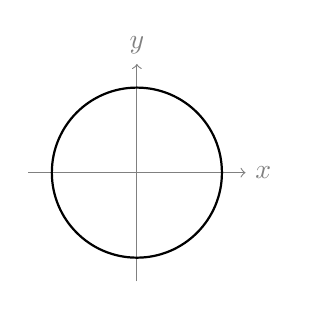
\begin{tikzpicture}[scale=0.6]
							\draw[gray, thin, ->] (-2.3,0) -- (2.3,0) node[right] {$x$};
							\draw[gray, thin, ->] (0,-2.3) -- (0,2.3) node[above] {$y$};
							\draw[thick] (0,0) circle (1.8);
						\end{tikzpicture}
						\caption{The unit circle in the $xy$-plane.}
						\label{fig:s1_r2_circle}
					\end{subfigure}
					\hfill
					\begin{subfigure}[t]{0.48\textwidth}
						\centering
						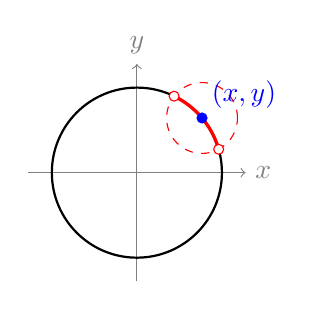
\begin{tikzpicture}[scale=0.6]
							\draw[gray, thin, ->] (-2.3,0) -- (2.3,0) node[right] {$x$};
							\draw[gray, thin, ->] (0,-2.3) -- (0,2.3) node[above] {$y$};
							\draw[thick] (0,0) circle (1.8);
							\draw[dashed, red] (40:1.8) circle (0.75);
							\draw[very thick, red] (64.06:1.8) arc (64.06:15.94:1.8);
							\filldraw[blue] (40:1.8) circle (3pt) node[above right] {$(x, y)$};
							\draw[red, fill=white] (64.06:1.8) circle (3pt);
							\draw[red, fill=white] (15.94:1.8) circle (3pt);
						\end{tikzpicture}
						\caption{Open ball $B_\epsilon((x, y))$ (dashed) around $(x, y) \in S^1$, and the open set $B_\epsilon((x, y)) \cap S^1$ (red arc).}
						\label{fig:s1_r2_open}
					\end{subfigure}
					\caption{Open sets of $S^1 \subset \mathbb{R}^2$ are intersections of open balls of $\mathbb{R}^2$ with the circle.}
					\label{fig:s1_r2}
					\end{figure}

			\item \textit{Subspace of $\mathbb{C}$}. Given $\mathbb{C}$ with the Euclidean topology, 
				\begin{equation}
					S^1 = \{z \in \mathbb{C} \colon |z| = 1 \} 
				\end{equation}
				endowed with the subspace topology. 

					\begin{figure}[H]
					\centering
					\begin{subfigure}[t]{0.48\textwidth}
						\centering
						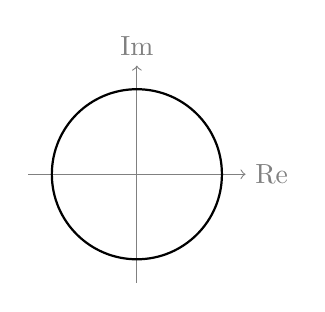
\begin{tikzpicture}[scale=0.6]
							\draw[gray, thin, ->] (-2.3,0) -- (2.3,0) node[right] {$\mathrm{Re}$};
							\draw[gray, thin, ->] (0,-2.3) -- (0,2.3) node[above] {$\mathrm{Im}$};
							\draw[thick] (0,0) circle (1.8);
						\end{tikzpicture}
						\caption{The unit circle in the complex plane.}
						\label{fig:s1_c_circle}
					\end{subfigure}
					\hfill
					\begin{subfigure}[t]{0.48\textwidth}
						\centering
						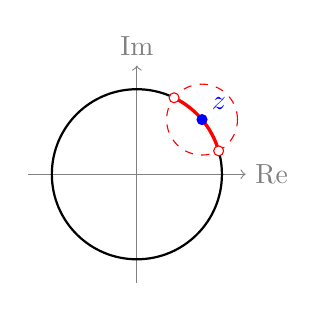
\begin{tikzpicture}[scale=0.6]
							\draw[gray, thin, ->] (-2.3,0) -- (2.3,0) node[right] {$\mathrm{Re}$};
							\draw[gray, thin, ->] (0,-2.3) -- (0,2.3) node[above] {$\mathrm{Im}$};
							\draw[thick] (0,0) circle (1.8);
							\draw[dashed, red] (40:1.8) circle (0.75);
							\draw[very thick, red] (64.06:1.8) arc (64.06:15.94:1.8);
							\filldraw[blue] (40:1.8) circle (3pt) node[above right] {$z$};
							\draw[red, fill=white] (64.06:1.8) circle (3pt);
							\draw[red, fill=white] (15.94:1.8) circle (3pt);
						\end{tikzpicture}
						\caption{Open ball $B_\epsilon(z)$ (dashed) around $z \in S^1$, and the open set $B_\epsilon(z) \cap S^1$ (red arc).}
						\label{fig:s1_c_open}
					\end{subfigure}
					\caption{Open sets of $S^1 \subset \mathbb{C}$ are intersections of open balls of $\mathbb{C}$ with the circle.}
					\label{fig:s1_c}
					\end{figure}

			\item \textit{Quotient of $[0, 1]$}. Given $[0, 1]$, we let $0 \sim 1$ and let
				\begin{equation}
					S^1 = \frac{[0, 1]}{\sim}
				\end{equation}

				\begin{figure}[H]
				\centering
				\begin{subfigure}[t]{0.32\textwidth}
					\centering
					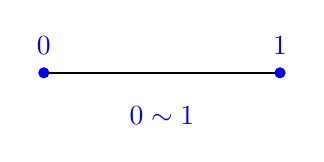
\begin{tikzpicture}[scale=0.6]
						\draw[thick] (0,0) -- (5,0);
						\filldraw[blue] (0,0) circle (3pt) node[above=3pt] {$0$};
						\filldraw[blue] (5,0) circle (3pt) node[above=3pt] {$1$};
						\node[blue] at (2.5,-0.9) {$0 \sim 1$};
					\end{tikzpicture}
					\caption{Space $[0,1]/{\sim}$ with points identified under $\sim$}
					\label{fig:s1_int_ident}
				\end{subfigure}
				\hfill
				\begin{subfigure}[t]{0.32\textwidth}
					\centering
					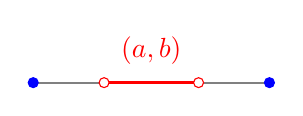
\begin{tikzpicture}[scale=0.6]
						\draw[thick, gray] (0,0) -- (5,0);
						\filldraw[blue] (0,0) circle (3pt);
						\filldraw[blue] (5,0) circle (3pt);
						\draw[very thick, red] (1.5,0) -- (3.5,0);
						\draw[red, fill=white] (1.5,0) circle (3pt);
						\draw[red, fill=white] (3.5,0) circle (3pt);
						\node[red, above=3pt] at (2.5,0) {$(a, b)$};
					\end{tikzpicture}
					\caption{Saturated open sets of $[0,1]/{\sim}$ at an interior point}
					\label{fig:s1_int_interior}
				\end{subfigure}
				\hfill
				\begin{subfigure}[t]{0.32\textwidth}
					\centering
					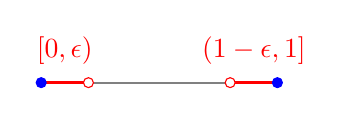
\begin{tikzpicture}[scale=0.6]
						\draw[thick, gray] (0,0) -- (5,0);
						\draw[very thick, red] (0,0) -- (1,0);
						\draw[very thick, red] (4,0) -- (5,0);
						\filldraw[blue] (0,0) circle (3pt);
						\filldraw[blue] (5,0) circle (3pt);
						\draw[red, fill=white] (1,0) circle (3pt);
						\draw[red, fill=white] (4,0) circle (3pt);
						\node[red, above=3pt] at (0.5,0) {$[0, \epsilon)$};
						\node[red, above=3pt] at (4.5,0) {$(1 - \epsilon, 1]$};
					\end{tikzpicture}
					\caption{Saturated open sets of $[0,1]/{\sim}$ at $[0] = [1]$}
					\label{fig:s1_int_endpoint}
				\end{subfigure}
				\caption{Open sets of $[0, 1]/{\sim}$ correspond to saturated open sets of $[0, 1]$. A neighborhood of $[0]$ must contain a neighborhood of both $0$ and $1$.}
				\label{fig:s1_int}
				\end{figure}
			\item \textit{Quotient of $\mathbb{R}$}. Given $\mathbb{R}$ with the Euclidean topology, we let $x \sim y$ iff $x - y \in \mathbb{Z}$ and let 
				\begin{equation}
					S^1 = \frac{\mathbb{R}}{\sim} = \frac{\mathbb{R}}{\mathbb{Z}}
				\end{equation}

				\begin{figure}[H]
				\centering
				\begin{subfigure}[t]{0.32\textwidth}
					\centering
					\begin{tikzpicture}[scale=0.6]
						\draw[thick, <->, >=stealth] (-0.8,0) -- (6.8,0);
		
						\foreach \x/\l in {0/0, 3/1, 6/2} {
						  \draw (\x,0.12) -- (\x,-0.12);
						  \filldraw[blue] (\x,0) circle (3pt) node[above=3pt] {$\l$};
						}
						\foreach \x/\l in {1.5/\tfrac{1}{2}, 4.5/\tfrac{3}{2}} {
						  \filldraw[red] (\x,0) circle (3pt) node[above=3pt] {$\l$};
						}
					\end{tikzpicture}
					\caption{Space $\mathbb{R}/\mathbb{Z}$ with points identified under $\sim$}
					\label{fig:s1_R_ident}
				\end{subfigure}
				\hfill
				\begin{subfigure}[t]{0.32\textwidth}
					\centering
					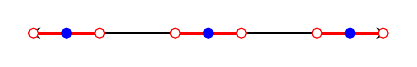
\begin{tikzpicture}[scale=0.6]
						\draw[thick, <->, >=stealth] (-0.8,0) -- (6.8,0);
		
						\foreach \x in {0,3,6} {
						  \draw[very thick, red] (\x-0.7,0) -- (\x+0.7,0);
						  \draw[red, fill=white] (\x-0.7,0) circle (3pt);
						  \draw[red, fill=white] (\x+0.7,0) circle (3pt);
						  \filldraw[blue] (\x,0) circle (3pt);
						}
					\end{tikzpicture}
					\caption{Saturated open sets of $\mathbb{R}/\mathbb{Z}$ at $[0]$}
					\label{fig:s1_R_zero}
				\end{subfigure}
				\hfill
				\begin{subfigure}[t]{0.32\textwidth}
					\centering
					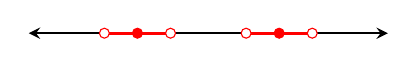
\begin{tikzpicture}[scale=0.6]
						\draw[thick, <->, >=stealth] (-0.8,0) -- (6.8,0);
		
						\foreach \x in {1.5,4.5} {
						  \draw[very thick, red] (\x-0.7,0) -- (\x+0.7,0);
						  \draw[red, fill=white] (\x-0.7,0) circle (3pt);
						  \draw[red, fill=white] (\x+0.7,0) circle (3pt);
						  \filldraw[red] (\x,0) circle (3pt);
						}
					\end{tikzpicture}
					\caption{Saturated open sets of $\mathbb{R}/\mathbb{Z}$ at $[\tfrac{1}{2}]$}
					\label{fig:s1_R_half}
				\end{subfigure}
				\caption{Open sets of $\mathbb{R}/\mathbb{Z}$ correspond to saturated open sets of $\mathbb{R}$, i.e. open sets invariant under translation by $\mathbb{Z}$.}
				\label{fig:s1_R}
				\end{figure}
		\end{enumerate}
	\end{definition}
	\begin{proof}
	  We prove the following. 
		\begin{enumerate}
		  \item $(1) \cong (2)$. The map $\varphi: \mathbb{R}^2 \rightarrow \mathbb{C}$, $\varphi(x, y) = x + iy$ is a homeomorphism (it is an isometry for the Euclidean metrics, since $|x + iy| = \sqrt{x^2 + y^2}$). It maps $\{x^2 + y^2 = 1\}$ bijectively onto $\{|z| = 1\}$, and the restriction of a homeomorphism to a subspace is a homeomorphism onto its image with the subspace topology. 

			\item $(1) \cong (3)$. Our intuition may tell us that by ``sticking'' the endpoints together, we can get a unit circle $S^1$. 

				Define 
				\begin{equation}
					f: [0, 1] \rightarrow S^1, \quad f(x) \coloneqq (\cos{2 \pi x}, \sin{2\pi x})
				\end{equation} 
				It is continuous and surjective, and $f(x) = f(x^\prime) \iff x = x^\prime$ or $\{x, x^\prime\} = \{0, 1\}$, i.e. $\iff x \sim x^\prime$. Since $[0, 1]$ is compact and $S^1$ is Hausdorff, $f$ is a closed map (closed subsets of $[0, 1]$ are compact, so their images are compact and hence closed). A closed continuous surjection is a quotient map, so by \hyperref[thm:quotient_homeomorphism]{the universal property of the quotient}, $[0, 1]/{\sim} \; \cong S^1$ via $\bar{f}([x]) = f(x)$. 

			\item $(2) \cong (4)$. Define 
				\begin{equation}
					q: \mathbb{R} \rightarrow S^1 \subset \mathbb{C}, \quad q(t) \coloneqq e^{2 \pi i t}
				\end{equation}
				It is continuous and surjective, and $q(s) = q(t) \iff s - t \in \mathbb{Z} \iff s \sim t$. We claim $q$ is an open map. Every open set of $\mathbb{R}$ is a union of open intervals of length $\leq 1$, and $q$ maps such an interval $(a, b)$ homeomorphically onto an open arc of $S^1$ (its inverse is a branch of the angle function). Thus $q$ maps open sets to unions of open arcs, which are open. A continuous open surjection is a quotient map, so by \hyperref[thm:quotient_homeomorphism]{the universal property of the quotient}, $\mathbb{R}/\mathbb{Z} \cong S^1$ via $\bar{q}([t]) = e^{2 \pi i t}$. 
		\end{enumerate}

		\textit{Remarks.} Since $[0, 1) \rightarrow \mathbb{R}/\mathbb{Z}$ is a bijection, one may be tempted to replace $S^1$ by $[0, 1)$. However, $\mathbb{R} / \mathbb{Z} \not\cong [0, 1)$: the set $[0, \tfrac{1}{4})$ is open in $[0, 1)$, but its image $\{[x] \colon 0 \leq x < \tfrac{1}{4}\}$ is not open in $\mathbb{R}/\mathbb{Z}$, since its saturation $\bigcup_{n} [n, n + \tfrac{1}{4})$ is not open in $\mathbb{R}$. Also, combining the above with the construction of the torus, 
		\begin{equation}
			S^1 \times S^1 \cong \frac{[0,1]^2}{\sim^\prime} \cong \bigg( \frac{\mathbb{R}}{\mathbb{Z}} \bigg)^2
		\end{equation}
		where $\sim^\prime$ is the relation defined in the construction of the torus. 
	\end{proof}

	\begin{definition}[Constructions of $n$-Sphere $S^n$]
		The \textbf{$n$-sphere}, denoted $S^n$, is homeomorphic to all of the spaces below. 
		\begin{enumerate}
			\item \textit{Subspace of $\mathbb{R}^{n+1}$}. Given $\mathbb{R}^{n+1}$ with the Euclidean topology, 
				\begin{equation}
					S^n = \{x \in \mathbb{R}^{n+1} \colon \|x\| = 1 \}
				\end{equation}
				endowed with the subspace topology.

				\begin{figure}[H]
				\centering
				\begin{subfigure}[t]{0.48\textwidth}
					\centering
					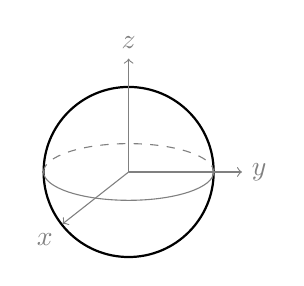
\begin{tikzpicture}[scale=0.6]
						\draw[thick] (0,0) circle (1.8);
						\draw[thin, gray] (-1.8,0) arc (180:360:1.8 and 0.6);
						\draw[thin, gray, dashed] (-1.8,0) arc (180:0:1.8 and 0.6);
						\draw[gray,thin,->] (0,0) -- (2.4,0) node[right] {$y$};
						\draw[gray,thin,->] (0,0) -- (0,2.4) node[above] {$z$};
						\draw[gray,thin,->] (0,0) -- (-1.4,-1.1) node[below left] {$x$};
					\end{tikzpicture}
					\caption{The unit sphere in $\mathbb{R}^3$.}
					\label{fig:s2_sub_a}
				\end{subfigure}
				\hfill
				\begin{subfigure}[t]{0.48\textwidth}
					\centering
					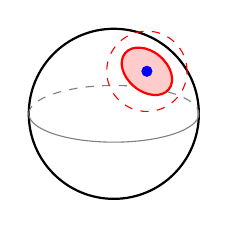
\begin{tikzpicture}[scale=0.6]
						\draw[thick] (0,0) circle (1.8);
						\draw[thin, gray] (-1.8,0) arc (180:360:1.8 and 0.6);
						\draw[thin, gray, dashed] (-1.8,0) arc (180:0:1.8 and 0.6);
						\draw[dashed, red] (0.7,0.9) circle (0.85);
						\draw[red, thick, fill=red!20, rotate around={-40:(0.7,0.9)}] (0.7,0.9) ellipse (0.6 and 0.42);
						\filldraw[blue] (0.7,0.9) circle (3pt) node[above right] {};
					\end{tikzpicture}
					\caption{Open ball (dashed) around $p \in S^2$, and the open set (red cap) which is its intersection with $S^2$.}
					\label{fig:s2_sub_b}
				\end{subfigure}
				\caption{Open sets of $S^2 \subset \mathbb{R}^3$ are intersections of open balls of $\mathbb{R}^3$ with the sphere.}
				\label{fig:s2_sub}
				\end{figure}

			\item \textit{Quotient of $\mathbb{R}^{n+1} \setminus \{0\}$}. We let $x \sim y$ iff $y = \lambda x$ for some $\lambda > 0$ (i.e. they lie on the same open ray from the origin) and let 
				\begin{equation}
					S^n = \frac{\mathbb{R}^{n+1} \setminus \{0\}}{\sim}
				\end{equation}

				\begin{figure}[H]
					\centering
					\begin{subfigure}[t]{0.32\textwidth}
						\centering
						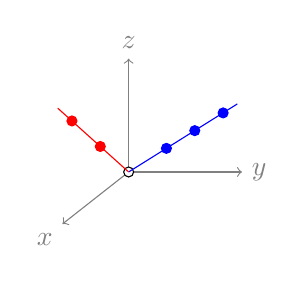
\begin{tikzpicture}[scale=0.6]
							\draw[gray,thin,->] (0,0) -- (2.4,0) node[right] {$y$};
							\draw[gray,thin,->] (0,0) -- (0,2.4) node[above] {$z$};
							\draw[gray,thin,->] (0,0) -- (-1.4,-1.1) node[below left] {$x$};
							\draw[black, fill=white] (0,0) circle (3pt);
							\draw[blue, thin] (0,0) -- (2.3,1.44);
							\filldraw[blue] (0.8,0.5) circle (3pt);
							\filldraw[blue] (1.4000000000000001,0.875) circle (3pt);
							\filldraw[blue] (2.0,1.25) circle (3pt);
							\draw[red, thin] (0,0) -- (-1.5,1.35);
							\filldraw[red] (-0.6,0.54) circle (3pt);
							\filldraw[red] (-1.2,1.08) circle (3pt);
						\end{tikzpicture}
						\caption{Space $(\mathbb{R}^3 \setminus \{0\})/{\sim}$ with points identified under $\sim$}
						\label{fig:s2_rays_a}
					\end{subfigure}
					\hfill
					\begin{subfigure}[t]{0.32\textwidth}
						\centering
						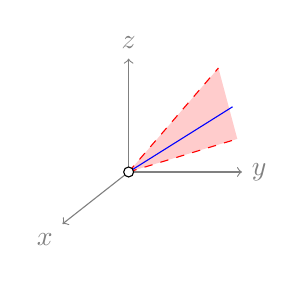
\begin{tikzpicture}[scale=0.6]
							\draw[gray,thin,->] (0,0) -- (2.4,0) node[right] {$y$};
							\draw[gray,thin,->] (0,0) -- (0,2.4) node[above] {$z$};
							\draw[gray,thin,->] (0,0) -- (-1.4,-1.1) node[below left] {$x$};
							\fill[red!20] (0,0) -- (2.3,0.7) -- (1.9,2.2) -- cycle;
							\draw[red, dashed] (0,0) -- (2.3,0.7);
							\draw[red, dashed] (0,0) -- (1.9,2.2);
							\draw[blue, thin] (0,0) -- (2.2,1.38);
							\draw[black, fill=white] (0,0) circle (3pt);
						\end{tikzpicture}
						\caption{Saturated open sets of $(\mathbb{R}^3 \setminus \{0\})/{\sim}$ at a ray}
						\label{fig:s2_rays_b}
					\end{subfigure}
					\hfill
					\begin{subfigure}[t]{0.32\textwidth}
						\centering
						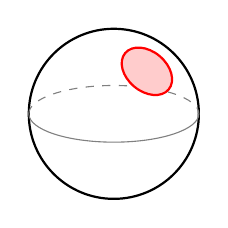
\begin{tikzpicture}[scale=0.6]
							\draw[thick] (0,0) circle (1.8);
							\draw[thin, gray] (-1.8,0) arc (180:360:1.8 and 0.6);
							\draw[thin, gray, dashed] (-1.8,0) arc (180:0:1.8 and 0.6);
							\draw[red, thick, fill=red!20, rotate around={-40:(0.7,0.9)}] (0.7,0.9) ellipse (0.6 and 0.42);
						\end{tikzpicture}
						\caption{Saturated open sets of $(\mathbb{R}^3 \setminus \{0\})/{\sim}$ at a ray, restricted to $S^2$}
						\label{fig:s2_rays_c}
					\end{subfigure}
					\caption{Open sets of $(\mathbb{R}^3 \setminus \{0\})/{\sim}$ are open cones.}
					\label{fig:s2_rays}
				\end{figure}

			\item \textit{Quotient of $D^n$}. Given the closed unit disk $D^n = \{x \in \mathbb{R}^n \colon \|x\| \leq 1\}$, we let $x \sim y$ iff $x = y$ or $x, y \in \partial D^n = S^{n-1}$ and let 
				\begin{equation}
					S^n = \frac{D^n}{\partial D^n} 
				\end{equation}

				\begin{figure}[H]
					\centering
					\begin{subfigure}[t]{0.32\textwidth}
						\centering
						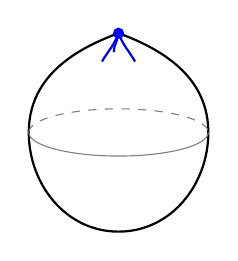
\begin{tikzpicture}[scale=0.6]
						\draw[thick] (0,2.3) to[out=200,in=90] (-1.9,0.2) to[out=270,in=180] (0,-1.9) to[out=0,in=270] (1.9,0.2) to[out=90,in=-20] (0,2.3);
						\draw[thin, gray] (-1.9,0.2) arc (180:360:1.9 and 0.5);
						\draw[thin, gray, dashed] (-1.9,0.2) arc (180:0:1.9 and 0.5);
						\draw[thick, blue] (0,2.3) to[out=-110,in=60] (-0.35,1.7);
						\draw[thick, blue] (0,2.3) to[out=-70,in=120] (0.35,1.7);
						\draw[thick, blue] (0,2.3) to[out=-95,in=90] (-0.1,1.9);
						\filldraw[blue] (0,2.3) circle (3pt);
						\end{tikzpicture}
						\caption{Space $D^2/\partial D^2$ with points identified under $\sim$}
						\label{fig:s2_disk_a}
					\end{subfigure}
					\hfill
					\begin{subfigure}[t]{0.32\textwidth}
						\centering
						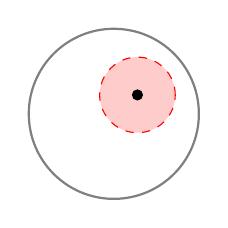
\begin{tikzpicture}[scale=0.6]
							\draw[thick, gray] (0,0) circle (1.8);
							\draw[dashed, red, fill=red!20] (0.5,0.4) circle (0.8);
							\filldraw[black] (0.5,0.4) circle (3pt);
						\end{tikzpicture}
						\caption{Saturated open sets of $D^2/\partial D^2$ at an interior point}
						\label{fig:s2_disk_b}
					\end{subfigure}
					\hfill
					\begin{subfigure}[t]{0.32\textwidth}
						\centering
						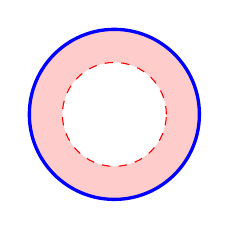
\begin{tikzpicture}[scale=0.6]
							\fill[red!20, even odd rule] (0,0) circle (1.8) (0,0) circle (1.1);
							\draw[red, dashed] (0,0) circle (1.1);
							\draw[very thick, blue] (0,0) circle (1.8);
						\end{tikzpicture}
						\caption{Saturated open sets of $D^2/\partial D^2$ at $[\partial D^2]$}
						\label{fig:s2_disk_c}
					\end{subfigure}
					\caption{Open sets of $D^2/\partial D^2$.}
					\label{fig:s2_disk}
				\end{figure}

			\item \textit{Quotient of $[0, 1]^n$}. Given $[0, 1]^n$, we let $x \sim y$ iff $x = y$ or $x, y \in \partial [0, 1]^n$ and let 
				\begin{equation}
					S^n = \frac{[0, 1]^n}{\partial [0, 1]^n}
				\end{equation}

				\begin{figure}[H]
					\centering
					\begin{subfigure}[t]{0.32\textwidth}
						\centering
						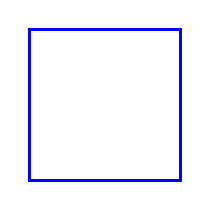
\begin{tikzpicture}[scale=0.6]
							\draw[very thick, blue] (0,0) rectangle (3.2,3.2);
						\end{tikzpicture}
						\caption{Space $[0,1]^2/\partial[0,1]^2$ with points identified under $\sim$}
						\label{fig:s2_cube_a}
					\end{subfigure}
					\hfill
					\begin{subfigure}[t]{0.32\textwidth}
						\centering
						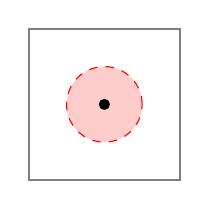
\begin{tikzpicture}[scale=0.6]
							\draw[thick, gray] (0,0) rectangle (3.2,3.2);
							\draw[dashed, red, fill=red!20] (1.6,1.6) circle (0.8);
							\filldraw[black] (1.6,1.6) circle (3pt);
						\end{tikzpicture}
						\caption{Saturated open sets of $[0,1]^2/\sim$ at an interior point}
						\label{fig:s2_cube_b}
					\end{subfigure}
					\hfill
					\begin{subfigure}[t]{0.32\textwidth}
						\centering
						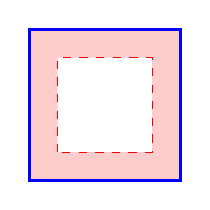
\begin{tikzpicture}[scale=0.6]
							\fill[red!20, even odd rule] (0,0) rectangle (3.2,3.2) (0.6,0.6) rectangle (2.6,2.6);
							\draw[red, dashed] (0.6,0.6) rectangle (2.6,2.6);
							\draw[very thick, blue] (0,0) rectangle (3.2,3.2);
						\end{tikzpicture}
						\caption{Saturated open sets of $[0,1]^2/\sim$ at $[\partial [0,1]^2]$}
						\label{fig:s2_cube_c}
					\end{subfigure}
					\caption{Open sets of $[0,1]^2/\partial[0,1]^2$.}
					\label{fig:s2_cube}
				\end{figure}
		\end{enumerate}
	\end{definition}
	\begin{proof}
		In (3) and (4), we use the following criterion: if $g: X \rightarrow Y$ is a continuous surjection from a compact space to a Hausdorff space, then $g$ is closed (closed subsets of $X$ are compact, so their images are compact, hence closed in $Y$), and a closed continuous surjection is a quotient map. So if in addition $x \sim x^\prime \iff g(x) = g(x^\prime)$, then \hyperref[thm:quotient_homeomorphism]{the universal property of the quotient} gives $X/{\sim} \; \cong Y$. 
		\begin{enumerate}
			\item $(1) \cong (2)$. Let $p: \mathbb{R}^{n+1} \setminus \{0\} \rightarrow (\mathbb{R}^{n+1} \setminus \{0\})/{\sim}$ be the quotient map and let $\pi \coloneqq p|_{S^n}$, which is continuous. It is bijective since every open ray meets $S^n$ in exactly one point. Conversely, define 
				\begin{equation}
					r: \mathbb{R}^{n+1} \setminus \{0\} \rightarrow S^n, \quad r(x) \coloneqq \frac{x}{\|x\|}
				\end{equation}
				which is continuous and satisfies $r(x) = r(y)$ whenever $x \sim y$. By \hyperref[thm:universal_quotient]{the universal property of the quotient}, it descends to a continuous map $\bar{r}: (\mathbb{R}^{n+1} \setminus \{0\})/{\sim} \rightarrow S^n$ with $\bar{r} \circ p = r$. Then $\bar{r} \circ \pi = r|_{S^n} = \mathrm{id}_{S^n}$, and $\pi \circ \bar{r} \circ p = \pi \circ r = p$ since $x \sim r(x)$, so $\pi \circ \bar{r} = \mathrm{id}$ because $p$ is surjective. Hence $\pi$ is a homeomorphism with inverse $\bar{r}$. 

			\item $(1) \cong (3)$. Our intuition may tell us that by squishing the boundary of the disk into a point, we get a sphere. For $n = 2$ this is the following. 


				Define $f: D^n \rightarrow S^n \subset \mathbb{R}^n \times \mathbb{R}$ by 
				\begin{equation}
					f(x) \coloneqq \Big( 2 \sqrt{1 - \|x\|^2} \, x, \; 2\|x\|^2 - 1 \Big)
				\end{equation}
				which is continuous, and lands in $S^n$ since $4(1 - \|x\|^2)\|x\|^2 + (2 \|x\|^2 - 1)^2 = 1$. It is surjective and injective on the interior: given $(v, t) \in S^n$, the last coordinate forces $\|x\|^2 = (1 + t)/2$, and if $t < 1$ then $x = v / (2\sqrt{(1-t)/2})$ is determined uniquely. The only remaining point is $(0, 1)$, which is the image of every $x \in \partial D^n$. Therefore $f(x) = f(x^\prime) \iff x = x^\prime$ or $x, x^\prime \in \partial D^n$, i.e. $x \sim x^\prime$. Since $D^n$ is compact and $S^n$ is Hausdorff, the criterion above gives $D^n/\partial D^n \cong S^n$. 

			\item $(3) \cong (4)$. Define $h: [0, 1]^n \rightarrow D^n$ by $y \coloneqq 2x - 1 \in [-1, 1]^n$ and 
				\begin{equation}
					h(x) \coloneqq \frac{\|y\|_\infty}{\|y\|_2} \, y, \quad h(\tfrac{1}{2}, \ldots, \tfrac{1}{2}) \coloneqq 0
				\end{equation}
				This is a homeomorphism that radially rescales the cube onto the disk, and since $\|h(x)\|_2 = \|y\|_\infty$, it maps $\partial [0, 1]^n$ (where $\|y\|_\infty = 1$) onto $\partial D^n$ and the interior onto the interior. Let $g \coloneqq f \circ h : [0, 1]^n \rightarrow S^n$. It is a continuous surjection, and $g(x) = g(x^\prime)$ iff $h(x) \sim h(x^\prime)$ iff $x = x^\prime$ or $x, x^\prime \in \partial [0, 1]^n$. Since $[0, 1]^n$ is compact, the criterion gives $[0, 1]^n / \partial [0, 1]^n \cong S^n \cong D^n / \partial D^n$. 
		\end{enumerate}
	\end{proof}

	\begin{definition}[Constructions of Real Projective Line $\mathbb{RP}^1$]
		The \textbf{real projective line}, denoted $\mathbb{RP}^1$, is homeomorphic to all of the spaces below. 
		\begin{enumerate}
			\item \textit{Quotient of $\mathbb{R}^2 \setminus \{0\}$}. We let $x \sim y$ iff $y = \lambda x$ for some $\lambda \in \mathbb{R} \setminus \{0\}$ and let 
				\begin{equation}
					\mathbb{RP}^1 = \frac{\mathbb{R}^2 \setminus \{0\}}{\sim}
				\end{equation}

				\begin{figure}[H]
				\centering
				\begin{subfigure}[t]{0.48\textwidth}
					\centering
					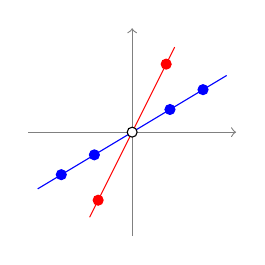
\begin{tikzpicture}[scale=0.6]
						\draw[gray,thin,->] (-2.2,0) -- (2.2,0);
						\draw[gray,thin,->] (0,-2.2) -- (0,2.2);
						\draw[blue, thin] (-2,-1.2) -- (2,1.2);
						\filldraw[blue] (-1.5,-0.8999999999999999) circle (3pt);
						\filldraw[blue] (-0.8,-0.48) circle (3pt);
						\filldraw[blue] (0.8,0.48) circle (3pt);
						\filldraw[blue] (1.5,0.8999999999999999) circle (3pt);
						\draw[red, thin] (-0.9,-1.8) -- (0.9,1.8);
						\filldraw[red] (-0.7200000000000001,-1.4400000000000002) circle (3pt);
						\filldraw[red] (0.7200000000000001,1.4400000000000002) circle (3pt);
						\draw[black, fill=white] (0,0) circle (3pt);
					\end{tikzpicture}
					\caption{Space $(\mathbb{R}^2 \setminus \{0\})/{\sim}$ with points identified under $\sim$}
					\label{fig:rp1_plane_a}
				\end{subfigure}
				\hfill
				\begin{subfigure}[t]{0.48\textwidth}
					\centering
					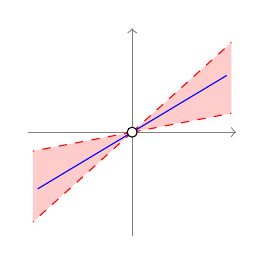
\begin{tikzpicture}[scale=0.6]
						\draw[gray,thin,->] (-2.2,0) -- (2.2,0);
						\draw[gray,thin,->] (0,-2.2) -- (0,2.2);
						\fill[red!20] (0,0) -- (2.1,0.4) -- (2.1,1.9) -- cycle;
						\fill[red!20] (0,0) -- (-2.1,-0.4) -- (-2.1,-1.9) -- cycle;
						\draw[red,dashed] (0,0) -- (2.1,0.4);\draw[red,dashed] (0,0) -- (2.1,1.9);
						\draw[red,dashed] (0,0) -- (-2.1,-0.4);\draw[red,dashed] (0,0) -- (-2.1,-1.9);
						\draw[blue, thin] (-2,-1.2) -- (2,1.2);
						\draw[black, fill=white] (0,0) circle (3pt);
					\end{tikzpicture}
					\caption{Saturated open sets of $(\mathbb{R}^2 \setminus \{0\})/{\sim}$ at a line through the origin}
					\label{fig:rp1_plane_b}
				\end{subfigure}
				\caption{Open sets of $(\mathbb{R}^2 \setminus \{0\})/{\sim}$.}
				\label{fig:rp1_plane}
				\end{figure}

			\item \textit{Quotient of $S^1$}. We let $x \sim y$ iff $y = \pm x$ and let 
				\begin{equation}
					\mathbb{RP}^1 = \frac{S^1}{\sim}
				\end{equation}

				\begin{figure}[H]
				\centering
				\begin{subfigure}[t]{0.48\textwidth}
					\centering
					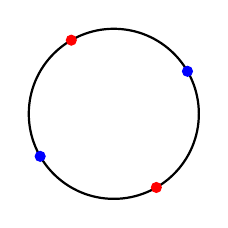
\begin{tikzpicture}[scale=0.6]
						\draw[thick] (0,0) circle (1.8);
						\filldraw[blue] (30:1.8) circle (3pt);
						\filldraw[blue] (210:1.8) circle (3pt);
						\filldraw[red] (120:1.8) circle (3pt);
						\filldraw[red] (300:1.8) circle (3pt);
					\end{tikzpicture}
					\caption{Space $S^1/{\sim}$ with points identified under $\sim$}
					\label{fig:rp1_circle_a}
				\end{subfigure}
				\hfill
				\begin{subfigure}[t]{0.48\textwidth}
					\centering
					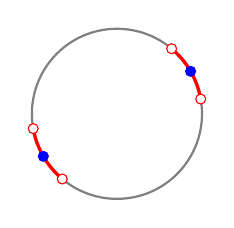
\begin{tikzpicture}[scale=0.6]
						\draw[thick, gray] (0,0) circle (1.8);
						\draw[very thick, red] (50:1.8) arc (50:10:1.8);
						\draw[very thick, red] (230:1.8) arc (230:190:1.8);
						\filldraw[blue] (30:1.8) circle (3pt);
						\filldraw[blue] (210:1.8) circle (3pt);
						\draw[red, fill=white] (50:1.8) circle (3pt);\draw[red, fill=white] (10:1.8) circle (3pt);\draw[red, fill=white] (230:1.8) circle (3pt);\draw[red, fill=white] (190:1.8) circle (3pt);
					\end{tikzpicture}
					\caption{Saturated open sets of $S^1/{\sim}$ at a pair of antipodal points}
					\label{fig:rp1_circle_b}
				\end{subfigure}
				\caption{Open sets of $S^1/{\sim}$.}
				\label{fig:rp1_circle}
				\end{figure}

			\item \textit{Set of 1-Dimensional Linear Subspaces in $\mathbb{R}^2$}. Let $L_1$ be the set of 1-dimensional linear subspaces of $\mathbb{R}^2$, and let $\ell: \mathbb{R}^2 \setminus \{0\} \rightarrow L_1$, $\ell(x) \coloneqq \mathbb{R} x$. We endow $L_1$ with the final topology of $\ell$, i.e. $U \subset L_1$ is open iff $\ell^{-1}(U)$ is open.

				\begin{figure}[H]
				\centering
				\begin{subfigure}[t]{0.48\textwidth}
					\centering
					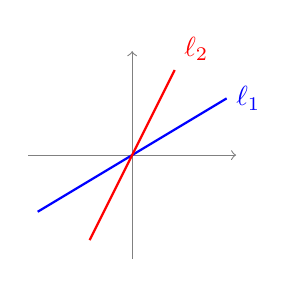
\begin{tikzpicture}[scale=0.6]
						\draw[gray,thin,->] (-2.2,0) -- (2.2,0);
						\draw[gray,thin,->] (0,-2.2) -- (0,2.2);
						\draw[blue, thick] (-2,-1.2) -- (2,1.2);
						\draw[red, thick] (-0.9,-1.8) -- (0.9,1.8);
						\node[blue, right] at (2,1.2) {$\ell_1$};
						\node[red, above right] at (0.9,1.8) {$\ell_2$};
					\end{tikzpicture}
					\caption{Space $L_1$ with points identified under $\sim$}
					\label{fig:rp1_lines_a}
				\end{subfigure}
				\hfill
				\begin{subfigure}[t]{0.48\textwidth}
					\centering
					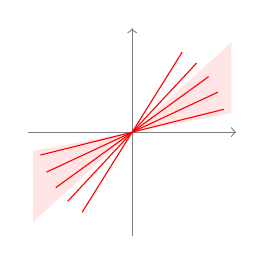
\begin{tikzpicture}[scale=0.6]
						\draw[gray,thin,->] (-2.2,0) -- (2.2,0);
						\draw[gray,thin,->] (0,-2.2) -- (0,2.2);
						\fill[red!10] (0,0) -- (2.1,0.4) -- (2.1,1.9) -- cycle;
						\fill[red!10] (0,0) -- (-2.1,-0.4) -- (-2.1,-1.9) -- cycle;
						\draw[red] (-1.940591452551993,-0.48384379119933546) -- (1.940591452551993,0.48384379119933546);
						\draw[red] (-1.8126155740732999,-0.8452365234813989) -- (1.8126155740732999,0.8452365234813989);
						\draw[red] (-1.618033988749895,-1.1755705045849463) -- (1.618033988749895,1.1755705045849463);
						\draw[red] (-1.363996720124997,-1.462707403238341) -- (1.363996720124997,1.462707403238341);
						\draw[red] (-1.0598385284664098,-1.696096192312852) -- (1.0598385284664098,1.696096192312852);
					\end{tikzpicture}
					\caption{Saturated open sets of $L_1$ at a line through the origin}
					\label{fig:rp1_lines_b}
				\end{subfigure}
				\caption{Open sets of $L_1$.}
				\label{fig:rp1_lines}
				\end{figure}
		\end{enumerate}
	\end{definition}
	\begin{proof}
	  This is the case $n = 1$ of the next definition, whose proof we repeat here. We prove the following. 
		\begin{enumerate}
		  \item $(1) \cong (2)$. Let $r: \mathbb{R}^2 \setminus \{0\} \rightarrow S^1$, $r(x) = x / \|x\|$. It is continuous with continuous right inverse the inclusion $S^1 \hookrightarrow \mathbb{R}^2 \setminus \{0\}$, so it is a quotient map. Composing with the quotient map $p_2: S^1 \rightarrow S^1/{\sim}$ gives a quotient map $q = p_2 \circ r$ with $q(x) = q(y) \iff x \sim y$, so by \hyperref[thm:quotient_homeomorphism]{the universal property of the quotient} the two quotients are homeomorphic. 

			\item $(1) \cong (3)$. The map $\ell$ is surjective with $\ell(x) = \ell(y) \iff x \sim y$, and it is a quotient map by the definition of the topology on $L_1$. By \hyperref[thm:quotient_homeomorphism]{the universal property of the quotient}, $(\mathbb{R}^2 \setminus \{0\})/{\sim} \; \cong L_1$. 
		\end{enumerate}
	\end{proof}

	\begin{definition}[Constructions of Real Projective Space $\mathbb{RP}^n$]
		The \textbf{real projective space}, denoted $\mathbb{RP}^n$, is homeomorphic to all of the spaces below. 
		\begin{enumerate}
			\item \textit{Quotient of $\mathbb{R}^{n+1} \setminus \{0\}$}. We let $x \sim y$ iff $y = \lambda x$ for some $\lambda \in \mathbb{R} \setminus \{0\}$ (i.e. they lie on the same line through the origin) and let 
				\begin{equation}
					\mathbb{RP}^n = \frac{\mathbb{R}^{n+1} \setminus \{0\}}{\sim}
				\end{equation}

				\begin{figure}[H]
				\centering
				\begin{subfigure}[t]{0.48\textwidth}
					\centering
					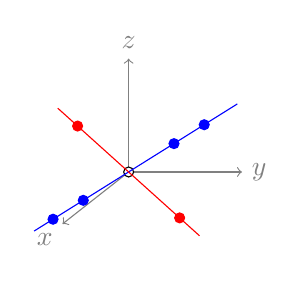
\begin{tikzpicture}[scale=0.6]
						\draw[gray,thin,->] (0,0) -- (2.4,0) node[right] {$y$};
						\draw[gray,thin,->] (0,0) -- (0,2.4) node[above] {$z$};
						\draw[gray,thin,->] (0,0) -- (-1.4,-1.1) node[below left] {$x$};
						\draw[black, fill=white] (0,0) circle (3pt);
						\draw[blue, thin] (-2.0,-1.25) -- (2.3,1.44);
						\filldraw[blue] (-1.6,-1.0) circle (3pt);
						\filldraw[blue] (-0.96,-0.6) circle (3pt);
						\filldraw[blue] (0.96,0.6) circle (3pt);
						\filldraw[blue] (1.6,1.0) circle (3pt);
						\draw[red, thin] (1.5,-1.35) -- (-1.5,1.35);
						\filldraw[red] (1.08,-0.9720000000000001) circle (3pt);
						\filldraw[red] (-1.08,0.9720000000000001) circle (3pt);
					\end{tikzpicture}
					\caption{Space $(\mathbb{R}^3 \setminus \{0\})/{\sim}$ with points identified under $\sim$}
					\label{fig:rpn_space_a}
				\end{subfigure}
				\hfill
				\begin{subfigure}[t]{0.48\textwidth}
					\centering
					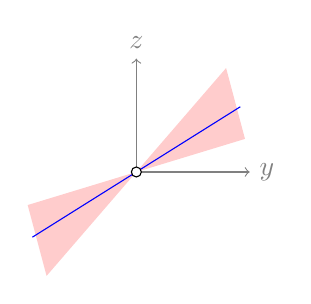
\begin{tikzpicture}[scale=0.6]
						\draw[gray,thin,->] (0,0) -- (2.4,0) node[right] {$y$};
						\draw[gray,thin,->] (0,0) -- (0,2.4) node[above] {$z$};
						\draw[gray,thin,->] (0,0) -- (-1.4,-1.1) node[below left] {$x$};
						\fill[red!20] (0,0) -- (2.3,0.7) -- (1.9,2.2) -- cycle;
						\fill[red!20] (0,0) -- (-2.3,-0.7) -- (-1.9,-2.2) -- cycle;
						\draw[blue, thin] (-2.2,-1.38) -- (2.2,1.38);
						\draw[black, fill=white] (0,0) circle (3pt);
					\end{tikzpicture}
					\caption{Saturated open sets of $(\mathbb{R}^3 \setminus \{0\})/{\sim}$ at a line through the origin}
					\label{fig:rpn_space_b}
				\end{subfigure}
				\caption{Open sets of $(\mathbb{R}^3 \setminus \{0\})/{\sim}$.}
				\label{fig:rpn_space}
				\end{figure}

			\item \textit{Quotient of $S^n$.} We let $x \sim y$ iff $y = \pm x$ and let 
				\begin{equation}
					\mathbb{RP}^n = \frac{S^n}{\sim}
				\end{equation}

				\begin{figure}[H]
				\centering
				\begin{subfigure}[t]{0.48\textwidth}
					\centering
					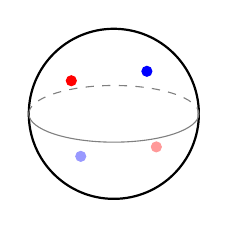
\begin{tikzpicture}[scale=0.6]
						\draw[thick] (0,0) circle (1.8);
						\draw[thin, gray] (-1.8,0) arc (180:360:1.8 and 0.6);
						\draw[thin, gray, dashed] (-1.8,0) arc (180:0:1.8 and 0.6);
						\filldraw[blue] (0.7,0.9) circle (3pt);
						\filldraw[blue!40] (-0.7,-0.9) circle (3pt);
						\filldraw[red] (-0.9,0.7) circle (3pt);
						\filldraw[red!40] (0.9,-0.7) circle (3pt);
					\end{tikzpicture}
					\caption{Space $S^2/{\sim}$ with points identified under $\sim$}
					\label{fig:rpn_sphere_a}
				\end{subfigure}
				\hfill
				\begin{subfigure}[t]{0.48\textwidth}
					\centering
					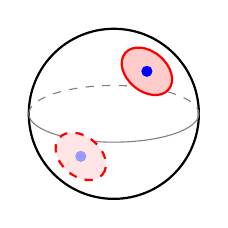
\begin{tikzpicture}[scale=0.6]
						\draw[thick] (0,0) circle (1.8);
						\draw[thin, gray] (-1.8,0) arc (180:360:1.8 and 0.6);
						\draw[thin, gray, dashed] (-1.8,0) arc (180:0:1.8 and 0.6);
						\draw[red, thick, fill=red!20, rotate around={-40:(0.7,0.9)}] (0.7,0.9) ellipse (0.6 and 0.42);
						\draw[red, thick, dashed, fill=red!10, rotate around={-40:(-0.7,-0.9)}] (-0.7,-0.9) ellipse (0.6 and 0.42);
						\filldraw[blue] (0.7,0.9) circle (3pt);
						\filldraw[blue!40] (-0.7,-0.9) circle (3pt);
					\end{tikzpicture}
					\caption{Saturated open sets of $S^2/{\sim}$ at a pair of antipodal points}
					\label{fig:rpn_sphere_b}
				\end{subfigure}
				\caption{Open sets of $S^2/{\sim}$.}
				\label{fig:rpn_sphere}
				\end{figure}

			\item \textit{Set of 1-Dimensional Linear Subspaces in $\mathbb{R}^{n+1}$}. Let $L_n$ be the set of 1-dimensional linear subspaces of $\mathbb{R}^{n+1}$, and let $\ell: \mathbb{R}^{n+1} \setminus \{0\} \rightarrow L_n$, $\ell(x) \coloneqq \mathbb{R} x$. We endow $L_n$ with the final topology of $\ell$, i.e. $U \subset L_n$ is open iff $\ell^{-1}(U)$ is open.

				\begin{figure}[H]
				\centering
				\begin{subfigure}[t]{0.48\textwidth}
					\centering
					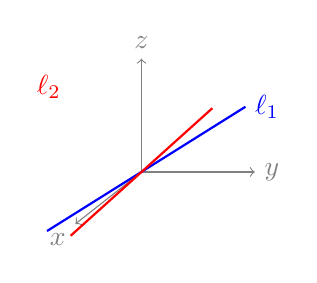
\begin{tikzpicture}[scale=0.6]
						\draw[gray,thin,->] (0,0) -- (2.4,0) node[right] {$y$};
						\draw[gray,thin,->] (0,0) -- (0,2.4) node[above] {$z$};
						\draw[gray,thin,->] (0,0) -- (-1.4,-1.1) node[below left] {$x$};
						\draw[blue, thick] (-2.0,-1.25) -- (2.2,1.38);
						\draw[red, thick] (-1.5,-1.35) -- (1.5,1.35);
						\node[blue, right] at (2.2,1.38) {$\ell_1$};
						\node[red, above left] at (-1.5,1.35) {$\ell_2$};
					\end{tikzpicture}
					\caption{Space $L_2$ with points identified under $\sim$}
					\label{fig:rpn_lines_a}
				\end{subfigure}
				\hfill
				\begin{subfigure}[t]{0.48\textwidth}
					\centering
					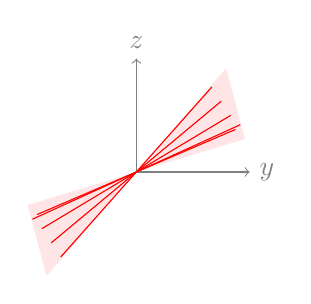
\begin{tikzpicture}[scale=0.6]
						\draw[gray,thin,->] (0,0) -- (2.4,0) node[right] {$y$};
						\draw[gray,thin,->] (0,0) -- (0,2.4) node[above] {$z$};
						\draw[gray,thin,->] (0,0) -- (-1.4,-1.1) node[below left] {$x$};
						\fill[red!10] (0,0) -- (2.3,0.7) -- (1.9,2.2) -- cycle;
						\fill[red!10] (0,0) -- (-2.3,-0.7) -- (-1.9,-2.2) -- cycle;
						\draw[red] (-2.1,-0.9) -- (2.1,0.9);
						\draw[red] (-2.0,-1.2) -- (2.0,1.2);
						\draw[red] (-1.8,-1.5) -- (1.8,1.5);
						\draw[red] (-2.2,-1.0) -- (2.2,1.0);
						\draw[red] (-1.6,-1.8) -- (1.6,1.8);
					\end{tikzpicture}
					\caption{Saturated open sets of $L_2$ at a line through the origin}
					\label{fig:rpn_lines_b}
				\end{subfigure}
				\caption{Open sets of $L_2$.}
				\label{fig:rpn_lines}
				\end{figure}
		\end{enumerate}
	\end{definition}
	\begin{proof}
	  We prove the following. 
		\begin{enumerate}
		  \item $(1) \cong (2)$. Let $r: \mathbb{R}^{n+1} \setminus \{0\} \rightarrow S^n$, $r(x) = x / \|x\|$, which is continuous and has the continuous right inverse given by the inclusion $\iota: S^n \hookrightarrow \mathbb{R}^{n+1} \setminus \{0\}$, so $r$ is a quotient map. Let $p_2: S^n \rightarrow S^n / {\sim}$ be the quotient map. Then $q \coloneqq p_2 \circ r$ is a composition of quotient maps and hence a quotient map. Moreover $q(x) = q(y) \iff r(x) = \pm r(y) \iff y = \lambda x$ for some $\lambda \neq 0 \iff x \sim y$. By \hyperref[thm:quotient_homeomorphism]{the universal property of the quotient}, $(\mathbb{R}^{n+1} \setminus \{0\})/{\sim} \; \cong S^n/{\sim}$. 

			\item $(1) \cong (3)$. The map $\ell$ is surjective, and $\ell(x) = \ell(y) \iff y = \lambda x$ for some $\lambda \neq 0 \iff x \sim y$. By the definition of the topology on $L_n$, $\ell$ is a quotient map. Then by \hyperref[thm:quotient_homeomorphism]{the universal property of the quotient}, $(\mathbb{R}^{n+1} \setminus \{0\})/{\sim} \; \cong L_n$. 
		\end{enumerate}
	\end{proof}

	\begin{definition}[Constructions of the Annulus/Cylinder]
	  The \textbf{annulus/cylinder} is homeomorphic to all of the spaces below. 
		\begin{enumerate}
			\item \textit{Subspace of $\mathbb{R}^2$}. We claim that for $0 < a < b$
				\begin{equation}
					\{(x, y) \in \mathbb{R}^2 \colon a \leq x^2 + y^2 \leq b \}
				\end{equation}

				\begin{figure}[H]
					\centering
					\begin{subfigure}[t]{0.48\textwidth}
						\centering
						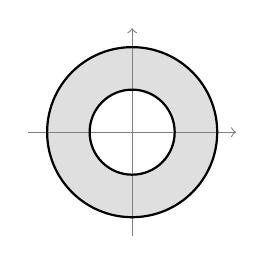
\begin{tikzpicture}[scale=0.6]
							\fill[gray!25, even odd rule] (0,0) circle (1.8) (0,0) circle (0.9);
							\draw[gray,thin,->] (-2.2,0) -- (2.2,0);
							\draw[gray,thin,->] (0,-2.2) -- (0,2.2);
							\draw[thick] (0,0) circle (1.8);
							\draw[thick] (0,0) circle (0.9);
						\end{tikzpicture}
						\caption{The closed annulus in the $xy$-plane.}
						\label{fig:ann_r2_a}
					\end{subfigure}
					\hfill
					\begin{subfigure}[t]{0.48\textwidth}
						\centering
						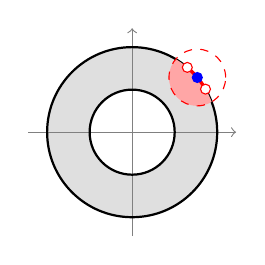
\begin{tikzpicture}[scale=0.6]
							\fill[gray!25, even odd rule] (0,0) circle (1.8) (0,0) circle (0.9);
							\draw[gray,thin,->] (-2.2,0) -- (2.2,0);
							\draw[gray,thin,->] (0,-2.2) -- (0,2.2);
							\draw[thick] (0,0) circle (1.8);
							\draw[thick] (0,0) circle (0.9);
							\begin{scope}\clip (0,0) circle (1.8);\fill[red!35] (40:1.8) circle (0.6);\end{scope}
							\draw[red, dashed] (40:1.8) circle (0.6);
							\draw[red, very thick] (1.167,1.371) arc (49.59406822686046:30.40593177313954:1.8);
							\draw[red, fill=white] (1.167,1.371) circle (3pt);
							\draw[red, fill=white] (1.552,0.911) circle (3pt);
							\filldraw[blue] (40:1.8) circle (3pt);
						\end{tikzpicture}
						\caption{Open ball around a boundary point $p$, and the open set (red) which is its intersection with the annulus.}
						\label{fig:ann_r2_b}
					\end{subfigure}
					\caption{Open sets of the annulus are intersections of open balls of $\mathbb{R}^2$ with it.}
					\label{fig:ann_r2}
				\end{figure}

			\item \textit{Subspace of $\mathbb{R}^3$}. $0 < r, h$
				\begin{equation}
					\{(x, y, z) \in \mathbb{R}^3 \colon x^2 + y^2 = r^2, 0 \leq z \leq h \}
				\end{equation}

				\begin{figure}[H]
					\centering
					\begin{subfigure}[t]{0.48\textwidth}
						\centering
						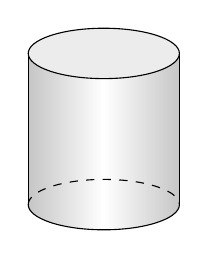
\begin{tikzpicture}[scale=0.8]
							\shade[left color=gray!45, right color=gray!45, middle color=white] (-1.2,2.4) -- (-1.2,0) arc (180:360:1.2 and 0.4) -- (1.2,2.4) -- cycle;
							\draw (-1.2,0) -- (-1.2,2.4);
							\draw (1.2,0) -- (1.2,2.4);
							\draw (-1.2,0) arc (180:360:1.2 and 0.4);
							\draw[dashed] (-1.2,0) arc (180:0:1.2 and 0.4);
							\draw[fill=gray!15] (0,2.4) ellipse (1.2 and 0.4);
						\end{tikzpicture}
						\caption{The cylinder in $\mathbb{R}^3$.}
						\label{fig:ann_r3_a}
					\end{subfigure}
					\hfill
					\begin{subfigure}[t]{0.48\textwidth}
						\centering
						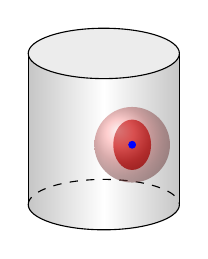
\begin{tikzpicture}[scale=0.8]
							\shade[left color=gray!45, right color=gray!45, middle color=white] (-1.2,2.4) -- (-1.2,0) arc (180:360:1.2 and 0.4) -- (1.2,2.4) -- cycle;
							\draw (-1.2,0) -- (-1.2,2.4);
							\draw (1.2,0) -- (1.2,2.4);
							\draw (-1.2,0) arc (180:360:1.2 and 0.4);
							\draw[dashed] (-1.2,0) arc (180:0:1.2 and 0.4);
							\draw[fill=gray!15] (0,2.4) ellipse (1.2 and 0.4);
							\fill[red!70!black] (0.45,0.95) ellipse (0.3 and 0.4);
							\shade[ball color=red!50, opacity=0.5] (0.45,0.95) circle (0.6);
							\filldraw[blue] (0.45,0.95) circle (1.5pt);
						\end{tikzpicture}
						\caption{Open ball around $p$, and the open set (red) which is its intersection with the cylinder.}
						\label{fig:ann_r3_b}
					\end{subfigure}
					\caption{Open sets of the cylinder are intersections of open balls of $\mathbb{R}^3$ with it.}
					\label{fig:ann_r3}
				\end{figure}

			\item \textit{Quotient of $[0, 1]^2$}. Let $(0, y) \sim (1, y)$ for all $y \in [0, 1]$. Then 
				\begin{equation}
						\frac{[0, 1]^2}{\sim}
				\end{equation}

				\begin{figure}[H]
					\centering
					\begin{subfigure}[t]{0.32\textwidth}
						\centering
						\begin{tikzpicture}[scale=0.7]
							\draw[thick] (0,0) rectangle (3,3);
							\node[rotate=90] at (0,1.5) {$>>$};
							\node[rotate=90] at (3,1.5) {$>>$};
							\filldraw[blue] (0,1) circle (3pt);
							\filldraw[blue] (3,1) circle (3pt);
							\filldraw[red] (0,2.1) circle (3pt);
							\filldraw[red] (3,2.1) circle (3pt);
						\end{tikzpicture}
						\caption{Space $[0,1]^2/{\sim}$ with points identified under $\sim$}
						\label{fig:ann_sq_a}
					\end{subfigure}
					\hfill
					\begin{subfigure}[t]{0.32\textwidth}
						\centering
						\begin{tikzpicture}[scale=0.7]
							\draw[thick] (0,0) rectangle (3,3);
							\draw[dashed, red, fill=red!25] (1.5,1.5) circle (0.7);
							\filldraw[black] (1.5,1.5) circle (3pt);
						\end{tikzpicture}
						\caption{Saturated open sets of $[0,1]^2/{\sim}$ at an interior point}
						\label{fig:ann_sq_b}
					\end{subfigure}
					\hfill
					\begin{subfigure}[t]{0.32\textwidth}
						\centering
						\begin{tikzpicture}[scale=0.7]
							\draw[thick] (0,0) rectangle (3,3);
							\fill[red!25] (0,1) -- ++(-90:0.55) arc (-90:90:0.55) -- cycle;
							\draw[red, dashed] (0,1) ++(-90:0.55) arc (-90:90:0.55);
							\draw[red, thick] (0,1) -- ++(-90:0.55);
							\draw[red, thick] (0,1) -- ++(90:0.55);
							\fill[red!25] (3,1) -- ++(90:0.55) arc (90:270:0.55) -- cycle;
							\draw[red, dashed] (3,1) ++(90:0.55) arc (90:270:0.55);
							\draw[red, thick] (3,1) -- ++(90:0.55);
							\draw[red, thick] (3,1) -- ++(270:0.55);
							\filldraw[blue] (0,1) circle (3pt);
							\filldraw[blue] (3,1) circle (3pt);
						\end{tikzpicture}
						\caption{Saturated open sets of $[0,1]^2/{\sim}$ at an edge point}
						\label{fig:ann_sq_c}
					\end{subfigure}
					\caption{Open sets of $[0,1]^2/{\sim}$ (annulus).}
					\label{fig:ann_sq}
				\end{figure}
		\end{enumerate}
	\end{definition}
	\begin{proof}
	  We prove the following. 
		\begin{enumerate}
		  \item $(1) \cong (2)$. Define $\varphi: \{a \leq \sqrt{x^2 + y^2} \leq b\} \rightarrow \{x^2 + y^2 = r^2, \, 0 \leq z \leq h\}$ by 
				\begin{equation}
					\varphi(x, y) \coloneqq \Big( \frac{r x}{\sqrt{x^2 + y^2}}, \; \frac{r y}{\sqrt{x^2 + y^2}}, \; \frac{h(\sqrt{x^2 + y^2} - a)}{b - a} \Big)
				\end{equation}
				which is continuous since $\sqrt{x^2 + y^2} \geq a > 0$. Its inverse is 
				\begin{equation}
					\psi(X, Y, Z) \coloneqq \Big( a + \frac{(b - a) Z}{h} \Big) \frac{(X, Y)}{r}
				\end{equation}
				which is continuous. Since $\sqrt{X^2 + Y^2} = r$ on the cylinder, $\psi$ rescales $(X, Y)$ to radius $\rho = a + (b-a)Z/h$, and $\varphi$ then sends this back to $(X, Y, Z)$. Similarly $\psi \circ \varphi = \mathrm{id}$. So $\varphi$ is a homeomorphism. 

			\item $(1) \cong (3)$. Our intuition may tell us that by sticking the left and right sides of the square together, we get a cylinder. Define 
				\begin{equation}
					g: [0, 1]^2 \rightarrow \mathbb{R}^2, \quad g(x, y) \coloneqq \big(a + (b - a) y\big) (\cos 2\pi x, \sin 2\pi x)
				\end{equation}
				It is continuous with image the annulus in (1). The radius of $g(x, y)$ determines $y$ (as $a > 0$) and then its angle determines $x$ modulo $1$, so $g(x, y) = g(x^\prime, y^\prime) \iff y = y^\prime$ and $x \equiv x^\prime \pmod 1 \iff (x, y) \sim (x^\prime, y^\prime)$. Since $[0, 1]^2$ is compact and $\mathbb{R}^2$ is Hausdorff, by \hyperref[lem:compact_hausdorff_quotient]{the compact-to-Hausdorff criterion} the quotient is homeomorphic to the annulus. 
		\end{enumerate}
	\end{proof}

	\begin{definition}[Constructions of the Torus]
	  The \textbf{torus}, denoted $T^2$, is homeomorphic to all of the spaces below. 
		\begin{enumerate}
			\item \textit{Subspace of $\mathbb{R}^3$}. It is the subspace 
				\begin{equation}
					\{(x, y, z) \in \mathbb{R}^3 \colon \big( \sqrt{x^2 + y^2} - 2 \big)^2 + z^2 = 1 \}
				\end{equation}

				\begin{figure}[H]
					\centering
					\begin{subfigure}[t]{0.48\textwidth}
						\centering
						\begin{tikzpicture}[scale=0.8]
							\draw (0,0) ellipse (2 and 1.25);
							\draw (-1.05,0.1) .. controls (-0.45,-0.55) and (0.45,-0.55) .. (1.05,0.1);
							\draw (-0.8,-0.02) .. controls (-0.4,0.42) and (0.4,0.42) .. (0.8,-0.02);
						\end{tikzpicture}
						\caption{The torus in $\mathbb{R}^3$.}
						\label{fig:tor_r3_a}
					\end{subfigure}
					\hfill
					\begin{subfigure}[t]{0.48\textwidth}
						\centering
						\begin{tikzpicture}[scale=0.8]
							\draw (0,0) ellipse (2 and 1.25);
							\draw (-1.05,0.1) .. controls (-0.45,-0.55) and (0.45,-0.55) .. (1.05,0.1);
							\draw (-0.8,-0.02) .. controls (-0.4,0.42) and (0.4,0.42) .. (0.8,-0.02);
							\fill[red!70!black] (0.85,-0.8) ellipse (0.38 and 0.24);
							\shade[ball color=red!50, opacity=0.5] (0.85,-0.8) circle (0.7);
							\filldraw[blue] (0.85,-0.8) circle (1.5pt);
						\end{tikzpicture}
						\caption{Open ball (light red) around $p$, and the open set (dark red) which is its intersection with the torus.}
						\label{fig:tor_r3_b}
					\end{subfigure}
					\caption{Open sets of the torus are intersections of open balls of $\mathbb{R}^3$ with it.}
					\label{fig:tor_r3}
				\end{figure}

			\item \textit{Quotient of $[0, 1]^2$}. On $[0, 1]^2$, let us define the equivalence relation as $(0, y) \sim (1, y)$ for $y \in [0, 1]$ and $(x, 0) \sim (x, 1)$ for $x \in [0, 1]$. 
				\begin{equation}
					T^2 \cong \frac{[0, 1]^2}{\sim}
				\end{equation}

				\begin{figure}[H]
					\centering
					\begin{subfigure}[t]{0.32\textwidth}
						\centering
						\begin{tikzpicture}[scale=0.7]
							\draw[thick] (0,0) rectangle (3,3);
							\node at (1.5,3) {$>$};
							\node at (1.5,0) {$>$};
							\node[rotate=90] at (0,1.5) {$>>$};
							\node[rotate=90] at (3,1.5) {$>>$};
							\filldraw[blue] (0,2.2) circle (3pt);
							\filldraw[blue] (3,2.2) circle (3pt);
							\filldraw[red] (2.2,0) circle (3pt);
							\filldraw[red] (2.2,3) circle (3pt);
							\filldraw[violet] (0,0) circle (3pt);
							\filldraw[violet] (3,0) circle (3pt);
							\filldraw[violet] (0,3) circle (3pt);
							\filldraw[violet] (3,3) circle (3pt);
						\end{tikzpicture}
						\caption{Space $[0,1]^2/{\sim}$ with points identified under $\sim$}
						\label{fig:tor_sq_a}
					\end{subfigure}
					\hfill
					\begin{subfigure}[t]{0.32\textwidth}
						\centering
						\begin{tikzpicture}[scale=0.7]
							\draw[thick] (0,0) rectangle (3,3);
							\fill[red!25] (0,2.2) -- ++(-90:0.55) arc (-90:90:0.55) -- cycle;
							\draw[red, dashed] (0,2.2) ++(-90:0.55) arc (-90:90:0.55);
							\draw[red, thick] (0,2.2) -- ++(-90:0.55);
							\draw[red, thick] (0,2.2) -- ++(90:0.55);
							\fill[red!25] (3,2.2) -- ++(90:0.55) arc (90:270:0.55) -- cycle;
							\draw[red, dashed] (3,2.2) ++(90:0.55) arc (90:270:0.55);
							\draw[red, thick] (3,2.2) -- ++(90:0.55);
							\draw[red, thick] (3,2.2) -- ++(270:0.55);
							\filldraw[blue] (0,2.2) circle (3pt);
							\filldraw[blue] (3,2.2) circle (3pt);
						\end{tikzpicture}
						\caption{Saturated open sets of $[0,1]^2/{\sim}$ at an edge point}
						\label{fig:tor_sq_b}
					\end{subfigure}
					\hfill
					\begin{subfigure}[t]{0.32\textwidth}
						\centering
						\begin{tikzpicture}[scale=0.7]
							\draw[thick] (0,0) rectangle (3,3);
							\fill[red!25] (0,0) -- ++(0:0.55) arc (0:90:0.55) -- cycle;
							\draw[red, dashed] (0,0) ++(0:0.55) arc (0:90:0.55);
							\draw[red, thick] (0,0) -- ++(0:0.55);
							\draw[red, thick] (0,0) -- ++(90:0.55);
							\fill[red!25] (3,0) -- ++(90:0.55) arc (90:180:0.55) -- cycle;
							\draw[red, dashed] (3,0) ++(90:0.55) arc (90:180:0.55);
							\draw[red, thick] (3,0) -- ++(90:0.55);
							\draw[red, thick] (3,0) -- ++(180:0.55);
							\fill[red!25] (3,3) -- ++(180:0.55) arc (180:270:0.55) -- cycle;
							\draw[red, dashed] (3,3) ++(180:0.55) arc (180:270:0.55);
							\draw[red, thick] (3,3) -- ++(180:0.55);
							\draw[red, thick] (3,3) -- ++(270:0.55);
							\fill[red!25] (0,3) -- ++(270:0.55) arc (270:360:0.55) -- cycle;
							\draw[red, dashed] (0,3) ++(270:0.55) arc (270:360:0.55);
							\draw[red, thick] (0,3) -- ++(270:0.55);
							\draw[red, thick] (0,3) -- ++(360:0.55);
							\filldraw[violet] (0,0) circle (3pt);
							\filldraw[violet] (3,0) circle (3pt);
							\filldraw[violet] (0,3) circle (3pt);
							\filldraw[violet] (3,3) circle (3pt);
						\end{tikzpicture}
						\caption{Saturated open sets of $[0,1]^2/{\sim}$ at the corner point}
						\label{fig:tor_sq_c}
					\end{subfigure}
					\caption{Open sets of $[0,1]^2/{\sim}$ (torus).}
					\label{fig:tor_sq}
				\end{figure}
		\end{enumerate}
	\end{definition}
	\begin{proof}
	  We prove the following. 
		\begin{enumerate}
		  \item $(1) \cong (2)$. Our intuition may tell us that by first sticking the sides together, we get a cylinder, and by sticking the top with the bottom, we get a torus. Define 
				\begin{equation}
					f: [0, 1]^2 \rightarrow \mathbb{R}^3, \quad f(x, y) \coloneqq \big( (2 + \cos{2 \pi x}) \cos{2\pi y}, \; (2 + \cos{2 \pi x}) \sin{2 \pi y}, \; \sin{2 \pi x} \big)
				\end{equation}
				It lands in the torus of (1) since $\sqrt{X^2 + Y^2} = 2 + \cos 2\pi x$, so $(\sqrt{X^2 + Y^2} - 2)^2 + Z^2 = \cos^2 2\pi x + \sin^2 2\pi x = 1$. It is surjective: if $(X, Y, Z)$ is on the torus, then $(\sqrt{X^2 + Y^2} - 2, Z)$ lies on the unit circle, so it equals $(\cos 2\pi x, \sin 2\pi x)$ for some $x$, and since $\sqrt{X^2 + Y^2} > 0$ we can write $(X, Y) = \sqrt{X^2 + Y^2} (\cos 2\pi y, \sin 2\pi y)$ for some $y$. Finally, $f(x, y) = f(x^\prime, y^\prime)$ iff $x \equiv x^\prime$ and $y \equiv y^\prime \pmod 1$, since $2\pi x$ is determined by $(\sqrt{X^2 + Y^2} - 2, Z)$ and $2\pi y$ by $(X, Y)$. For $x, x^\prime, y, y^\prime \in [0, 1]$ this holds iff $(x, y) \sim (x^\prime, y^\prime)$ (the four corners are all identified). 


				Since $[0, 1]^2$ is compact and $\mathbb{R}^3$ is Hausdorff, by \hyperref[lem:compact_hausdorff_quotient]{the compact-to-Hausdorff criterion} the quotient is homeomorphic to the torus in (1). 
		\end{enumerate}
	\end{proof}

	\begin{definition}[Constructions of the Mobius Strip]
	  The \textbf{Mobius strip}, denoted $M_1$, is homeomorphic to all of the spaces below. 
		\begin{enumerate}
			\item \textit{Subspace of $\mathbb{R}^3$}. It is the image of $[0, 2\pi] \times [-\tfrac{1}{2}, \tfrac{1}{2}]$ under
				\begin{equation}
					G(\theta, t) \coloneqq \Big( \big(1 + t \cos \tfrac{\theta}{2}\big) \cos \theta, \; \big(1 + t \cos \tfrac{\theta}{2}\big) \sin \theta, \; t \sin \tfrac{\theta}{2} \Big)
				\end{equation}

				\begin{figure}[H]
					\centering
					\begin{subfigure}[t]{0.48\textwidth}
						\centering
						\begin{tikzpicture}[scale=0.7]
						\begin{axis}[
						hide axis,
						view={40}{40}
						]
						\addplot3 [
						surf, shader=faceted interp,
						colormap/blackwhite,
						point meta=x,
						samples=40,
						samples y=5,
						z buffer=sort,
						domain=0:360,
						y domain=-0.5:0.5
						] (
						{(1+0.5*y*cos(x/2))*cos(x)},
						{(1+0.5*y*cos(x/2))*sin(x)},
						{0.5*y*sin(x/2)});
		
						\addplot3 [
						samples=50,
						domain=-145:180, % The domain needs to be adjusted manually, depending on the camera angle, unfortunately
						samples y=0,
						thick
						] (
						{cos(x)},
						{sin(x)},
						{0});
						\end{axis}
						\end{tikzpicture}
						\caption{The M\"obius strip in $\mathbb{R}^3$.}
						\label{fig:mob_r3_a}
					\end{subfigure}
					\hfill
					\begin{subfigure}[t]{0.48\textwidth}
						\centering
						\begin{tikzpicture}[scale=0.7]
						\begin{axis}[
						hide axis,
						view={40}{40}
						]
						\addplot3 [
						surf, shader=faceted interp,
						colormap/blackwhite,
						point meta=x,
						samples=40,
						samples y=5,
						z buffer=sort,
						domain=0:360,
						y domain=-0.5:0.5
						] (
						{(1+0.5*y*cos(x/2))*cos(x)},
						{(1+0.5*y*cos(x/2))*sin(x)},
						{0.5*y*sin(x/2)});
		
						\addplot3 [
						samples=50,
						domain=-145:180, % The domain needs to be adjusted manually, depending on the camera angle, unfortunately
						samples y=0,
						thick
						] (
						{cos(x)},
						{sin(x)},
						{0});
						\addplot3 [surf, shader=flat, colormap={r}{color=(red) color=(red)}, samples=8, samples y=3, domain=300:330, y domain=-0.25:0.25, z buffer=sort] ({(1+0.5*y*cos(x/2))*cos(x)},{(1+0.5*y*cos(x/2))*sin(x)},{0.5*y*sin(x/2)});
						\end{axis}
						\end{tikzpicture}
						\caption{An open ball around $p$ intersects the strip in an open patch (red).}
						\label{fig:mob_r3_b}
					\end{subfigure}
					\caption{Open sets of the M\"obius strip are intersections of open balls of $\mathbb{R}^3$ with it.}
					\label{fig:mob_r3}
				\end{figure}

			\item \textit{Quotient of $[0, 1]^2$}. $\sim$ defined $(x, 0) \sim (1-x, 1)$ for $x \in [0, 1]$.

				\begin{figure}[H]
					\centering
					\begin{subfigure}[t]{0.32\textwidth}
						\centering
						\begin{tikzpicture}[scale=0.7]
							\draw[thick] (0,0) rectangle (3,3);
							\node at (1.5,3) {$>$};\node at (1.5,0) {$<$};
							\filldraw[blue] (1,0) circle (3pt);
							\filldraw[blue] (2,3) circle (3pt);
							\filldraw[red] (2.2,0) circle (3pt);
							\filldraw[red] (0.8,3) circle (3pt);
							\filldraw[violet] (0,0) circle (3pt);
							\filldraw[violet] (3,3) circle (3pt);
							\filldraw[orange] (3,0) circle (3pt);
							\filldraw[orange] (0,3) circle (3pt);
						\end{tikzpicture}
						\caption{Space $[0,1]^2/{\sim}$ with points identified under $\sim$}
						\label{fig:mob_sq_a}
					\end{subfigure}
					\hfill
					\begin{subfigure}[t]{0.32\textwidth}
						\centering
						\begin{tikzpicture}[scale=0.7]
							\draw[thick] (0,0) rectangle (3,3);
							\fill[red!25] (1,0) -- ++(0:0.55) arc (0:180:0.55) -- cycle;
							\draw[red, dashed] (1,0) ++(0:0.55) arc (0:180:0.55);
							\draw[red, thick] (1,0) -- ++(0:0.55);
							\draw[red, thick] (1,0) -- ++(180:0.55);
							\fill[red!25] (2,3) -- ++(180:0.55) arc (180:360:0.55) -- cycle;
							\draw[red, dashed] (2,3) ++(180:0.55) arc (180:360:0.55);
							\draw[red, thick] (2,3) -- ++(180:0.55);
							\draw[red, thick] (2,3) -- ++(360:0.55);
							\filldraw[blue] (1,0) circle (3pt);
							\filldraw[blue] (2,3) circle (3pt);
						\end{tikzpicture}
						\caption{Saturated open sets of $[0,1]^2/{\sim}$ at an edge point}
						\label{fig:mob_sq_b}
					\end{subfigure}
					\hfill
					\begin{subfigure}[t]{0.32\textwidth}
						\centering
						\begin{tikzpicture}[scale=0.7]
							\draw[thick] (0,0) rectangle (3,3);
							\fill[red!25] (0,0) -- ++(0:0.55) arc (0:90:0.55) -- cycle;
							\draw[red, dashed] (0,0) ++(0:0.55) arc (0:90:0.55);
							\draw[red, thick] (0,0) -- ++(0:0.55);
							\draw[red, thick] (0,0) -- ++(90:0.55);
							\fill[red!25] (3,3) -- ++(180:0.55) arc (180:270:0.55) -- cycle;
							\draw[red, dashed] (3,3) ++(180:0.55) arc (180:270:0.55);
							\draw[red, thick] (3,3) -- ++(180:0.55);
							\draw[red, thick] (3,3) -- ++(270:0.55);
							\fill[red!25] (3,0) -- ++(90:0.55) arc (90:180:0.55) -- cycle;
							\draw[red, dashed] (3,0) ++(90:0.55) arc (90:180:0.55);
							\draw[red, thick] (3,0) -- ++(90:0.55);
							\draw[red, thick] (3,0) -- ++(180:0.55);
							\fill[red!25] (0,3) -- ++(270:0.55) arc (270:360:0.55) -- cycle;
							\draw[red, dashed] (0,3) ++(270:0.55) arc (270:360:0.55);
							\draw[red, thick] (0,3) -- ++(270:0.55);
							\draw[red, thick] (0,3) -- ++(360:0.55);
							\filldraw[violet] (0,0) circle (3pt);
							\filldraw[violet] (3,3) circle (3pt);
							\filldraw[orange] (3,0) circle (3pt);
							\filldraw[orange] (0,3) circle (3pt);
						\end{tikzpicture}
						\caption{Saturated open sets of $[0,1]^2/{\sim}$ at the corner points}
						\label{fig:mob_sq_c}
					\end{subfigure}
					\caption{Open sets of $[0,1]^2/{\sim}$ (M\"obius strip).}
					\label{fig:mob_sq}
				\end{figure}
		\end{enumerate}

	\end{definition}
	\begin{proof}
	  We prove the following. 
		\begin{enumerate}
		  \item $(1) \cong (2)$. Our intuition may tell us that by flipping over the square and sticking the ends together, we get a strip with a half twist. Define $g: [0, 1]^2 \rightarrow \mathbb{R}^3$ by $g(x, y) \coloneqq G(2\pi y, x - \tfrac{1}{2})$, i.e. 
				\begin{equation}
					g(x, y) = \Big( \big(1 + (x - \tfrac{1}{2}) \cos \pi y \big) \cos 2\pi y, \; \big(1 + (x - \tfrac{1}{2}) \cos \pi y \big) \sin 2\pi y, \; (x - \tfrac{1}{2}) \sin \pi y \Big)
				\end{equation}
				Its image is the set in (1). We check that $g(p) = g(q) \iff p \sim q$. Let $\rho = \sqrt{X^2 + Y^2} = 1 + t \cos \frac{\theta}{2} \geq \tfrac{1}{2} > 0$ for $(X, Y, Z) = G(\theta, t)$, so $(X, Y)$ determines $\theta$ modulo $2\pi$. 
				\begin{itemize}
				  \item If $\theta \in (0, 2\pi)$, then $\sin \frac{\theta}{2} > 0$, so $t = Z / \sin \frac{\theta}{2}$ is determined. So interior points are not identified. 
					\item If $\theta \in \{0, 2\pi\}$, then $Z = 0$ and the point is $(\rho, 0, 0)$, where $\rho = 1 + t$ for $\theta = 0$ and $\rho = 1 - t$ for $\theta = 2\pi$. Thus $G(0, t) = G(2\pi, -t)$ are the only coincidences, which in $[0, 1]^2$ reads $(x, 0) \sim (1 - x, 1)$. 
				\end{itemize}
				Since $[0, 1]^2$ is compact and $\mathbb{R}^3$ is Hausdorff, by \hyperref[lem:compact_hausdorff_quotient]{the compact-to-Hausdorff criterion} the quotient is homeomorphic to the image. 
		\end{enumerate}
	\end{proof}

	\begin{definition}[Constructions of the Klein Bottle]
	  The \textbf{Klein bottle}, denoted $K^2$, is homeomorphic to all of the spaces below. 
		\begin{enumerate}
			\item \textit{Subspace of $\mathbb{R}^4$}. It is the image of $[0, 2\pi]^2$ under
				\begin{equation}
					(u, v) \mapsto \big( (2 + \cos v) \cos u, \; (2 + \cos v) \sin u, \; \sin v \cos \tfrac{u}{2}, \; \sin v \sin \tfrac{u}{2} \big)
				\end{equation}
				which is injective except that $(0, v)$ and $(2\pi, 2\pi - v)$ map to the same point.

				\begin{figure}[H]
					\centering
					\begin{subfigure}[t]{0.48\textwidth}
						\centering
						\begin{tikzpicture}[scale=0.3]
						\coordinate (P1) at (4.9,6.7);
						\coordinate (P2) at (2.5,5.4);
						\coordinate (P3) at (1.6,4);
						\Coordinate{e5b}{3.6,1.3}
						\Coordinate{e4l}{0.7,4.8}
						\Coordinate{e4r}{9.9,3.7}
						\Coordinate{si}{4.5,7.4}
						\Coordinate{bottom}{6.8,0.9}
						{[thin,black] % Changed from very thick to thin
						\draw (e4l) to[out=270,in=160,looseness=1] (P3);
						\draw (P3) to[out=340,in=270,looseness=0.3] node[above,pos=0.7,black] {} (e4r);
						\draw[name path=P2e4r] (P2) to[out=120,in=80,looseness=3.7] node[below left,pos=0.7,black] {} (e4r);
						\draw[name path=P1P1] (P1) to[out=160,in=270,looseness=1] (2.6,9) to[out=90,in=90,looseness=1.3] node[above, pos=0.5,black] {} (6.6,9.6) to[out=270,in=40,looseness=1]  (P1) ;
						\draw (P2) to[out=315,in=315,looseness=0.5] node[below right,pos=0.5,black] {} (P1);
						\draw[dashed] (P2) to[out=135,in=135,looseness=0.5] node[below right,pos=0.5,black] {} (P1);
						\draw (P2) to[out=220,in=90,looseness=1] (P3);
						\draw (P3) to[out=270,in=150,looseness=1] (e5b);
						\draw (e4l) to[out=270,in=160,looseness=1.3] (e5b);
						\draw (e5b) to[out=340,in=260,looseness=1.1] (e4r);
						\draw[dashed] (P2) to[out=300,in=330,looseness=1] (e5b);
						\draw[dashed] (e4l) to[out=90,in=90,looseness=0.6] (e4r);
						\draw[dashed] (P1) to[out=320,in=190,looseness=0.4] (bottom);
						\draw (P1) to[out=110,in=300,looseness=1] (si);
						\draw (si) to[out=120,in=270,looseness=1] (4,8.5) to[out=90,in=180,looseness=1] (5.2,9.7) to[out=0,in=90,looseness=1] (6,9) to[out=270,in=20,looseness=1] (si);
						\path[name path=e4lsi] (e4l) to[out=90,in=200,looseness=0.8] (si);
						\draw[name intersections={of=e4lsi and P2e4r}] (e4l) to[out=90,in=210,looseness=1] (intersection-1) coordinate (h1);
						\draw[dashed] (intersection-1) to[out=30,in=200,looseness=0.6] (si);
						}
						\end{tikzpicture}
						\caption{The Klein bottle projected to $\mathbb{R}^3$ (it self-intersects; it embeds in $\mathbb{R}^4$ but not $\mathbb{R}^3$). Credits \href{https://tex.stackexchange.com/questions/77606/making-a-labeled-klein-bottle-using-tikz-or-pgfplots}{here}.}
						\label{fig:kl_r3_a}
					\end{subfigure}
					\caption{The Klein bottle as a subspace of $\mathbb{R}^4$ cannot be drawn directly.}
					\label{fig:kl_r3}
				\end{figure}

			\item \textit{Quotient of $[0, 1]^2$}. On $[0, 1]^2$, let us define the equivalence relation as $(0, y) \sim (1, y)$ for $y \in [0, 1]$ and $(x, 0) \sim (1 - x, 1)$ for $x \in [0, 1]$.
				\begin{equation}
					K^2 \cong \frac{[0, 1]^2}{\sim}
				\end{equation}

				\begin{figure}[H]
					\centering
					\begin{subfigure}[t]{0.32\textwidth}
						\centering
						\begin{tikzpicture}[scale=0.7]
							\draw[thick] (0,0) rectangle (3,3);
							\node at (1.5,3) {$<$};
							\node at (1.5,0) {$>$};
							\node[rotate=90] at (0,1.5) {$>>$};
							\node[rotate=90] at (3,1.5) {$>>$};
							\filldraw[blue] (0,1.2) circle (3pt);
							\filldraw[blue] (3,1.2) circle (3pt);
							\filldraw[red] (1,0) circle (3pt);
							\filldraw[red] (2,3) circle (3pt);
							\filldraw[violet] (0,0) circle (3pt);
							\filldraw[violet] (3,0) circle (3pt);
							\filldraw[violet] (0,3) circle (3pt);
							\filldraw[violet] (3,3) circle (3pt);
						\end{tikzpicture}
						\caption{Space $[0,1]^2/{\sim}$ with points identified under $\sim$}
						\label{fig:kl_sq_a}
					\end{subfigure}
					\hfill
					\begin{subfigure}[t]{0.32\textwidth}
						\centering
						\begin{tikzpicture}[scale=0.7]
							\draw[thick] (0,0) rectangle (3,3);
							\fill[red!25] (1,0) -- ++(0:0.55) arc (0:180:0.55) -- cycle;
							\draw[red, dashed] (1,0) ++(0:0.55) arc (0:180:0.55);
							\draw[red, thick] (1,0) -- ++(0:0.55);
							\draw[red, thick] (1,0) -- ++(180:0.55);
							\fill[red!25] (2,3) -- ++(180:0.55) arc (180:360:0.55) -- cycle;
							\draw[red, dashed] (2,3) ++(180:0.55) arc (180:360:0.55);
							\draw[red, thick] (2,3) -- ++(180:0.55);
							\draw[red, thick] (2,3) -- ++(360:0.55);
							\filldraw[red] (1,0) circle (3pt);
							\filldraw[red] (2,3) circle (3pt);
						\end{tikzpicture}
						\caption{Saturated open sets of $[0,1]^2/{\sim}$ at an edge point}
						\label{fig:kl_sq_b}
					\end{subfigure}
					\hfill
					\begin{subfigure}[t]{0.32\textwidth}
						\centering
						\begin{tikzpicture}[scale=0.7]
							\draw[thick] (0,0) rectangle (3,3);
							\fill[red!25] (0,0) -- ++(0:0.55) arc (0:90:0.55) -- cycle;
							\draw[red, dashed] (0,0) ++(0:0.55) arc (0:90:0.55);
							\draw[red, thick] (0,0) -- ++(0:0.55);
							\draw[red, thick] (0,0) -- ++(90:0.55);
							\fill[red!25] (3,0) -- ++(90:0.55) arc (90:180:0.55) -- cycle;
							\draw[red, dashed] (3,0) ++(90:0.55) arc (90:180:0.55);
							\draw[red, thick] (3,0) -- ++(90:0.55);
							\draw[red, thick] (3,0) -- ++(180:0.55);
							\fill[red!25] (3,3) -- ++(180:0.55) arc (180:270:0.55) -- cycle;
							\draw[red, dashed] (3,3) ++(180:0.55) arc (180:270:0.55);
							\draw[red, thick] (3,3) -- ++(180:0.55);
							\draw[red, thick] (3,3) -- ++(270:0.55);
							\fill[red!25] (0,3) -- ++(270:0.55) arc (270:360:0.55) -- cycle;
							\draw[red, dashed] (0,3) ++(270:0.55) arc (270:360:0.55);
							\draw[red, thick] (0,3) -- ++(270:0.55);
							\draw[red, thick] (0,3) -- ++(360:0.55);
							\filldraw[violet] (0,0) circle (3pt);
							\filldraw[violet] (3,0) circle (3pt);
							\filldraw[violet] (0,3) circle (3pt);
							\filldraw[violet] (3,3) circle (3pt);
						\end{tikzpicture}
						\caption{Saturated open sets of $[0,1]^2/{\sim}$ at the corner point}
						\label{fig:kl_sq_c}
					\end{subfigure}
					\caption{Open sets of $[0,1]^2/{\sim}$ (Klein bottle).}
					\label{fig:kl_sq}
				\end{figure}
		\end{enumerate}
	\end{definition}
	\begin{proof}
	  Let $F(u, v)$ denote the map in (1). We prove the following. 
		\begin{enumerate}
		  \item $(1) \cong (2)$. Define $g: [0, 1]^2 \rightarrow \mathbb{R}^4$ by $g(x, y) \coloneqq F(2\pi y, 2 \pi x)$. We check that $g(p) = g(q) \iff p \sim q$. First, $g$ respects the relation: $g(0, y) = g(1, y)$ since $F$ is $2\pi$-periodic in $v$, and $F(2\pi, 2\pi - v) = F(0, v)$ since $\cos \pi = -1$, $\sin \pi = 0$ and $\sin(2\pi - v) = -\sin v$, which gives $g(x, 1) = g(1 - x, 0)$. Conversely, suppose $F(u, v) = F(u^\prime, v^\prime)$ with $u, u^\prime, v, v^\prime \in [0, 2\pi]$. Since $2 + \cos v \geq 1 > 0$, the first two coordinates determine $2 + \cos v$ (hence $\cos v$) and $u$ modulo $2\pi$. 
				\begin{itemize}
				  \item If $u, u^\prime \in [0, 2\pi)$, then $u = u^\prime$, and the last two coordinates equal $\sin v \cdot (\cos \frac{u}{2}, \sin \frac{u}{2})$ with $(\cos \frac{u}{2}, \sin \frac{u}{2}) \neq 0$. So $\sin v = \sin v^\prime$, hence $v \equiv v^\prime \pmod{2\pi}$, which means $(x, y) \sim (x^\prime, y)$ by the first relation. 
					\item If $u = 2\pi$ and $u^\prime \in \{0, 2\pi\}$, then comparing the last two coordinates, $\sin v^\prime = \pm \sin v$ (with $-$ if $u \neq u^\prime$), so $v^\prime \equiv \pm v$, which means $(x, y) \sim (x^\prime, y^\prime)$ by the first and second relations. 
				\end{itemize}
				Therefore $g$ is a continuous map with $g(p) = g(q) \iff p \sim q$. It is surjective onto its image, $[0, 1]^2$ is compact and $\mathbb{R}^4$ is Hausdorff, so by \hyperref[lem:compact_hausdorff_quotient]{the compact-to-Hausdorff criterion} the quotient is homeomorphic to the image of $g$, which is the subspace in (1). 
		\end{enumerate}
		\textit{Remark.} The same formula with the last two coordinates dropped is a continuous map $K^2 \rightarrow \mathbb{R}^3$ (up to a self-intersection), but an embedding in $\mathbb{R}^3$ is not possible.\footnote{We will need algebraic topology to prove this.} 
	\end{proof}

	\begin{definition}[Figure 8 Space]
		The \textbf{figure-8 space} is homeomorphic to all of the spaces below. 
		\begin{enumerate}
			\item \textit{Subspace of $\mathbb{R}^2$}. Let us take the subset 
				\begin{equation}
					\{(x, y) \in \mathbb{R}^2 \colon (x + 1)^2 + y^2 = 1 \} \cup \{(x, y) \in \mathbb{R}^2 \colon (x - 1)^2 + y^2 = 1 \} 
				\end{equation}

				\begin{figure}[H]
					\centering
					\begin{subfigure}[t]{0.32\textwidth}
						\centering
						\begin{tikzpicture}[scale=0.8]
							\draw[thick] (-1,0) circle (1);
							\draw[thick] (1,0) circle (1);
							\filldraw[black] (0,0) circle (3pt);
						\end{tikzpicture}
						\caption{The figure-8 in $\mathbb{R}^2$.}
						\label{fig:f8_r2_a}
					\end{subfigure}
					\hfill
					\begin{subfigure}[t]{0.32\textwidth}
						\centering
						\begin{tikzpicture}[scale=0.8]
							\draw[thick, gray] (-1,0) circle (1);\draw[thick, gray] (1,0) circle (1);
							\draw[red, very thick] (-1.087,0.996) arc (95:145:1);
							\draw[red, fill=white] (-1.087,0.996) circle (3pt);
							\draw[red, fill=white] (-1.819,0.574) circle (3pt);
							\filldraw[blue] (-1.500,0.866) circle (3pt);
						\end{tikzpicture}
						\caption{Neighborhood of a point away from the wedge point: an open arc.}
						\label{fig:f8_r2_b}
					\end{subfigure}
					\hfill
					\begin{subfigure}[t]{0.32\textwidth}
						\centering
						\begin{tikzpicture}[scale=0.8]
							\draw[thick, gray] (-1,0) circle (1);\draw[thick, gray] (1,0) circle (1);
							\draw[red, very thick] (-0.234,-0.643) arc (-40:40:1);
							\draw[red, fill=white] (-0.234,-0.643) circle (3pt);
							\draw[red, fill=white] (-0.234,0.643) circle (3pt);
							\draw[red, very thick] (0.234,0.643) arc (140:220:1);
							\draw[red, fill=white] (0.234,0.643) circle (3pt);
							\draw[red, fill=white] (0.234,-0.643) circle (3pt);
							\filldraw[red] (0,0) circle (3pt);
						\end{tikzpicture}
						\caption{Neighborhood of the wedge point: an open cross shape.}
						\label{fig:f8_r2_c}
					\end{subfigure}
					\caption{Open sets of the figure-8 in $\mathbb{R}^2$.}
					\label{fig:f8_r2}
				\end{figure}

			\item \textit{Wedge Sum of Two Circles}. Let
				\begin{equation}
					S^1 \vee S^1 \coloneqq \frac{S^1 \sqcup S^1}{\sim}, \quad x_0 \sim y_0
				\end{equation}

				\begin{figure}[H]
					\centering
					\begin{subfigure}[t]{0.32\textwidth}
						\centering
						\begin{tikzpicture}[scale=0.8]
							\draw[thick] (-1.4,0) circle (1);
							\draw[thick] (1.4,0) circle (1);
							\filldraw[blue] (-0.4,0) circle (3pt);
							\filldraw[blue] (0.4,0) circle (3pt);
						\end{tikzpicture}
						\caption{Space $S^1 \vee S^1$ with points identified under $\sim$}
						\label{fig:f8_wedge_a}
					\end{subfigure}
					\hfill
					\begin{subfigure}[t]{0.32\textwidth}
						\centering
						\begin{tikzpicture}[scale=0.8]
							\draw[thick, gray] (-1.4,0) circle (1);\draw[thick, gray] (1.4,0) circle (1);
							\filldraw[blue] (-0.4,0) circle (3pt);
							\filldraw[blue] (0.4,0) circle (3pt);
							\draw[red, very thick] (-1.487,0.996) arc (95:145:1);
							\draw[red, fill=white] (-1.487,0.996) circle (3pt);
							\draw[red, fill=white] (-2.219,0.574) circle (3pt);
						\end{tikzpicture}
						\caption{Saturated open sets of $S^1 \vee S^1$ at a point away from the wedge point}
						\label{fig:f8_wedge_b}
					\end{subfigure}
					\hfill
					\begin{subfigure}[t]{0.32\textwidth}
						\centering
						\begin{tikzpicture}[scale=0.8]
							\draw[thick, gray] (-1.4,0) circle (1);\draw[thick, gray] (1.4,0) circle (1);
							\draw[red, very thick] (-0.634,-0.643) arc (-40:40:1);
							\draw[red, fill=white] (-0.634,-0.643) circle (3pt);
							\draw[red, fill=white] (-0.634,0.643) circle (3pt);
							\draw[red, very thick] (0.634,0.643) arc (140:220:1);
							\draw[red, fill=white] (0.634,0.643) circle (3pt);
							\draw[red, fill=white] (0.634,-0.643) circle (3pt);
							\filldraw[blue] (-0.4,0) circle (3pt);
							\filldraw[blue] (0.4,0) circle (3pt);
						\end{tikzpicture}
						\caption{Saturated open sets of $S^1 \vee S^1$ at the wedge point}
						\label{fig:f8_wedge_c}
					\end{subfigure}
					\caption{Open sets of $S^1 \vee S^1$.}
					\label{fig:f8_wedge}
				\end{figure}
		\end{enumerate}
	\end{definition}
	\begin{proof}
	  We prove the following. 
		\begin{enumerate}
		  \item $(1) \cong (2)$. Take the base point $x_0 = (1, 0)$ in the first copy of $S^1$ and $y_0 = (-1, 0)$ in the second, and define $g: S^1 \sqcup S^1 \rightarrow \mathbb{R}^2$ by $g(z, 1) = z - (1, 0)$ and $g(z, 2) = z + (1, 0)$. This is continuous and maps the two copies onto the two circles of (1) (centered at $(\mp 1, 0)$), so it is surjective. The two circles satisfy $(x + 1)^2 + y^2 = 1 = (x - 1)^2 + y^2 \implies x = 0 \implies y = 0$, so they intersect only at the origin, which is $g(x_0) = g(y_0)$. Hence $g(p) = g(q) \iff p = q$ or $\{p, q\} = \{x_0, y_0\}$, i.e. $p \sim q$. Since $S^1 \sqcup S^1$ is compact and $\mathbb{R}^2$ is Hausdorff, by \hyperref[lem:compact_hausdorff_quotient]{the compact-to-Hausdorff criterion} the quotient is homeomorphic to the image. 
		\end{enumerate}
	\end{proof}

	\begin{definition}[Line with Two Origins]
	  The \textbf{line with two origins} is homeomorphic to all of the spaces below. 
		\begin{enumerate}
		  \item \textit{Quotient of $\mathbb{R} \times \{1, 2\}$}. Given two copies of $\mathbb{R}$, we let $(x, 1) \sim (x, 2)$ for all $x \neq 0$ and let 
				\begin{equation}
					\frac{\mathbb{R} \times \{1, 2\}}{\sim}
				\end{equation}

				\begin{figure}[H]
					\centering
					\begin{subfigure}[t]{0.32\textwidth}
						\centering
						\begin{tikzpicture}[scale=0.65]
							\draw[thick, gray, <->, >=stealth] (-3,1.4) -- (3,1.4);
							\draw[thick, gray, <->, >=stealth] (-3,0) -- (3,0);
							\filldraw[blue] (1.8,1.4) circle (3pt);
							\filldraw[blue] (1.8,0) circle (3pt);
							\filldraw[red] (-1.8,1.4) circle (3pt);
							\filldraw[red] (-1.8,0) circle (3pt);
							\filldraw[black] (0,1.4) circle (3pt) node[above=3pt] {$0$};
							\filldraw[black] (0,0) circle (3pt) node[below=3pt] {$0^\prime$};
						\end{tikzpicture}
						\caption{Space $(\mathbb{R} \times \{1, 2\})/{\sim}$ with points identified under $\sim$}
						\label{fig:two_quot_a}
					\end{subfigure}
					\hfill
					\begin{subfigure}[t]{0.32\textwidth}
						\centering
						\begin{tikzpicture}[scale=0.65]
							\draw[thick, gray, <->, >=stealth] (-3,1.4) -- (3,1.4);
							\draw[thick, gray, <->, >=stealth] (-3,0) -- (3,0);
							\draw[red, very thick] (-1,1.4) -- (1,1.4);
							\draw[red, fill=white] (-1,1.4) circle (3pt);
							\draw[red, fill=white] (1,1.4) circle (3pt);
							\filldraw[red] (0,1.4) circle (3pt);
							\draw[red, very thick] (-1,0) -- (1,0);
							\draw[red, fill=white] (-1,0) circle (3pt);
							\draw[red, fill=white] (1,0) circle (3pt);
							\draw[red, fill=white] (0,0) circle (3pt);
						\end{tikzpicture}
						\caption{Saturated open sets of $(\mathbb{R} \times \{1, 2\})/{\sim}$ at the first origin}
						\label{fig:two_quot_b}
					\end{subfigure}
					\hfill
					\begin{subfigure}[t]{0.32\textwidth}
						\centering
						\begin{tikzpicture}[scale=0.65]
							\draw[thick, gray, <->, >=stealth] (-3,1.4) -- (3,1.4);
							\draw[thick, gray, <->, >=stealth] (-3,0) -- (3,0);
							\draw[red, very thick] (-1,1.4) -- (1,1.4);
							\draw[red, fill=white] (-1,1.4) circle (3pt);
							\draw[red, fill=white] (1,1.4) circle (3pt);
							\draw[red, fill=white] (0,1.4) circle (3pt);
							\draw[red, very thick] (-1,0) -- (1,0);
							\draw[red, fill=white] (-1,0) circle (3pt);
							\draw[red, fill=white] (1,0) circle (3pt);
							\filldraw[red] (0,0) circle (3pt);
						\end{tikzpicture}
						\caption{Saturated open sets of $(\mathbb{R} \times \{1, 2\})/{\sim}$ at the second origin}
						\label{fig:two_quot_c}
					\end{subfigure}
					\caption{Open sets of $(\mathbb{R} \times \{1, 2\})/{\sim}$.}
					\label{fig:two_quot}
				\end{figure}

			\item \textit{Set $\mathbb{R} \cup \{0^\prime\}$}. Let $0^\prime \notin \mathbb{R}$ be a new point. We endow $\mathbb{R} \cup \{0^\prime\}$ with the topology with basis
				\begin{equation}
					\{V \subset \mathbb{R} \text{ open}\} \cup \big\{ (U \setminus \{0\}) \cup \{0^\prime\} \colon U \subset \mathbb{R} \text{ open}, \; 0 \in U \big\}
				\end{equation}

				\begin{figure}[H]
					\centering
					\begin{subfigure}[t]{0.32\textwidth}
						\centering
						\begin{tikzpicture}[scale=0.65]
							\draw[thick, gray, <->, >=stealth] (-3,0) -- (3,0);
							\filldraw[black] (0,0) circle (3pt) node[below=3pt] {$0$};
							\filldraw[black] (0,1) circle (3pt) node[above=3pt] {$0^\prime$};
						\end{tikzpicture}
						\caption{The line $\mathbb{R}$ with an extra point $0^\prime$ (drawn above for illustration).}
						\label{fig:two_set_a}
					\end{subfigure}
					\hfill
					\begin{subfigure}[t]{0.32\textwidth}
						\centering
						\begin{tikzpicture}[scale=0.65]
							\draw[thick, gray, <->, >=stealth] (-3,0) -- (3,0);
							\draw[red, very thick] (-1,0) -- (1,0);
							\draw[red, fill=white] (-1,0) circle (3pt);
							\draw[red, fill=white] (1,0) circle (3pt);
							\filldraw[red] (0,0) circle (3pt);
							\draw[black, fill=white] (0,1) circle (3pt);
						\end{tikzpicture}
						\caption{Basis set $V \ni 0$ (an open interval): $0^\prime \notin V$.}
						\label{fig:two_set_b}
					\end{subfigure}
					\hfill
					\begin{subfigure}[t]{0.32\textwidth}
						\centering
						\begin{tikzpicture}[scale=0.65]
							\draw[thick, gray, <->, >=stealth] (-3,0) -- (3,0);
							\draw[red, very thick] (-1,0) -- (1,0);
							\draw[red, fill=white] (-1,0) circle (3pt);
							\draw[red, fill=white] (1,0) circle (3pt);
							\draw[red, fill=white] (0,0) circle (3pt);
							\filldraw[red] (0,1) circle (3pt);
						\end{tikzpicture}
						\caption{Basis set $(U \setminus \{0\}) \cup \{0^\prime\}$.}
						\label{fig:two_set_c}
					\end{subfigure}
					\caption{Open sets of $\mathbb{R} \cup \{0^\prime\}$.}
					\label{fig:two_set}
				\end{figure}
		\end{enumerate}
	\end{definition}
	\begin{proof}
	  First, this is a basis: it covers $\mathbb{R} \cup \{0^\prime\}$, and the intersection of two basis sets is again a basis set, since $V \cap \big((U \setminus \{0\}) \cup \{0^\prime\}\big) = V \cap (U \setminus \{0\})$ is open in $\mathbb{R}$ and $\big((U \setminus \{0\}) \cup \{0^\prime\}\big) \cap \big((U^\prime \setminus \{0\}) \cup \{0^\prime\}\big) = \big((U \cap U^\prime) \setminus \{0\}\big) \cup \{0^\prime\}$. We now prove the following. 
		\begin{enumerate}
		  \item $(1) \cong (2)$. Define $\varphi: \mathbb{R} \times \{1, 2\} \rightarrow \mathbb{R} \cup \{0^\prime\}$ by $\varphi(x, 1) = x$, $\varphi(x, 2) = x$ for $x \neq 0$, and $\varphi(0, 2) = 0^\prime$. It is surjective and $\varphi(p) = \varphi(q) \iff p \sim q$. It is continuous, since for $V$ open in $\mathbb{R}$, 
				\begin{equation}
					\varphi^{-1}(V) = V \times \{1\} \cup (V \setminus \{0\}) \times \{2\}, \quad \varphi^{-1}\big((U \setminus \{0\}) \cup \{0^\prime\}\big) = (U \setminus \{0\}) \times \{1\} \cup U \times \{2\}
				\end{equation}
				are both open. It is also open: for $W$ open in $\mathbb{R}$, $\varphi(W \times \{1\}) = W$ is open, and $\varphi(W \times \{2\})$ equals $W$ if $0 \notin W$ and $(W \setminus \{0\}) \cup \{0^\prime\}$ if $0 \in W$, which are both open. A continuous open surjection is a quotient map, so by \hyperref[thm:quotient_homeomorphism]{the universal property of the quotient}, the two spaces are homeomorphic. 
		\end{enumerate}
		Note that $0$ and $0^\prime$ cannot be separated by disjoint open sets, so this space is not Hausdorff. 
	\end{proof}

	\begin{definition}[Bouquet of Circles]
	  The \textbf{bouquet of $n$ circles} is homeomorphic to all of the spaces below. 
		\begin{enumerate}
		  \item \textit{Wedge Sum of $n$ Circles}. Let $x_0 = (-1, 0) \in S^1$ be a base point. We let $(x_0, i) \sim (x_0, j)$ for all $i, j$ and let 
				\begin{equation}
					S^1 \vee S^1 \vee \ldots \vee S^1 = \bigg( \bigsqcup_{i=1}^n S^1 \bigg) / \sim
				\end{equation}

				\begin{figure}[H]
					\centering
					\begin{subfigure}[t]{0.32\textwidth}
						\centering
						\begin{tikzpicture}[scale=0.55]
							\draw[thick] (-2.6,0) circle (0.9);
							\draw[thick] (0,0) circle (0.9);
							\draw[thick] (2.6,0) circle (0.9);
							\filldraw[blue] (-2.6,-0.9) circle (3pt);
							\filldraw[blue] (0,-0.9) circle (3pt);
							\filldraw[blue] (2.6,-0.9) circle (3pt);
						\end{tikzpicture}
						\caption{Space $S^1 \vee S^1 \vee S^1$ with points identified under $\sim$}
						\label{fig:bq_wedge_a}
					\end{subfigure}
					\hfill
					\begin{subfigure}[t]{0.32\textwidth}
						\centering
						\begin{tikzpicture}[scale=0.55]
							\draw[thick, gray] (-2.6,0) circle (0.9);
							\draw[thick, gray] (0,0) circle (0.9);
							\draw[thick, gray] (2.6,0) circle (0.9);
							\filldraw[blue] (-2.6,-0.9) circle (3pt);
							\filldraw[blue] (0,-0.9) circle (3pt);
							\filldraw[blue] (2.6,-0.9) circle (3pt);
							\draw[red, very thick] (-2.292,0.846) arc (70:110:0.9);
							\draw[red, fill=white] (-2.292,0.846) circle (3pt);
							\draw[red, fill=white] (-2.908,0.846) circle (3pt);
						\end{tikzpicture}
						\caption{Saturated open sets of $S^1 \vee S^1 \vee S^1$ at a point away from the wedge point}
						\label{fig:bq_wedge_b}
					\end{subfigure}
					\hfill
					\begin{subfigure}[t]{0.32\textwidth}
						\centering
						\begin{tikzpicture}[scale=0.55]
							\draw[thick, gray] (-2.6,0) circle (0.9);
							\draw[thick, gray] (0,0) circle (0.9);
							\draw[thick, gray] (2.6,0) circle (0.9);
							\draw[red, very thick] (-3.116,-0.737) arc (235:305:0.9);
							\draw[red, fill=white] (-3.116,-0.737) circle (3pt);
							\draw[red, fill=white] (-2.084,-0.737) circle (3pt);
							\draw[red, very thick] (-0.516,-0.737) arc (235:305:0.9);
							\draw[red, fill=white] (-0.516,-0.737) circle (3pt);
							\draw[red, fill=white] (0.516,-0.737) circle (3pt);
							\draw[red, very thick] (2.084,-0.737) arc (235:305:0.9);
							\draw[red, fill=white] (2.084,-0.737) circle (3pt);
							\draw[red, fill=white] (3.116,-0.737) circle (3pt);
							\filldraw[blue] (-2.6,-0.9) circle (3pt);
							\filldraw[blue] (0,-0.9) circle (3pt);
							\filldraw[blue] (2.6,-0.9) circle (3pt);
						\end{tikzpicture}
						\caption{Saturated open sets of $S^1 \vee S^1 \vee S^1$ at the wedge point}
						\label{fig:bq_wedge_c}
					\end{subfigure}
					\caption{Open sets of $S^1 \vee S^1 \vee S^1$.}
					\label{fig:bq_wedge}
				\end{figure}

			\item \textit{Subspace of $\mathbb{R}^2$}. It is the union of $n$ circles that are all tangent at the origin
				\begin{equation}
					\bigcup_{k=1}^n \{(x, y) \in \mathbb{R}^2 \colon (x - k)^2 + y^2 = k^2 \}
				\end{equation}

				\begin{figure}[H]
					\centering
					\begin{subfigure}[t]{0.32\textwidth}
						\centering
						\begin{tikzpicture}[scale=0.8]
							\draw[thick] (0.6,0) circle (0.6);
							\draw[thick] (1.2,0) circle (1.2);
							\draw[thick] (1.8,0) circle (1.8);
							\filldraw[black] (0,0) circle (3pt);
						\end{tikzpicture}
						\caption{Three tangent circles in $\mathbb{R}^2$.}
						\label{fig:bq_r2_a}
					\end{subfigure}
					\hfill
					\begin{subfigure}[t]{0.32\textwidth}
						\centering
						\begin{tikzpicture}[scale=0.8]
							\draw[thick, gray] (0.6,0) circle (0.6);
							\draw[thick, gray] (1.2,0) circle (1.2);
							\draw[thick, gray] (1.8,0) circle (1.8);
							\filldraw[black] (0,0) circle (3pt);
							\draw[red, dashed] (2.700,1.559) circle (0.45);
							\draw[red, very thick] (2.284,1.734) arc (74.4:45.6:1.8);
							\draw[red, fill=white] (2.284,1.734) circle (3pt);
							\draw[red, fill=white] (3.059,1.286) circle (3pt);
							\filldraw[blue] (2.700,1.559) circle (3pt);
						\end{tikzpicture}
						\caption{Open ball around a point away from the origin, and its intersection (red arc).}
						\label{fig:bq_r2_b}
					\end{subfigure}
					\hfill
					\begin{subfigure}[t]{0.32\textwidth}
						\centering
						\begin{tikzpicture}[scale=0.8]
							\draw[thick, gray] (0.6,0) circle (0.6);
							\draw[thick, gray] (1.2,0) circle (1.2);
							\draw[thick, gray] (1.8,0) circle (1.8);
							\draw[red, dashed] (0,0) circle (0.5);
							\draw[red, very thick] (0.208,0.455) arc (130.75136329567184:229.24863670432816:0.6);
							\draw[red, fill=white] (0.208,0.455) circle (3pt);
							\draw[red, fill=white] (0.208,-0.455) circle (3pt);
							\draw[red, very thick] (0.104,0.489) arc (155.95060163886836:204.04939836113164:1.2);
							\draw[red, fill=white] (0.104,0.489) circle (3pt);
							\draw[red, fill=white] (0.104,-0.489) circle (3pt);
							\draw[red, very thick] (0.069,0.495) arc (164.03288770888918:195.96711229111082:1.8);
							\draw[red, fill=white] (0.069,0.495) circle (3pt);
							\draw[red, fill=white] (0.069,-0.495) circle (3pt);
							\filldraw[red] (0,0) circle (3pt);
						\end{tikzpicture}
						\caption{Open ball around the origin: its intersection is a star-shaped set of arcs.}
						\label{fig:bq_r2_c}
					\end{subfigure}
					\caption{Open sets of the union of circles.}
					\label{fig:bq_r2}
				\end{figure}
		\end{enumerate}
	\end{definition}
	\begin{proof}
	  We prove the following. 
		\begin{enumerate}
		  \item $(1) \cong (2)$. Define $g: \bigsqcup_{k=1}^n S^1 \rightarrow \mathbb{R}^2$ by $g(z, k) \coloneqq (k, 0) + k z$, which is continuous on each copy and maps the $k$th copy onto the $k$th circle (centered at $(k, 0)$ with radius $k$). Its image is the union of the circles. Since $g(z, k) = (0, 0)$ iff $z = x_0$, all base points map to the origin. Conversely, if $j \neq k$ and $(x, y)$ lies on both the $j$th and $k$th circles, then $x^2 + y^2 = 2jx = 2kx$, so $x = 0$ and hence $y = 0$. Thus the circles only intersect at the origin, and $g(p) = g(q) \iff p = q$ or $p, q$ are both base points, i.e. $p \sim q$. The domain is compact and $\mathbb{R}^2$ is Hausdorff, so by \hyperref[lem:compact_hausdorff_quotient]{the compact-to-Hausdorff criterion} the quotient is homeomorphic to the image. 
		\end{enumerate}
	\end{proof}

	\begin{definition}[Hawaiian Earring]
    Given $(\mathbb{R}, \T_{\mathbb{R}})$, let us define the relation $\sim$ determined by the quotient mapping 
    \begin{equation}
      p(x) \coloneqq \begin{cases} \{x\} & x \not\in \mathbb{Z} \\ \mathbb{Z} & x \in \mathbb{Z} \end{cases}
    \end{equation}
    In words, this quotient map maps every integer to the equivalence class $[0]$ and maps every other point to its own class. 

    \begin{figure}[H]
      \centering 
      \begin{tikzpicture}[scale=0.4]
        \draw (5,0) circle (5);
        \node[left] at (0,0) {$[0]$};
        \draw[fill] (0,0) circle (0.1);
        \draw (4,0) circle (4);
        \draw (3,0) circle (3);
        \draw (2,0) circle (2);
        \draw (1,0) circle (1);
        \node[right] at (0,0) {...};
        \node[right] at (2,0) {...};
        \node[right] at (4,0) {...};
        \node[right] at (6,0) {...};
        \node[right] at (8,0) {...};
        \node[right] at (10,0) {...};
      \end{tikzpicture}
      \caption{It turns out that every interval $[j, j+1] \subset \mathbb{R}, \; j \in \mathbb{Z}$ will get mapped as a closed loop in $\mathbb{R} / \sim$ beginning and ending with $[0]$, since $j, j+1 \mapsto [0]$. So geometrically, $\mathbb{R} / \sim$ consists of an infinite number of nonintersecting closed loops starting and ending with $[0]$. }
      \label{fig:integer}
    \end{figure}

    This wacky mapping is an example of a quotient mapping that does not preserve topological structure. While it will not be proven here, it is known that $(\mathbb{R}, \T_{\mathbb{R}})$ is 1st and 2nd countable, but $\mathbb{R} / \sim$ under this relation is not even 1st countable. 
	\end{definition}

	\begin{example}[Suspension of Sphere] 
		The suspension of $S^n$ is $S(S^n) = S^{n+1}$.
	\end{example}
	\begin{proof}
		We can imagine two ``suspension points'' at the north and south poles of $S^{n+1}$, the points $(0, \ldots, 0, \pm1)$. 
	\end{proof}

\subsection{Exercises}

  \begin{exercise}[Munkres 16.1]
    Show that if Y is a subspace of X, and A is a subset of Y, then the topology A inherits as a subspace of Y is the same as the topology it inherits as a subspace of X.
  \end{exercise}
  \begin{solution}[Munkres 16.1]
    We have $A \subset (Y, \T_Y) \subset (X, \T_X)$, with $\T_Y$ the subspace topology from $\T_X$. Let us denote $\T_{A|Y}$ and $\T_{A|X}$ the subspace topologies on $A$ when considered its superset as $Y$ and $X$, respectively. We show the following. 
    \begin{enumerate}
      \item $\T_{A|Y} \subset \T_{A|X}$. Let $U \in \T_{A|Y}$. Then $U = V \cap A$ for some $V \in \T_Y$, and $V = W \cap Y$ for some $W \in \T_X$. Therefore, $U = (W \cap Y) \cap A = W \cap (Y \cap A) = W \cap A$ for some $W \in \T_X$, which by definition means $U \in \T_{A|X}$. 
      \item $\T_{A|X} \subset \T_{A|Y}$. Let $U \in \T_{A|X}$. Then $U = V \cap A$ for some $V \in \T_X$. But note that $A = A \cap Y$, and so $U = V \cap (A \cap Y) = (V \cap Y) \cap A$. Denote $W = V \cap Y$. Since $V$ is open in $X$, $W$ is open in $Y$, and therefore we have found such a $W \in \T_Y$ where $U = W \cap A$, which by definition means $U \in \T_{A|Y}$. 
    \end{enumerate}
  \end{solution}

  \begin{exercise}[Munkres 16.2]
    If $\mathcal{T}$ and $\mathcal{T}'$ are topologies on $X$ and $\mathcal{T}'$ is strictly finer than $\mathcal{T}$, what can you say about the corresponding subspace topologies on the subset $Y$ of $X$?
  \end{exercise}

  \begin{exercise}[Munkres 16.3]
    Consider the set Y = [-1, 1] as a subspace of $\mathbb{R}$. Which of the following sets are open in Y? Which are open in $\mathbb{R}$?
    \begin{align}
      A & = \{x \mid \frac{1}{2} < |x| < 1\} \\
      B & = \{x \mid \frac{1}{2} < |x| \leq 1\} \\
      C & = \{x \mid \frac{1}{2} \leq |x| < 1\} \\
      D & = \{x \mid \frac{1}{2} \leq |x| \leq 1\} \\
      E & = \{x \mid 0 < |x| < 1 \text{ and } \frac{1}{x} \notin \mathbb{Z}_+\}
    \end{align}
  \end{exercise}
  \begin{solution}[Munkres 16.3]
    We list the supersets which each set is open in. 
    \begin{enumerate}
      \item A is open in $Y$ and $\mathbb{R}$. $A_1 = (-1, -\frac{1}{2})$ and $A_2 = (\frac{1}{2}, 1)$ are open in $\mathbb{R}$, and they are also open in $Y$ since $A_1 = A_1 \cap Y$ and $A_2 = A_2 \cap Y$. Therefore, $A = A_1 \cup A_2$ is by definition open. 

      \item B is open in $Y$. $(-2, -\frac{1}{2})$ and $(\frac{1}{2}, 2)$ are open in $\mathbb{R}$ and so $(-2, -\frac{1}{2}) \cap Y = [-1, -\frac{1}{2})$ and $(\frac{1}{2}, 2) \cap Y = (\frac{1}{2}, 1]$ is open in $Y$. It is not open in $\mathbb{R}$ because consider the point $1$. Assume that there exists an $\epsilon > 0$ s.t. $(1 - \epsilon, 1 + \epsilon) \subset B$. This means that $1 + \frac{\epsilon}{2} \in (1 - \epsilon, 1 + \epsilon)$ but since $1 < 1 + \frac{\epsilon}{2}$, $1 + \epsilon \not\in B$. 

      \item C. Neither. Consider the point $x = \frac{1}{2}$ and assume that there exists a $\epsilon > 0$ s.t. $B(x, \epsilon) = (\frac{1}{2} - \epsilon, \frac{1}{2} + \epsilon) \subset C$. If $\epsilon > \frac{1}{2}$, then $0 \in B(x, \epsilon)$ and so $B(x, \epsilon) \not\subset C$. If $0 < \epsilon \leq \frac{1}{2}$, then this means that $\frac{1}{2} - \frac{\epsilon}{2} \in B(x, \epsilon)$. But $0 \leq \frac{1}{2} - \frac{\epsilon}{2} < \frac{1}{2}$, and so $\frac{1}{2} - \frac{\epsilon}{2} \not\in C$, which also implies $B(x, \epsilon) \not\subset C$. Therefore there exists no such open neighborhood around $\frac{1}{2}$. This argument applies to both $Y$ and $\mathbb{R}$, and so $C$ is not open in both. 

      \item D. Neither. We repeat the same argument as that for $C$ and show that there exists no open neighborhood around $1/2$ contained in $D$. 

      \item E is open in $Y$ and $\mathbb{R}$. We prove a small fact: for every $x \in \mathbb{R}$, there exists an integer $z \in \mathbb{Z}$ s.t. $z - 1 < x \leq z$. Let's take $x > 0$. The reals is Archimedean and so for any $x \in \mathbb{R}$ there exists a natural $s \in \mathbb{N}$ s.t. $x < n$. Consider the set $N = \{n \in \mathbb{Z} \mid x < n\}$ of all upper bounds of $x$, which we proved is nonempty. By the well-ordering principle, this set must have a minimum, which we call $z$. It must be the case by upper bound that $x \leq z$, and $z-1$ not an upper bound implies $z-1 < x$. If $x = 0$ this result is trivial and if $x < 0$ we can found the integral bounds $0 \leq z - 1 < -x < z$ and swap the signs to get $-z < x < -z + 1 \leq 0$. 

      We claim that 
      \begin{equation}
        G = \{ x \in \mathbb{R} \mid 1/x \not\in \mathbb{N} \} = (-\infty, 0) \cup \bigcup_{n \in \mathbb{N}} \bigg( \frac{1}{n+1}, \frac{1}{n} \bigg) = H
      \end{equation} 
      If $x \in G$, then it can be either positive or negative. If negative, $x \in (-\infty, 0)$. If positive, then $1/x \in \mathbb{R}$ since it's a field. By the proof above there exists a $n \in \mathbb{N}$ s.t. $n < 1/x < n+1$ (strict inequality since $1/x$ is not natural) and so by ordered field properties $\frac{1}{n} < x < \frac{1}{n+1} \implies z \in \big( \frac{1}{n+1}, \frac{1}{n} \big)$ for some $n \in \mathbb{N}$. Therefore $x \in H$. 

      If $x \in H$, then either $x$ is negative or positive. If $x \in (-\infty, 0)$, then $x \in G$ trivially since it cannot be the case that $1/x > 0$. If $x$ is positive then $x \neq 1/n$ for all $n \in \mathbb{N}$, so $x \in G$. Therefore $H = G$. 

      $G$ is an arbitrary union of known open sets in $\mathbb{R}$, and so $G$ is open. This means that $E = ((-1, 0) \cup (0, 1)) \cap H$ is also open by definition, and so $E$ is open in $\mathbb{R}$. For $Y$, note that 
      \begin{equation}
        ((-1, 0) \cup (0, 1)) \cap Y = (-1, 0) \cup (0, 1)
      \end{equation}
      and so $E = E \cap Y$, which implies that $E$ is open in $Y$ as well. 
    \end{enumerate}
  \end{solution}



  \begin{exercise}[Munkres 16.4]
    A map $f : X \to Y$ is said to be an open map if for every open set $U$ of $X$, the set $f(U)$ is open in $Y$. Show that $\pi_1 : X \times Y \to X$ and $\pi_2 : X \times Y \to Y$ are open maps.
  \end{exercise}
  \begin{solution}[Munkres 16.4] 
    Let $U$ be open in $X \times Y$. Then $U$ is a union of some basis elements of the product topology on $X \times Y$, which are of the form $U_X \times U_Y$ where $U_X, U_Y$ are open sets in the topologies of $X, Y$. 
    \begin{equation}
      U = \bigcup_{\alpha \in A} (U_X)_\alpha  \times (U_Y)_\alpha
    \end{equation} 
    \begin{enumerate}
      \item We see that $\pi_1$ maps all $(x, y) \in U_X \times U_Y$ to $x$, so it acts on $U$ as 
      \begin{equation}
        \pi_1(U) = \bigcup_{\alpha \in A} (U_X)_\alpha
      \end{equation} 
      Since the union of open sets are open, $\pi_1 (U)$ is open in $X$. 

      \item We see that $\pi_2$ maps all $(x, y) \in U_X \times U_Y$ to $y$, so it acts on $U$ as 
      \begin{equation}
        \pi_2(U) = \bigcup_{\alpha \in A} (U_Y)_\alpha
      \end{equation} 
      Since the union of open sets are open, $\pi_2 (U)$ is open in $Y$. 
    \end{enumerate}
  \end{solution}

  \begin{exercise}[Munkres 16.5]
    Let X and X' denote a single set in the topologies $\mathcal{T}$ and $\mathcal{T}'$, respectively; let Y and Y' denote a single set in the topologies $\mathcal{U}$ and $\mathcal{U}'$, respectively. Assume these sets are nonempty.
    \begin{enumerate}
      \item Show that if $\mathcal{T}' \supseteq \mathcal{T}$ and $\mathcal{U}' \supseteq \mathcal{U}$, then the product topology on X' × Y' is finer than the product topology on X × Y.
      \item Does the converse of (a) hold? Justify your answer.
    \end{enumerate}
  \end{exercise}
  \begin{solution}[Munkres 16.5.a] 
    Let us denote the set as $(X,\T), (X, \T^\prime)$ and $(Y, \U), (Y, \U^\prime)$ where $\T \subset \T^\prime$ and $\U \subset \U^\prime$. We wish to show that $\T_{X \times Y} \subset \T_{X^\prime \times X^\prime}$. By Munkres Lemma 13.3, this is equivalent to showing that for any $(x, y) \in X \times Y$ and basis element $U_X \times U_Y \in \T \times \U$ containing $(x, y)$, there is a basis element $U_{X^\prime} \times U_{Y^\prime} \in \T^\prime \times \U^\prime$ such that 
    \begin{equation}
      x \in (U_{X^\prime} \times U_{Y^\prime}) \subset (U_X \times U_Y)
    \end{equation}
    Say we have $(x, y) \in X \times Y$, and choose such a $U_X, U_Y$ containing $x, y$ respectively.\footnote{This is always possible since $X \in \T$ and $Y \in \U$. } Then $U_X \times U_Y \in \T \times \U$ is a basis element of $\T_{X \times Y}$ by definition. We see that $U_X \in \T \subset \T^\prime$ and $U_Y \in \U \subset \U^\prime$, so $U_X \times U_Y \in \T^\prime \times \U^\prime$, meaning that it is also a basis element of $\T_{X^\prime \times Y^\prime}$. Therefore, we set $U_{X^\prime} = U_X$ and $U_{Y^\prime} = U_Y$, and we are done. 
  \end{solution}
  \begin{solution}[Munkres 16.5.b]
    Yes, the converse is true. Let us denote the set as $(X,\T), (X, \T^\prime)$ and $(Y, \U), (Y, \U^\prime)$ where $\T_{X \times Y} \subset \T_{X^\prime \times Y^\prime}$. We wish to show that $\T \subset \T^\prime$ and $\U \subset \U^\prime$. By Munkres Lemma 13.3, it suffices to show that for any $x \in X$ and basis element $B_X \in \T$, there exists a basis element $B_{X^\prime} \in \T^\prime$ such that 
    \begin{equation}
      x \in B_{X^\prime} \subset B_X
    \end{equation} 
    We construct $B_{X^\prime}$ as such. Given $x \in X$ and basis element $B_X \in \T$, choose any $y \in Y$ to get $(x, y) \in X \times Y$, along with the basis element $B_X \times B_Y \in \T_{X \times Y}$.\footnote{Such a basis element $B_Y$ is guaranteed to exist by definition of a basis.} Since $\T_{X^\prime \times Y^\prime}$ is finer, there exists a basis element $U = U_{X^\prime} \times U_{Y^\prime} \in \T_{X^\prime \times Y^\prime}$, where $U_{X^\prime} \in \T^\prime, U_{Y^\prime} \in \U^\prime$, such that 
    \begin{equation}
      (x, y) \in U_{X^\prime} \times U_{Y^\prime} \subset B_X \times B_Y
    \end{equation} 
    Consider the projection map $\pi_1: X \times Y \rightarrow X$, which we have shown in 16.4 to be open. Therefore, by mapping the three expressions through $\pi_1$, we have $x \in U_{X^\prime} \subset B_X$, where $U_{X^\prime} \in \T^\prime$ and $B_X \in \T$. Since open sets are an arbitrary union of basis elements, there exists a basis element $B_{X^\prime} \subset \T^\prime$ satisfying $x \in B_{X^\prime} \subset U_{X^\prime} \subset B_{X}$, and we are done. 

    Since we have shown that the projection $\pi_2$ is also an open map, we can do the exact same argument by choosing any $x \in X$ and a basis element $B_X$ containing $x$, giving us $\U \subset \U^\prime$. 
  \end{solution}

  \begin{exercise}[Munkres 16.6]
    Show that the countable collection
    \[\{(a,b) \times (c,d) \mid a < b \text{ and } c < d, \text{ and } a,b,c,d \text{ are rational}\}\]
    is a basis for $\mathbb{R}^2$.
  \end{exercise}
  \begin{solution}[Munkres 16.6]
    Let's denote the collection as $\mathcal{C}$. For every open set $U$ and each $x \in U$, we know that there exists a $r > 0$ such that the $L_\infty$-open ball $B_\infty (x, r) \subset U$, since the set of such open balls forms a basis. This in $\mathbb{R}^2$ is denoted 
    \begin{equation}
      (x_1 - r, x_1 + r) \times (x_2 - r, x_2 + r)
    \end{equation}
    By the denseness of $\mathbb{Q}$ in $\mathbb{R}$, we can choose an $a, b, c, d \in \mathbb{Q}$ such that $x_1 - r < a < 0 < b < x_1 + r$ and $x_2 - r < c < 0 < d < x_2 + r$, which immediately satisfies. 
    \begin{equation}
      x \in (a, b) \times (c, d) \subset (x_1 - r, x_1 + r) \times (x_2 - r, x_2 + r) = B_\infty (x, r) \subset U
    \end{equation}
    Therefore, by Munkres Lemma 13.2 $\mathcal{C}$ is a basis for the Euclidean topology. 
  \end{solution}

  \begin{exercise}[Munkres 16.7]
    Let $X$ be an ordered set. If $Y$ is a proper subset of $X$ that is convex in $X$, does it follow that $Y$ is an interval or a ray in $X$?
  \end{exercise}

  \begin{exercise}[Munkres 16.8]
    If L is a straight line in the plane, describe the topology L inherits as a subspace of $\mathbb{R}_\ell \times \mathbb{R}$ and as a subspace of $\mathbb{R}_\ell \times \mathbb{R}_\ell$. In each case it is a familiar topology.
  \end{exercise}
  \begin{solution}[Munkres 16.8]  
    The basis of the product topology on $\mathbb{R}_\ell \times \mathbb{R}$ are all sets of form $[a, b) \times (c, d)$. 
    \begin{enumerate}
      \item If $L$ is vertical, then it is the standard topology. 
      \begin{figure}[H]
        \centering 
        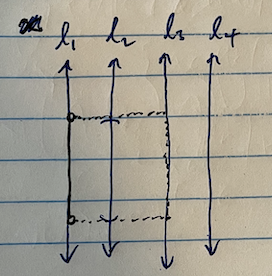
\includegraphics[scale=0.4]{img/1.png}
        \caption{$\ell_1, \ell_2$ intersect the open set at open intervals. $\ell_3, \ell_4$ does not but there are always open sets for which the intersection are open intervals. } 
        \label{fig:1}
      \end{figure}

      \item If $L$ is not vertical, then it is the lower limit topology (or upper limit topology depending on how you parameterize the line). 

      \begin{figure}[H]
        \centering 
        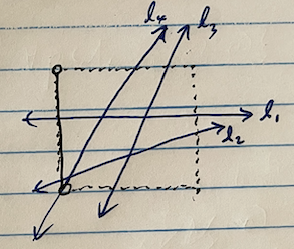
\includegraphics[scale=0.4]{img/2.png}
        \caption{All nonvertical lines will intersect the left ``closed'' side of some open set and will therefore induce the lower/upper limit topology on the line.}
        \label{fig:2}
      \end{figure}
    \end{enumerate}
    The basis of the product topology on $\mathbb{R}_\ell \times \mathbb{R}_\ell$ are all sets of form $[a, b) \times [c, d)$. 
    \begin{enumerate} 
      \item if $L$ has a negative slope (as in the graph represented by $y = mx + b$ where $m < 0$), then it is discrete topology since we can imagine the line intersecting the square at the lower-left corner.\footnote{We can also see it as the topology generated by the basis of closed intervals, but since $[a, b] \cap [b, c] = \{b\}$, this is equivalent to the discrete topology.} 

      \begin{figure}[H]
        \centering 
        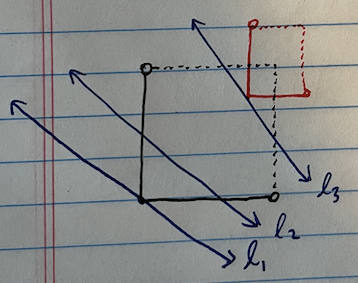
\includegraphics[scale=0.4]{img/3.png}
        \caption{We can construct an open set $[a, b) \times [c, d)$ where the point $(a, c)$ lies on any point on a negatively sloping line. This means that points are open sets, which generates the discrete topology. } 
        \label{fig:3}
      \end{figure}

      \item if $L$ vertical, horizontal, or has a positive slope, then it is the lower limit topology (or upper limit topology depending on how you parameterize the line). 

      \begin{figure}[H]
        \centering 
        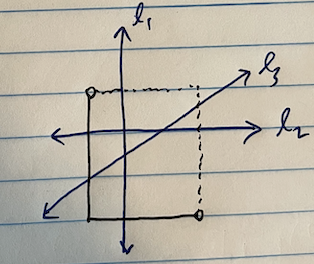
\includegraphics[scale=0.4]{img/4.png}
        \caption{If there is not a negative slope (vertical, horizontal, or positive sloping), then there is no way for a rectangle to intersect the line exactly at the lower-left corner without ``going through'' the rectangle. Therefore these examples generate half-open half-closed intervals on $L$. } 
        \label{fig:4}
      \end{figure}
    \end{enumerate}
  \end{solution}

  \begin{exercise}[Munkres 16.9]
    Show that the dictionary order topology on the set $\mathbb{R} \times \mathbb{R}$ is the same as the product topology $\mathbb{R}_d \times \mathbb{R}$, where $\mathbb{R}_d$ denotes $\mathbb{R}$ in the discrete topology. Compare this topology with the standard topology on $\mathbb{R}^2$.
  \end{exercise}

  \begin{exercise}[Munkres 16.10]
    Let $I = [0, 1]$. Compare the product topology on $I \times I$, the dictionary order topology on $I \times I$, and the topology $I \times I$ inherits as a subspace of $\mathbb{R} \times \mathbb{R}$ in the dictionary order topology.
  \end{exercise}

  \begin{exercise}[Math 411 Spring 2025, PS3]
    Let $P_n$ denote the set of polynomials in n variables with real coefficients. Any such polynomial defines a function on $\mathbb{R}^n$. If A is any subset of $P_n$, let $V(A) = \{x \in \mathbb{R}^n \mid p(x) = 0 \text{ for all } p \in A\}$. A subset $S \subset \mathbb{R}^n$ is called algebraic if it is equal to V(A) for some $A \subset P_n$.

    \begin{enumerate}
      \item Show that $\emptyset$ and $\mathbb{R}^n$ are both algebraic.

      \item Show that if $A_\alpha$ are subsets of $P_n$ (indexed by $\alpha \in I$ for some set I), then
      \[V\left(\bigcup_{\alpha\in I} A_\alpha\right) = \bigcap_{\alpha\in I} V(A_\alpha).\]
      In other words, any intersection of algebraic sets is algebraic.

      \item Suppose $A_1,\ldots,A_k$ are subsets of $P_n$. Let B be the set of polynomials that can be factored as $f = f_1 \cdots f_k$, where $f_i \in A_i$. Prove that
      \[V(B) = V(A_1) \cup \cdots \cup V(A_k).\]
      In other words, any finite union of algebraic sets is algebraic. (Hint: For the inclusion $V(B) \subset V(A_1) \cup \cdots \cup V(A_k)$, it may be easier to show that if $x \not\in V(A_1) \cup \cdots \cup V(A_k)$, then $x \not\in V(B)$.)

      \item Show that $\mathcal{T} = \{U \subset \mathbb{R}^n \mid \mathbb{R}^n - U \text{ is algebraic}\}$ is a topology on $\mathbb{R}^n$. This is known as the Zariski topology, named for the mathematician Oscar Zariski (1899-1986). It is very important in algebraic geometry and related fields.

      \item Show that for n = 1, the Zariski topology on $\mathbb{R}^1$ is precisely the finite complement topology.
    \end{enumerate}

    Note: Instead of doing this with $\mathbb{R}$, you could also do it with $\mathbb{C}$, $\mathbb{Q}$, or any other field.
  \end{exercise}
  \begin{solution}[a]
    Listed. 
    \begin{enumerate}
      \item Consider $A = \{ f(x) = 1\}$. Then $V(A) = \emptyset$ since $f$ never vanishes. 
      \item Consider $A = \{ f(x) = 0 \}$.Then $V(A) = \mathbb{R}^n$ since $f$ always vanishes. 
    \end{enumerate}
  \end{solution}
  \begin{solution}[b]
    We see that 
    \begin{align}
      V \bigg( \bigcup_{\alpha \in I} A_\alpha \bigg) & = \big\{ x \in \mathbb{R}^n \mid \forall p \in \cup_{\alpha \in I} A_\alpha ( p(x) = 0 )\big\} \\ 
                                                      & = \big\{ x \in \mathbb{R}^n \mid \forall \alpha \in I \forall p \in A_\alpha (p(x) = 0)  \big\} \\
                                                      & = \bigcap_{\alpha \in I} \big\{ x \in \mathbb{R}^n \mid \forall p \in A_\alpha (p(x) = 0) \big\} \\
                                                      & = \bigcap_{\alpha \in I} V(A_\alpha)
    \end{align}
  \end{solution}
  \begin{solution}[c]
    We prove bidirectionally. 
    \begin{enumerate}
      \item $\cup_{i} V(A_i) \subset V(B)$. Let $x \in \cup_i V(A_i)$. Then $x \in V(A_j)$ for some $1 \leq j \leq k$, which implies that $f_j (x) = 0$ for all $f_j \in A_j$. Therefore by the field properties of $\mathbb{R}$, 
      \begin{equation}
        f(x) = f_1 (x) \ldots \underbrace{f_j(x)}_{=0} \ldots f_k (x) = 0 
      \end{equation} 
      and therefore $f(x) = 0$ for all $f \in B$, which means that $x \in V(B)$. 

      \item $\cup_i V(A_i) \supset V(B)$. Assume that $x \not\in \cup_i V(A_i)$. Then for all $1 \leq i \leq k$, $x \not\in V(A_i)$, which implies that for all $i$ there exists some $f_i^{\ast} \in A_i$ s.t. $f_i^\ast (x) \neq 0$. Now construct the function $f^\ast = \prod_i f_i^\ast$, where $f_i^\ast \in A_i$, $f^\ast \in B$. But 
      \begin{equation}
        f^\ast (x) = \prod_{i=1}^k f_i^\ast (x) \neq 0
      \end{equation}
      since $f_i^\ast (x) \neq 0$ for all $i$, and so we have shown the existence of a function $f^\ast \in B$ such that $f^\ast (x) \neq 0$. Therefore $x \not\in V(B)$. 
    \end{enumerate}
  \end{solution}
  \begin{solution}[d] 
    We prove the properties of a topology. 
    \begin{enumerate}
      \item From (a), $\emptyset$ is algebraic $\implies \mathbb{R}^n \setminus \emptyset = \mathbb{R}^n$ is in $\mathscr{T}$. Also, $\mathbb{R}^n$ is algebraic $\implies \mathbb{R}^n \setminus \mathbb{R}^n = \emptyset$ is in $\mathscr{T}$.  

      \item Let $\{U_\alpha\}_{\alpha \in I}$ be a collection of open sets in $\mathscr{T}$. Then by definition $\mathbb{R}^n \setminus U_\alpha$ is algebraic, and 
      \begin{equation}
        \mathbb{R}^n \setminus \bigg( \bigcup_{\alpha \in I} U_\alpha \bigg) = \bigcap_{\alpha \in I} (\mathbb{R}^n \setminus U_\alpha) 
      \end{equation} 
      we know from (b) that arbitrary intersections of algebraic sets is algebraic, so the LHS is also algebraic, which by definition means the union is in $\mathscr{T}$. 

      \item Let $U_1, \ldots, U_k$ be a collection of open sets in $\mathscr{T}$. Then by definition $\mathbb{R}^n \setminus U_i$ is algebraic for $1 \leq i \leq k$, and  
      \begin{equation}
        \mathbb{R}^n \setminus \bigg( \bigcap_{i=1}^k U_i \bigg) = \bigcup_{i=1}^k (\mathbb{R}^n \setminus U_i)
      \end{equation}
      we know from (c) that finite unions of algebraic sets is algebraic, and so the LHS is also algebraic, which by definition means the finite intersection is in $\mathscr{T}$. 
    \end{enumerate}
  \end{solution}
  \begin{solution}[e]
    For an open set $U$, inclusion in the finite complement topology asserts that $\mathbb{R} \setminus U$ must be finite or $U = \emptyset$, and inclusion in the Zariski topology asserts that $\mathbb{R} \setminus U$ must be algebraic. Therefore it satisfies to show that the complements (within the universe of the power set) are equal, i.e. that the set of all finite subsets of $\mathbb{R}$ plus $\mathbb{R}$ itself and the set of all algebraic subsets of $\mathbb{R}$ is equal. Let us denote the former $S$ and the latter $T$. 
    \begin{enumerate}
      \item $S \subset T$. Let $Y \in S$ ($Y$ is a set). If $Y = \mathbb{R}$, then it is algebraic as shown in (a). Otherwise, it is finite and we can enumerate it as $Y = \{y_1, \ldots, y_n\}$, and define the singleton subset of polynomials 
      \begin{equation}
        A = \bigg\{ f(x) = \prod_{i=1}^n (x - y_i) \bigg\}
      \end{equation} 
      $V(A)$ consists of all reals where $f(x) = 0$, which happens exactly when $x = y_i$ for some $i$.\footnote{If not, then every $(x - y_i)$ is nonzero, and the product is nonzero.} Therefore, $Y = V(A) \implies Y$ is algebraic $\implies Y \subset T$. 

      \item $T \subset S$. Let $Y \in T$. Then we know that there exists some subset of polynomials $A$ such that $Y = V(A)$. If $A$ is empty, then $V(A) = \mathbb{R}$ since the predicate in the set-builder notation is vacuously true, and $\mathbb{R}$ is contained in the $S$. If $A$ is not empty, then there exists some polynomial $f$ from $A$. By definition it must be the case that for all $y \in Y$, $f(y) = 0$. We consider two cases. 
      \begin{enumerate}
        \item $f$ is constant. If $f \neq 0$, then $V(A) = \emptyset$, which is in $S$. If $f = 0$, then $V(A) = \mathbb{R}$, which is in $S$. 
        \item $f$ has degree $n \geq 1$. Since this is a polynomial ring over a field $\mathbb{F}[x]$, $f(y)$ cannot have more than $n$ real roots.\footnote{Using the single factor theorem of commutative rings we can use induction to prove that the set of roots cannot go beyond $n$. For linear polynomials $f(x) = mx + b$ there is one root $x = -b/m$ which satisfies the base case, and for higher degrees of $n$ we show that if there is a root where $p(a) = 0$, then $p(x) = (x - a) q(x)$ where $q$ is of degree $n-1$ which cannot have more than $n-1$ factors.} Therefore $|Y| \leq n$ and $Y$ must be finite. 
      \end{enumerate}

      We have shown that $V(\{f\})$ is finite. Since $V(A)$ consists of $y$'s that hold for all $f \in A$, $V(A) \subset V(\{f\})$.\footnote{To see why, look at my solution for (b).} The subset of finite sets is finite, and therefore $Y = V(A) \in S$. 
    \end{enumerate}
  \end{solution}

  \begin{exercise}[Munkres 19.4]
    Show that $(X_1 \times \cdots \times X_{n-1}) \times X_n$ is homeomorphic with $X_1 \times \cdots \times X_n$.
  \end{exercise}

  \begin{exercise}[Munkres 19.5]
    One of the implications stated in Theorem 19.6 holds for the box topology. Which one?
  \end{exercise}

  \begin{exercise}[Munkres 19.6]
    Let $\mathbf{x}_1, \mathbf{x}_2, \ldots$ be a sequence of the points of the product space $\prod X_\alpha$. Show that this sequence converges to the point $\mathbf{x}$ if and only if the sequence $\pi_\alpha(\mathbf{x}_1), \pi_\alpha(\mathbf{x}_2), \ldots$ converges to $\pi_\alpha(\mathbf{x})$ for each $\alpha$. Is this fact true if one uses the box topology instead of the product topology?
  \end{exercise}

  \begin{exercise}[Munkres 19.7]
    Let $\mathbb{R}^\infty$ be the subset of $\mathbb{R}^\omega$ consisting of all sequences that are ``eventually zero,'' that is, all sequences $(x_1, x_2, \ldots)$ such that $x_i \neq 0$ for only finitely many values of $i$. What is the closure of $\mathbb{R}^\infty$ in $\mathbb{R}^\omega$ in the box and product topologies? Justify your answer.
  \end{exercise}
  \begin{solution}
    In the box topology, $\overline{\mathbb{R}^\infty} = \mathbb{R}^\infty$. We show this by taking any sequence not in $\mathbb{R}^\infty$ and showing that there exists an open neighborhood that has a trivial intersection with $\mathbb{R}^\infty$. Consider a non-eventually zero sequence $y \in \mathbb{R}^\omega \setminus \mathbb{R}^\infty$, which must have an infinite number of nonzero terms. $y$ is contained within the open set (in the box topology) 
    \begin{equation}
      U = U_1 \times U_2 \times \ldots, \qquad U_i = 
      \begin{cases}
        (0, +\infty) & \text{ if } y_i > 0 \\
        (-1, 1)  & \text{ if } y_i = 0 \\
        (-\infty, 0) & \text{ if } y_i < 0
      \end{cases}
    \end{equation}
    This is an open set that clearly contains $y$, but it has an empty intersection with $\mathbb{R}^\omega$ since there are an infinite number of nonzero terms $y_i$ and so there are an infinite number of $U_i$'s that do not contain $0$. 

    In the product topology, basis elements are all sets of the form $\prod U_i$ where $U_i$ is open in $\mathbb{R}$ and $U_i = \mathbb{R}$ except for finitely many values of $i$. Therefore, $U_i \neq \mathbb{R}$ for finite values. Now given any sequence $y \in \mathbb{R}^\omega$, we claim that it is a limit point of $\mathbb{R}^\infty$. An open neighborhood of $y$ of form $U_y = \prod U_i$ must have some maximum index $N$ for which $U_i = \mathbb{R}$ when $i > N$, and so the eventually-zero sequence $x = (y_1, y_2, \ldots, y_N, 0, 0 ,\ldots)$ must be in $U$, implying that $U_y \cap \mathbb{R}^\infty \neq \emptyset$, and so $y$ is a limit point of $U_y$. Therefore all sequences are limit points, which means $\overline{\mathbb{R}^\infty} = \mathbb{R}^\omega$. 
  \end{solution}

  \begin{exercise}[Munkres 19.8]
    Given sequences $(a_1, a_2, \ldots)$ and $(b_1, b_2, \ldots)$ of real numbers with $a_i > 0$ for all $i$, define $h : \mathbb{R}^\omega \to \mathbb{R}^\omega$ by the equation
    \begin{equation}
      h((x_1, x_2, \ldots)) = (a_1x_1 + b_1, a_2x_2 + b_2, \ldots).
    \end{equation}
    Show that if $\mathbb{R}^\omega$ is given the product topology, $h$ is a homeomorphism of $\mathbb{R}^\omega$ with itself. What happens if $\mathbb{R}^\omega$ is given the box topology?
  \end{exercise}
  \begin{solution}
    We first show $h$ is a bijection. Indeed, the element-wise mappings are bijections and the inverse is 
    \begin{equation}
      h^{-1} ((x_1, \ldots, )) = \bigg(\ldots,  \frac{x_i - b_i}{a_i}, \ldots \bigg)
    \end{equation} 
    Now we show that it is continuous. Given an open set in $\mathbb{R}^\omega$ in the product topology, it has the form 
    \begin{equation}
      U = (l_1, u_1) \times (l_2, u_2) \times \ldots \times (l_n, u_n) \times \mathbb{R} \times \ldots 
    \end{equation} 
    The preimage under $h$ is 
    \begin{equation}
      h^{-1} (U) = \bigg( \frac{l_1 - b_1}{a_1}, \frac{u_1 - b_1}{a_1} \bigg) \times \ldots \times \bigg( \frac{l_n - b_n}{a_n}, \frac{u_n - b_n}{a_n} \bigg) \times \mathbb{R} \times \ldots
    \end{equation}
    where $l_1 < u_1 \implies (l_1 - b_1) /a_1 < (u_1 - b_1) / a_1$. This is also of the form of open sets in the product topology, and therefore is continuous. Now considering the continuity of the inverse function, we can see that taking the same $U$ as before, we have 
    \begin{equation}
      h(U) = (a_1 l_1 + b_1, a_1 u_1 + b_1) \times \ldots \times (a_n l_n + b_n, a_n u_n + b_n) \times \mathbb{R} \ldots 
    \end{equation}
    which is also open in the product topology. Therefore $h$ is a homeomorphism under the product topologies. 

    Now we consider the box topology. Given an box-topology open set of the form 
    \begin{equation}
      U = (l_1, u_1) \times (l_2, u_2) \times \ldots
    \end{equation} 
    then the preimage and image are 
    \begin{align}
      h^{-1} (U) & = \bigg( \frac{l_1 - b_1}{a_1}, \frac{u_1 - b_1}{a_1} \bigg) \times \bigg( \frac{l_2 - b_2}{a_2}, \frac{u_2 - b_2}{a_2} \bigg) \times \ldots \\
      h(U) & = h(U) = (a_1 l_1 + b_1, a_1 u_1 + b_1) \times (a_2 l_2 + b_2, a_2 u_2 + b_2) \times 
    \end{align}
    which are both open in the box topology and so $h$ and $h^{-1}$ are continuous. Thus $h$ is also a homeomorphism. 
  \end{solution}

  \begin{exercise}[Munkres 19.9]
    Show that the choice axiom is equivalent to the statement that for any indexed family $\{A_\alpha\}_{\alpha \in J}$ of nonempty sets, with $J \neq \emptyset$, the cartesian product
    \begin{align*}
      \prod_{\alpha \in J} A_\alpha
    \end{align*}
    is not empty.
  \end{exercise}

  \begin{exercise}[Munkres 19.10]
    Let $A$ be a set; let $\{X_\alpha\}_{\alpha \in J}$ be an indexed family of spaces; and let $\{f_\alpha\}_{\alpha \in J}$ be an indexed family of functions $f_\alpha : A \to X_\alpha$.
    \begin{enumerate}
      \item Show there is a unique coarsest topology $\mathcal{T}$ on $A$ relative to which each of the functions $f_\alpha$ is continuous.
      \item Let
      \begin{align*}
        S_\beta = \{f_\beta^{-1}(U_\beta) \mid U_\beta \text{ is open in } X_\beta\},
      \end{align*}
      and let $S = \bigcup S_\beta$. Show that $S$ is a subbasis for $\mathcal{T}$.
      \item Show that a map $g : Y \to A$ is continuous relative to $\mathcal{T}$ if and only if each map $f_\alpha \circ g$ is continuous.
      \item Let $f : A \to \prod X_\alpha$ be defined by the equation
      \begin{align*}
        f(a) = (f_\alpha(a))_{\alpha \in J};
      \end{align*}
      let $Z$ denote the subspace $f(A)$ of the product space $\prod X_\alpha$. Show that the image under $f$ of each element of $\mathcal{T}$ is an open set of $Z$.
    \end{enumerate}
  \end{exercise}

  \begin{exercise}[Munkres 22.2]
    \begin{enumerate}
      \item[(a)] Let $p : X \to Y$ be a continuous map. Show that if there is a continuous map
        $f : Y \to X$ such that $p \circ f$ equals the identity map of $Y$, then $p$ is a quotient
        map.
      
      \item[(b)] If $A \subset X$, a \textit{retraction} of $X$ onto $A$ is a continuous map $r : X \to A$ such
        that $r(a) = a$ for each $a \in A$. Show that a retraction is a quotient map.
    \end{enumerate}
  \end{exercise}
  \begin{solution}
     Listed. 
     \begin{enumerate}
       \item Let $U \subset Y$, and let $p^{-1}(U)$ be open. Then, 
       \begin{align}
         p^{-1} (U) \subset X \text{ open} & \implies f^{-1} (p^{-1}(U)) \subset Y \text{ open} \\
                                           & \implies (p \circ f)^{-1} (U) = U \subset Y \text{ open}
       \end{align}
       and since $p$ is continuous, $p$ is a quotient map. Since $p \circ f$ equals the identity map, it must be the case that $p$ is surjective. 

       \item We know that the canonical injection $\iota: A \rightarrow X$ is continuous, and $r \circ \iota = I$, the identity map of $A$. Therefore by (a), $p$ is a quotient map. 
     \end{enumerate}
  \end{solution}

  \begin{exercise}[Munkres 22.3]
    Let $\pi_1 : \mathbb{R} \times \mathbb{R} \to \mathbb{R}$ be projection on the first coordinate. Let $A$ be the subspace of $\mathbb{R} \times \mathbb{R}$ consisting of all points $x \times y$ for which either $x \geq 0$ or $y = 0$ (or both); let $q : A \to \mathbb{R}$ be obtained by restricting $\pi_1$. Show that $q$ is a quotient map that is neither open nor closed.
  \end{exercise}
  \begin{solution} 
    The restriction of a continuous function is always continuous, so $q$ is continuous. Furthermore $q$ is surjective since given any $x \in \mathbb{R}$, we can always see that $(x, 0) \in q^{-1}(\{x\})$. Finally, let $U \subset \mathbb{R}$ s.t. $q^{-1} (U) \subset A$ is open. Then, for any $x \in U$, we know $(x, 0) \subset q^{-1} (U)$, and so  $\exists \epsilon > 0$ s.t. $B((x, 0), \epsilon) \cap A) \subset q^{-1} (U)$. Mapping both sides through $q$ again gives 
    \begin{equation}
      (x - \epsilon, x + \epsilon) = q\big( B((x, 0), \epsilon) \cap A) \big) \subset q (q^{-1}(U)) = U
    \end{equation}
    and so $U$ is open. Therefore, $q$ is a quotient map. To see why it is not open, consider the open set of $A$ 
    \begin{equation}
      U = [0, 1) \times (0, 1) = [(-1, 1) \times (0, 1)] \cap A 
    \end{equation} 
    Then $q(U) = [0, 1)$ which is not open in $\mathbb{R}$. To see why not closed, consider the closed set $C = \{(x, y) \in \mathbb{R}^2 \mid xy = 1, x > 0 \}$.\footnote{Also stated to be closed by example 2 of chapter 22.} Then $p(C) = (0, +\infty)$ which is not closed in $\mathbb{R}$. 
  \end{solution}

  \begin{exercise}[Munkres 22.4]
    \begin{enumerate}
      \item[(a)] Define an equivalence relation on the plane $X = \mathbb{R}^2$ as follows:
      \begin{center}
        $x_0 \times y_0 \sim x_1 \times y_1$ \quad if $x_0 + y_0^2 = x_1 + y_1^2$.
      \end{center}
      Let $X^*$ be the corresponding quotient space. It is homeomorphic to a familiar
      space; what is it? 
      
      \item[(b)] Repeat (a) for the equivalence relation
      \begin{center}
        $x_0 \times y_0 \sim x_1 \times y_1$ \quad if $x_0^2 + y_0^2 = x_1^2 + y_1^2$.
      \end{center}
    \end{enumerate}
  \end{exercise}
  \begin{solution}
    Listed. 
    \begin{enumerate}
      \item Graphing this shows that $X^\ast$ is the set of all horizontal parabolas of the same scale and opening leftwards with the vertex on the $x$-axis, i.e. the elements are just left-right shifts of one another. We claim that it is homeomorphic to $\mathbb{R}$. Let $p: \mathbb{R}^2 \rightarrow X^\ast$ be the quotient map and $f: \mathbb{R}^2 \rightarrow \mathbb{R}$ be defined $f(x, y) = x + y^2$, which satisfies $(x,y) \sim (x^\prime, y^\prime) \iff f(x, y) = f(x^\prime, y^\prime)$. Therefore, this induces a function $\bar{f}: X^\ast  \rightarrow \mathbb{R}$ s.t. $\bar{f} \circ p = f$. Since $f$ is continuous, $\bar{f}$ is continuous. Also, we can see that $\bar{f}$ is a bijection since we can map every element in the equivalence class of $[(x, y)]$ s.t. $x + y^2 = c$ to $c \in \mathbb{R}$. Finally, we show that $\bar{f}^{-1}$ is continuous. We can think of $\bar{f}^{-1}$ as the composition of maps $c \mapsto (c, 0) \mapsto [(c, 0)]$, where the first map is trivially continuous and the second map is $p$, which is also continuous. Therefore $\bar{f}^{-1}$ is continuous, and it is a homeomorphism. 
        
      \item We can see that $X^\ast$ is the set of all circles of nonnegative radius (the origin is a circle of radius $0$), and we claim that it is homeomorphic to $[0, +\infty)$. Let $p: \mathbb{R}^2 \rightarrow X^\ast$ be the quotient map and $f: \mathbb{R}^2 \rightarrow [0, +\infty)$ be defined $f(x, y) = x^2 + y^2$, which satisfies $(x,y) \sim (x^\prime, y^\prime) \iff f(x, y) = f(x^\prime, y^\prime)$. Therefore, this induces a function $\bar{f}: X^\ast  \rightarrow [0, +\infty)$ s.t. $\bar{f} \circ p = f$. Since $f$ is continuous, $\bar{f}$ is continuous. Also, we can see that $\bar{f}$ is a bijection since we can map every element in the equivalence class of $[(x, y)]$ s.t. $x^2 + y^2 = c$ to $c \in [0, +\infty)$. Finally, we show that $\bar{f}^{-1}$ is continuous. We can think of $\bar{f}^{-1}$ as the composition of maps $c \mapsto (\sqrt{c}, 0) \mapsto [(\sqrt{c}, 0)]$, where the first map is continuous\footnote{The square root function from $\mathbb{R}_0^+$ to itself is continuous since the preimage of an open interval $(a, b)$ is $(\sqrt{a}, \sqrt{b})$ which is also open in $\mathbb{R}_0^+$, and for $[0, b)$ the preimage is $[0, \sqrt{b})$.} and the second map is $p$, which is also continuous. Therefore $\bar{f}^{-1}$ is continuous, and it is a homeomorphism. 
    \end{enumerate}
  \end{solution}

  \begin{exercise}[Munkres 22.5]
    Let $p : X \to Y$ be an open map. Show that if $A$ is open in $X$, then the map $q : A \to p(A)$ obtained by restricting $p$ is an open map.
  \end{exercise}

  \begin{exercise}[Munkres 22.6]
    Recall that $\mathbb{R}_K$ denotes the real line in the $K$-topology. (See \S13.) Let $Y$ be the quotient space obtained from $\mathbb{R}_K$ by collapsing the set $K$ to a point; let $p : \mathbb{R}_K \to Y$ be the quotient map.
    \begin{enumerate} 
      \item[(a)] Show that $Y$ satisfies the $T_1$ axiom, but is not Hausdorff.
      \item[(b)] Show that $p \times p : \mathbb{R}_K \times \mathbb{R}_K \to Y \times Y$ is not a quotient map. [Hint: The diagonal is not closed in $Y \times Y$, but its inverse image is closed in $\mathbb{R}_K \times \mathbb{R}_K$.]
    \end{enumerate}
  \end{exercise}

  \begin{exercise}[Math 411 Spring 2025, PS6]
    For each integer $n \geq 1$, let us consider the following spaces:
    \begin{align*}
      S^n &= \{\mathbf{x} \in \mathbb{R}^{n+1} \mid \|\mathbf{x}\|= 1\} \\
      X^{n+1} &= \mathbb{R}^{n+1} - \{\mathbf{0}\}
    \end{align*}
    (Note: the superscript is just a decoration that indicates the ``dimensionality''
    of the space; it does \textit{not} indicate raising something to a power.)
    \begin{enumerate}
      \item[(1)] Show that the function $r : X^{n+1} \to S^n$ defined by $r(\mathbf{x}) = \mathbf{x}/\|\mathbf{x}\|$ is a
        quotient map, and describe the corresponding equivalence relation. (Hint:
        Use \#2 from \S22.)
        
      \item[(2)] We now define a space called \textit{real projective n-space}, or $\mathbb{RP}^n$. We can
        define it in either of two ways:
        \begin{enumerate}
          \item[(a)] $X^{n+1}/{\sim}$, where $\mathbf{x} \sim \mathbf{y}$ iff $\mathbf{x} = \lambda\mathbf{y}$ for some $\lambda \in \mathbb{R} - \{0\}$.
          \item[(b)] $S^n/{\sim}$, where $\mathbf{x} \sim \mathbf{y}$ iff $\mathbf{x} = \pm\mathbf{y}$.
        \end{enumerate}
        Let $p : X^{n+1} \to \mathbb{RP}^n$ be the quotient map. Prove that $p|_{S^n} : S^n \to \mathbb{RP}^n$ is
        also a quotient map, and hence that the two descriptions above produce
        homeomorphic spaces. (Hint: It may help to observe that $p|_{S^n} \circ r = p$.)
        
      \item[(3)] Using the description of $\mathbb{RP}^n$ as a quotient of $S^n$, prove that $\mathbb{RP}^n$ is
        a Hausdorff space. (Hint: note that for $\mathbf{x} \in S^n$ and $\epsilon > 0$, the set
        $(B(\mathbf{x},\epsilon) \cup B(-\mathbf{x},\epsilon)) \cap S^n$ is open and saturated.)
        
      \item[(4)] Let $D^n_+$ denote the ``upper hemisphere'' in $S^n$: $D^n_+ = \{\mathbf{x} \in S^n \mid x_{n+1} \geq 0\}$.
        Show that $D^n_+$ is homeomorphic to $D^n = \{\mathbf{x} \in \mathbb{R}^n \mid \|\mathbf{x}\| \leq 1\}$, the unit
        disk in $\mathbb{R}^n$.
        
      \item[(5)] The restriction of $p$ to $D^n$, viewed as a map $D^n \to \mathbb{RP}^n$, can be shown
        to be a quotient map. Assuming this, describe an equivalence relation
        on $D^n$ whose quotient space is homeomorphic to $\mathbb{RP}^n$. In the case where
        $n = 2$, describe how we may concretely describe $\mathbb{RP}^2$ as a ``video game.''
    \end{enumerate}
  \end{exercise}
  \begin{solution}
    Listed. 
    \begin{enumerate}
      \item We claim $r$ is a retraction, since $r(x) = x$ for all $x \in S^n \subset \mathbb{R}^{n+1}$. $r$ is also continuous since a basis element of the topology of $S^n$ can be written $B = \big\{(a_1, b_1) \times \ldots \times (a_{n+1}, b_{n+1}) \big\} \cap S^n$. Therefore the preimage of such a set is 
      \begin{equation}
        r^{-1} (B) = \bigcup_{c > 0} \big\{(c a_1, c b_1) \times \ldots \times (c a_{n+1}, c b_{n+1}) \big\} \cap S^n 
      \end{equation}
      which is the union of open sets in $S^n$ and therefore is open in $S^n$. From the first exercise, $r$ is a quotient map. It consists of each ray starting from the origin, and maps each direction to the unit vector, creating a sphere.   


      \item $p|_{S^n} \circ r = p$. Since $p$ is a quotient map, it is continuous and its restriction $p|_{S^n}$ is also continuous. Since $p$ is a quotient map, it is surjective and therefore $p|_{S^n}$ must be surjective.\footnote{If $p|_{S^n}$ wasn't surjective, then $p|_{S^n} \circ r$ is not surjective and $p$ is not surjective, a contradiction. } Now let $U \subset \mathbb{RP}^n$ s.t. $p|_{S^n}^{-1} (U)$ is open in $S^n$. Then, 
      \begin{equation}
        r^{-1} \big( p|_{S^n}^{-1} (U) \big) = (p |_{S^n} \circ r)^{-1} (U) = p^{-1} (U)
      \end{equation} 
      is open since $r$ is continuous. But since $p$ is a quotient map, $U$ is open, implying that $p|_{S^n}$ is a quotient map. Therefore, we have shown that 
      \begin{equation}
        X^{n+1} / \sim \cong \mathbb{RP}^n \text{ and } S^n / \sim \cong \mathbb{RP}^n \implies X^{n+1} / \sim \cong S^n / \sim
      \end{equation}

      \item Let us have $x, y \in \mathbb{RP}^n$ with $x \neq y$. Then there exists $u, v \in S^n$ s.t. $p|_{S^n}^{-1}(x) = \{u, -u\}$ and $p|_{S^n}^{-1} (y) = \{v, -v\}$. We can let $\epsilon = \frac{1}{2} \min\{ \|u - v\|, \|u + v\|\}$, which means that 
      \begin{equation}
        B(\pm u, \epsilon) \cap B(\pm v, \epsilon) = \emptyset 
      \end{equation}
      in $\mathbb{R}^n$, and so the open neighborhoods around $\pm u, \pm v$, denoted $U_{\pm}, V_{\pm}$ are all pairwise disjoint in $S^n$. Note that $U_+ \cup U_-$ and $V_+ \cup V_-$ are open, saturated, and disjoint, and so $p|_{S^n}$, as a quotient map, maps both of these sets to disjoint open neighborhoods of $x, y$, proving that $\mathbb{RP}^n$ is Hausdorff. 

      \item We can visualize this as if we were just ``pushing up'' the disk onto the hemisphere. More formally, let us define $f: D^n \rightarrow D_+^n$ as 
      \begin{equation}
        f(x) = f(x_1, \ldots, x_n) = (x_1, \ldots, x_n, \sqrt{1 - \|x\|})
      \end{equation}
      This is well-defined since we assume that $\|x\| \leq 1$. This is trivially injective since changing any of the $x_i$'s will result in a different values in the first $n$ terms of the output. It is surjective since given any element $y = (y_1, \ldots, y_{n+1}) \in D_+$, we know that $\|y\| = 1$ and so we can find the preimage to be $x = (y_1, \ldots, y_n)$ which will satisfy $\|x\| \leq 1$. Therefore, $f$ is bijective, with the inverse function 
      \begin{equation}
        f^{-1} (y) = f^{-1} (y_1, \ldots, y_{n+1}) = (y_1, \ldots, y_{n})
      \end{equation}
      To prove continuity of $f$, consider the basis element of the form 
      \begin{equation}
        (a_1, b_1) \times \ldots \times (a_{n+1}, b_{n+1}) \cap D_+^n 
      \end{equation}
      the preimage is 
      \begin{equation}
        f^{-1} \big( (a_1, b_1) \times \ldots \times (a_{n+1}, b_{n+1})\big) \cap f^{-1} (D_+^n) = (a_1, b_1) \times (a_n, b_n) \cap D^n 
      \end{equation}
      which is a basis element of $D^n$. To prove continuity of $f^{-1}$, we consider its extension $f^{-1}: \mathbb{R}^{n+1} \rightarrow \mathbb{R}^n$, which is simply a projection of the first $n$ elements and is therefore continuous. The restriction of this function $f^{-1}: D_+^n \rightarrow \mathbb{R}^n$ is therefore continuous, and since the image of $f^{-1}$ only hits $D^n$, every open set in $D^n$ is of the form $U = V \cap D^n$ for $V$ open in $\mathbb{R}^n$, where the preimage will simply be $f(U) = f(V) \cap f(D^n)$. We know $f(V)$ is open\footnote{by continuity of $f^{-1}$ with codomain $\mathbb{R}^n$} and $f(D^n) = D^n_+$, $f(U)$ is open in $D_+^n$. 

      \item In $D^n$, we define the equivalence relation $\sim$ where $x \sim -x$ if $\|x\| = 1$, and every other point (in the interior of the disk) is equivalent to itself only. When $n=2$, we can imagine a player walking in a circular disk in $\mathbb{R}^2$, and when it crosses the boundary it will end up at the antipodal point. 
    \end{enumerate}
  \end{solution}
